%%%%%%%%%%%%%%%%%%%%%%%%%%%%%%%%%%%%%%%%%
% Masters/Doctoral Thesis 
% LaTeX Template
% Version 1.42 (19/1/14)
%
% This template has been downloaded from:
% http://www.latextemplates.com
%
% Original authors:
% Steven Gunn 
% http://users.ecs.soton.ac.uk/srg/softwaretools/document/templates/
% and
% Sunil Patel
% http://www.sunilpatel.co.uk/thesis-template/
%
% License:
% CC BY-NC-SA 3.0 (http://creativecommons.org/licenses/by-nc-sa/3.0/)
%
% Note:
% Make sure to edit document variables in the Thesis.cls file
%
%%%%%%%%%%%%%%%%%%%%%%%%%%%%%%%%%%%%%%%%%

%----------------------------------------------------------------------------------------
%	PACKAGES AND OTHER DOCUMENT CONFIGURATIONS
%----------------------------------------------------------------------------------------
% Paper size, default font size and one-sided paper
\documentclass[11pt, a4paper, oneside]{Thesis} 

% Specifies the directory where pictures are stored
\graphicspath{{Pictures/}} 

% Use the natbib reference package - read up on this to edit the reference style
\usepackage[square, numbers, comma, sort&compress]{natbib} 

\usepackage{microtype}
\DisableLigatures{encoding=*,family=*}

\usepackage{hyperref}

\usepackage{color}
% Colors hyperlinks in blue - change to black if annoying
\hypersetup{urlcolor=black, 
	linkcolor=black, 
	citecolor=black,
	colorlinks=true} 


\usepackage{colortbl}
\definecolor{LightCyan}{rgb}{0.88,1,1}

\usepackage{listings}
\usepackage{setspace}
\usepackage{siunitx}


\definecolor{Code}{rgb}{0,0,0}
\definecolor{Decorators}{rgb}{0.5,0.5,0.5}
\definecolor{Numbers}{rgb}{0.5,0,0}
\definecolor{MatchingBrackets}{rgb}{0.25,0.5,0.5}
\definecolor{Keywords}{rgb}{0,0,1}
\definecolor{self}{rgb}{0,0,0}
\definecolor{Strings}{rgb}{0,0.63,0}
\definecolor{Comments}{rgb}{0,0.63,1}
\definecolor{Backquotes}{rgb}{0,0,0}
\definecolor{Classname}{rgb}{0,0,0}
\definecolor{FunctionName}{rgb}{0,0,0}
\definecolor{Operators}{rgb}{0,0,0}
\definecolor{Background}{rgb}{0.98,0.98,0.98}

\lstset{
numbers=left,
numberstyle=\footnotesize,
numbersep=1em,
xleftmargin=1em,
framextopmargin=2em,
framexbottommargin=2em,
showspaces=false,
showtabs=false,
showstringspaces=false,
frame=l,
tabsize=4,
% Basic
basicstyle=\ttfamily\small\setstretch{1.0},
backgroundcolor=\color{Background},
language=Python,
% Comments
commentstyle=\color{Comments}\slshape,
% Strings
stringstyle=\color{Strings},
morecomment=[s][\color{Strings}]{"""}{"""},
morecomment=[s][\color{Strings}]{'''}{'''},
% keywords
morekeywords={import,from,class,def,for,while,if,is,in,elif,else,not,and,or,print,break,continue,return,True,False,None,access,as,,del,except,exec,finally,global,import,lambda,pass,print,raise,try,assert,split,find,strip,get_text},
keywordstyle={\color{Keywords}\bfseries},
% additional keywords
morekeywords={[2]@invariant},
keywordstyle={[2]\color{Decorators}\slshape},
emph={self},
emphstyle={\color{self}\slshape},
captionpos=top
%
}

\usepackage{caption}
\DeclareCaptionFont{white}{\color{white}}
\DeclareCaptionFormat{listing}{\colorbox[cmyk]{0.43, 0.35, 0.35,0.01}{\parbox{\textwidth}{\hspace{15pt}#1#2#3}}}
\captionsetup[lstlisting]{format=listing,labelfont=white,textfont=white, singlelinecheck=false, margin=0pt, font={bf,footnotesize}}


\usepackage{booktabs}

\usepackage{spverbatim}

% Defines the thesis title - don't touch this
\title{\ttitle} 

\begin{document}

% Use roman page numbering style (i, ii, iii, iv...) for the pre-content pages
\frontmatter 

\setstretch{1.5} % Line spacing of 1.5

% Define the page headers using the FancyHdr package and set up for one-sided printing
% Clears all page headers and footers
\fancyhead{} 
% Sets the right side header to show the page number
\rhead{\thepage} 
% Clears the left side page header
\lhead{} 

% Finally, use the "fancy" page style to implement the FancyHdr headers
\pagestyle{fancy} 

% New command to make the lines in the title page
\newcommand{\HRule}{\rule{\linewidth}{0.5mm}} 

% PDF meta-data
\hypersetup{pdftitle={\ttitle}}
\hypersetup{pdfsubject=\subjectname}
\hypersetup{pdfauthor=\authornames}
\hypersetup{pdfkeywords=\keywordnames}

%----------------------------------------------------------------------------------------
%	TITLE PAGE
%----------------------------------------------------------------------------------------

\begin{titlepage}
\begin{center}

% University name
\textsc{\LARGE \univname}\\[1.5cm] 
% Thesis type
\textsc{\Large Masters Thesis}\\[0.5cm] 

% Horizontal line
\HRule \\[0.4cm] 

% Thesis title
{\huge \bfseries \ttitle}\\[0.4cm] 

% Horizontal line
\HRule \\[1.5cm] 
 
\begin{minipage}{0.4\textwidth}
\begin{flushleft} \large
\emph{Author:}\\
% Author name - remove the \href bracket to remove the link
{\authornames} 
\end{flushleft}
\end{minipage}
\begin{minipage}{0.4\textwidth}
\begin{flushright} \large
\emph{Supervisor:} \\
% Supervisor name - remove the \href bracket to remove the link
{\supname}   
\end{flushright}
\end{minipage}\\[3cm]
 
% University requirement text
\large \textit{A thesis submitted in partial fulfilment of the requirements\\ for the degree of \degreename}\\[0.3cm] 
\textit{at}\\[0.4cm]

% Research group name and department name
\univname\\\addressnames\\[2cm] 
 
% Date
{\large \today}\\[4cm] 

% University/department logo - uncomment to place it
%\includegraphics{Logo} 
 
\vfill
\end{center}
\end{titlepage}


%----------------------------------------------------------------------------------------
%	DECLARATION PAGE
%	Your institution may give you a different text to place here
%----------------------------------------------------------------------------------------

\Declaration{

% Add a gap in the Contents, for aesthetics
\addtocontents{toc}{\vspace{1em}} 

I hereby certify that this material, which I now submit for assessment on the programme of study leading to the award of \textbf{M.Sc. in Computing} in the Institute of Technology Blanchardstown, is entirely my own work except where otherwise stated, and has not been submitted for assessment for an academic purpose at this or any other academic institution other than in partial fulfilment of the requirements of that stated above. \\

Signed [David Colton]: \\

% This prints a line for the signature
\rule[1em]{30em}{0.5pt} 


Date:\\

% This prints a line to write the date
\rule[1em]{30em}{0.5pt} 
}

%\clearpage % Start a new page

%----------------------------------------------------------------------------------------
%	QUOTATION PAGE
%----------------------------------------------------------------------------------------

%\pagestyle{empty} % No headers or footers for the following pages

%\null\vfill % Add some space to move the quote down the page a bit

%\textit{``Need a good quote to go here ...!"}

%\begin{flushright}
%Dave Barry
%\end{flushright}

%\vfill\vfill\vfill\vfill\vfill\vfill\null % Add some space at the bottom to position the quote just right

\clearpage % Start a new page

%----------------------------------------------------------------------------------------
%	ABSTRACT PAGE
%----------------------------------------------------------------------------------------

% Add the "Abstract" page entry to the Contents
\addtotoc{Abstract} 

% Add a gap in the Contents, for aesthetics
\abstract{\addtocontents{toc}{\vspace{1em}} 
The internet technology boom has led to a proliferation of tablets, laptops and smart phones with high-speed internet access. This access, coupled with the advent of instant messaging, chat rooms and social media websites, has led to an internet generation who think nothing of posting selfies, mood updates, their relationship status or anything about their life on-line. The traditional bully was the kid in school, or office worker, who got pleasure from watching their victims suffer as they verbally abused them or perhaps made fun of them or maybe even threatened them with violence. At least the victim knew who the bully was and, although not a solution, could plan their day to avoid crossing paths with the bully and having to suffer further torment. However, the bully has also moved on-line. This cyberbully now has twenty-four hour access to a potentially unlimited number of victims. Through their mean and harassing posts and comments the consequences of their cyberbullying activity is too often read about in the papers following another tragic teen suicide. To prevent this new form of bullying, it is important that technology is used to detect these cyberbullying posts.

This dissertation shows that Python, together with the application of text mining techniques, can be successfully used in the automatic detection of cyberbullying text. The contributions of this paper are many. To begin, a comprehensive literature review of the current trends in cyberbullying detection is provided. A new classified cyberbullying dataset, including detailed descriptions of the criteria used in its classification, is generated. An in-depth analysis of several classifiers, including multiple approaches to tackle class imbalance, is undertaken before a novel way of determining the best overall classifier using the recall values of both the positive and negative class in addition to considering the execution time of the model and penalising any data manipulation performed when tackling class imbalance is suggested. Finally, an evaluation of the best models is performed by simulating their evolution as new, previously unseen, samples are classified and then included as training data for subsequent iterations.}

\clearpage % Start a new page

%----------------------------------------------------------------------------------------
%	ACKNOWLEDGEMENTS
%----------------------------------------------------------------------------------------

% Reset the line-spacing to 1.3 for body text (if it has changed)
\setstretch{1.3} 

% Add a gap in the Contents, for aesthetics
\acknowledgements{\addtocontents{toc}{\vspace{1em}} 

\begin{quote}
 “The only people with whom you should try to get even are those who have helped you.”

 \em John E. Southard

\end{quote}

Niamh, Emma, Saoirse and Eva. Without your help, patience and the time you gave me, this masters would not have been possible. Time to get even.

\begin{quote}
"Some people talk in their sleep. \\
Lecturers talk while other people sleep."

 \em Albert Camus
\end{quote}

I'm very happy to say that this was not something that afflicted me over the last two years while completing this masters degree programme. First, a special thank you to Dr. Markus Hofmann who acted as my supervisor on this dissertation. This paper would not be what it is today without his thoughts and guidance from when the first green shoot of this work started showing, right up to the end. I must thank Geraldine Grey, Laura Keyes and Markus for their enthusiasm and passion for the subjects covered. 

}
\clearpage % Start a new page

%----------------------------------------------------------------------------------------
%	LIST OF CONTENTS/FIGURES/TABLES PAGES
%----------------------------------------------------------------------------------------

\pagestyle{fancy} % The page style headers have been "empty" all this time, now use the "fancy" headers as defined before to bring them back

\lhead{\emph{Contents}} % Set the left side page header to "Contents"
\tableofcontents % Write out the Table of Contents

\lhead{\emph{List of Figures}} % Set the left side page header to "List of Figures"
\listoffigures % Write out the List of Figures

\lhead{\emph{List of Tables}} % Set the left side page header to "List of Tables"
\listoftables % Write out the List of Tables

%----------------------------------------------------------------------------------------
%	DEDICATION
%----------------------------------------------------------------------------------------

\setstretch{1.3} % Return the line spacing back to 1.3

\pagestyle{empty} % Page style needs to be empty for this page

\dedicatory{For Niamh, Emma, Saoirse and Eva} % Dedication text

\addtocontents{toc}{\vspace{2em}} % Add a gap in the Contents, for aesthetics

%----------------------------------------------------------------------------------------
%	THESIS CONTENT - CHAPTERS
%----------------------------------------------------------------------------------------

\mainmatter % Begin numeric (1,2,3...) page numbering

\pagestyle{fancy} % Return the page headers back to the "fancy" style

% Include the chapters of the thesis as separate files from the Chapters folder
% Uncomment the lines as you write the chapters

% Chapter Template

\chapter{Introduction} % Main chapter title

\label{chapter1} % Change X to a consecutive number; for referencing this chapter elsewhere, use \ref{ChapterX}

\lhead{Chapter 1. \emph{Introduction}} % Change X to a consecutive number; this is for the header on each page - perhaps a shortened title

\begin{quotation}
``Bullying is any unwanted aggressive behaviour(s) by another youth or group of youths who are not siblings or current dating partners that involves an observed or perceived power imbalance and is repeated multiple times or is highly likely to be repeated. Bullying may inflict harm or distress on the targeted youth including physical, psychological, social, or educational harm.'' \\ 
\citet{assistant_secretary_for_public_affairs_what_2014}.
\end{quotation}

\begin{quotation}
``Cyberbullying is bullying that takes place using electronic technology. Electronic technology includes devices and equipment such as cell phones, computers, and tablets as well as communication tools including social media sites, text messages, chat, and websites.

Examples of cyberbullying include mean text messages or emails, rumours sent by email or posted on social networking sites, and embarrassing pictures, videos, websites, or fake profiles.'' \\ 
\citet{assistant_secretary_for_public_affairs_what_2012}.
\end{quotation}

Bullying is not something new, some people might even consider it a rite of passage having either experienced it when growing up or knowing someone who was bullied in school or at work or when out playing or socialising with friends. Traditional bullying, though never a pleasant experience, can only be inflicted on the victim face to face. By steering clear of the bully, or by leaving the environment where the bullying was happening, the intended victim could avoid the pain and suffering imposed on them. Now, however, with the advent of instant messaging and social media, the bully has moved on-line with twenty-four hour access to their victims. This new on-line bullying is known as cyberbullying and, unfortunately, its sometimes tragic consequences are plain to see with headlines like ``Third suicide in weeks linked to cyberbullying''\cite{Cionnaith:2102}, ``Cyberbullies claimed lives of Five teens''\cite{Riegel:2013} and ``Hanna Smith suicide fuels calls for action on Ask.fm cyberbullying''\cite{laura_smith-spark_hanna_2013} becoming an all too depressingly frequent occurrence.

Recent surveys have shown that the number of young children and teenagers who have access to the internet has soared. In September 2012 the Pew Research Center, a non-partisan American think tank based in Washington, D.C, found that 95\% of all North American children and young adults aged between 12 and 19 had access to the internet and that 74\% had access either through a smart phone or tablet \cite{teens-fact-sheet}. In Europe a similar picture was painted by the 2012 Eurostat Internet use in households and individuals report \cite{seybert_internet_2012}, where it is reported that 93\% of people aged 16 - 24 were regular users of the internet and that of these nearly 60\% used the internet on the move accessing it either through smart phones or through portable computers such as laptops, notebooks or tablets. 

When accessing the internet the Eurostat reports states that over 90\% of 16-24 year olds use it to send and receive emails and 85\% use it for posting messages to, and reading messages from, social media sites \cite{seybert_internet_2012}. In North America, it is reported that 81\% of teens use social media of some kind but that texting is still prominent with 63\% saying they use texting to communicate with each other everyday \cite{teens-fact-sheet}. In what the authors refer to as ``The increasing privatisation of internet use'' \citet{mascheroni_net_2014} show that 55\% of European children surveyed, aged from 9 to 16 years old, access the internet several times a day from a private location such as their bedroom and that the use of smart phones and tablets increases as the child grows leading to challenges for parents attempting to monitor and mediate internet use. It was also seen that teens are sharing more private and personal information about themselves \cite{teens-fact-sheet}. Information such as their real name, date of birth, the town where they live, the school they attend and photographs of themselves and their friends.

In the 2014 Annual Bullying survey conducted by a prominent anti-bullying charity Ditch The Label, 45\% of the  respondents said they had experienced bullying of any sort and 55\% of these said that they had experienced cyberbullying \cite{ditch:2014}. Another report found that 88\% of social media using teens had witnessed other users being targeted by cruel or mean comments and that 67\% also witnessed other users joining in with the harassment. 15\% of users reported that they also had been harassed \cite{lenhart_teens_2011}. The same report also found that 41\% of teens reported some negative outcomes resulting directly from their social media use including face to face confrontations that sometimes escalate to physical fights, stains placed on friendships and problems with parents or school. Some teens reported been nervous about going to school because of a social media incident. 

Cyberbullying can negatively impact the quality of a teenagers life in many different ways. The victim of bullying can suffer physical stress and a range of emotional feelings including humiliation, isolation, powerlessness, feeling overwhelmed, depressed and even suicidal thoughts. These are feelings that the youth may not be emotionally mature enough to handle. This emotional turmoil can lead to a loss of appetite and an inability to sleep which can cause other more serious health problems. The perpetrator of the bullying could also be a victim of bullying or abuse, and their actions are a backlash against others for what they have experienced. However, it left unchecked, this bullying behaviour could escalate into other antisocial, abusive or criminal activities. By detecting and identifying the bully, intervention may be possible.

When considering cyberbullying and the identification of cyberbullying content, there are two distinct properties to consider. The act of posting a cyberbullying message and the content of the message. The act or delivery of a cyberbullying post can come in many different forms including flaming, exclusion, outing, flooding and masquerading to name a few. Because cyberbullying is often anonymous it is difficult to automatically detect these types of actions. However, the content of a cyberbullying post is a rich textual goldmine where the cruelty of intention, the insidious and harmful nature of the bullying or the hurtful and antagonising tone is plain to see. The content could be overtly sexual or a sexist attack against a persons sexual orientation, racially demeaning or disparaging against a persons race, nationality or skin colour, directly attack a persons appearance, weight or intelligence of their socio-economic status. Cyberstalking and grooming can both also be considered under the cyberbullying umbrella.

\section{Thesis Research Question}

The research question of this thesis is whether standard data mining techniques, for example n-grams, stop word removal, feature selection, term frequency inverse document frequency word vectors, can be used to develop a classifier in Python which can be used to predict whether or not unseen samples are bullying in nature.


\section{Objectives}

The primary objective of this thesis is to develop a model using Python that can be used to determine if samples from an unseen dataset should be classified as bullying in nature or classified as not bullying. To meet this objective the following data mining milestones must be achieved:

\begin{itemize}

	\item \textbf{Construct a new cyberbullying dataset} \\
	The first objective is to create a new dataset for use in the development of a cyberbullying classifier. As will be seen in Chapter \ref{chapter3} the lack of standard cyberbullying dataset for use in a project like this is well lamented. In \citet{colton:2014} it was shown that there was good evidence of cyberbullying on the Ask.fm social networking site so using data scraped from this site a second, more recent, cyberbullying dataset will be generated. 
	
	\item \textbf{Classify the new cyberbullying dataset} \\
	Once the raw data is sourced it will be manually classified. The criteria to determine whether a sample should be classified as bullying or not will be documented. Once these criteria are understood a classified dataset, that can be used in the development of a classifier, will be generated by manually classifying each of the samples in the dataset.
	
	\item \textbf{Develop multiple classifiers} \\
	Multiple different classifiers will be developed using standard text mining techniques such as n-grams, stop word removal, feature selection and term frequency inverse document frequency word vectors. Naive Bayes and Support Vector Machine learner algorithms will be used. 
	
	\item \textbf{Address class imbalance} \\
	As seen in \citet{colton:2014} it is expected that there will be a significant class imbalance between the positive bullying class and the negative not bullying class. To address this class imbalance over, under and hybrid sampling will be explored in addition to investigating cost based classifiers.
	
	\item \textbf{Identify the top classifiers} \\
	Once modelling has been completed the top models developed will be identified using each models g-performance.
	
	\item \textbf{Evaluate top classifiers to determine the best} \\
	Once the top classifier models are identified each will be further evaluated with previously unseen samples in order to determine which classifier generalises best to new data. This testing attempts to simulate a real life scenario by iteratively classifying previously unseen samples before appending these newly classified records to the master training dataset. The model is then regenerated including these newly classified records before more unseen samples are classified. This process of classify, append, regenerate is repeated multiple times. 

\end{itemize}
  

\section{Thesis Structure}

\textbf{\textit{Chapter \ref{chapter2} Background and Tooling:}} This chapter gives a brief introduction to the tools and concepts used in this research. It also provides an overview of the Ask.fm website where the sample data was sourced.

\textbf{\textit{Chapter \ref{chapter3} Literature Review:}} This chapter provides a critical analysis of research previously undertaken on the specific topics related to this dissertation. It identifies both relevant information and outlines existing knowledge in each of the areas.

\textbf{\textit{Chapter \ref{chapter4} Background and Tooling:}} This chapter introduces the dataset used in this research. The goal of this chapter is to outline the steps undertaken to transform the raw HTML, scraped from the Ask.fm website, into a dataset that is a suitable starting point for this text mining project. From the initial processing and data analysis steps, through to the final data cleansing steps, the progression from unstructured data into structured text is shown.

\textbf{\textit{Chapter \ref{chapter5} Data Modelling:}} The focus of this chapter is to describe the process followed to develop the best classifier model for predicting whether a question from the Ask.fm website is either bullying or not bullying. When a number of promising models have been developed, their performance is analysed with the top five chosen for further testing. Before going into the detail of the modelling approach there is a brief refresher of the available data and it structure.

\textbf{\textit{Chapter \ref{chapter6} Conclusion:}} In the final chapter the objectives, the achievements and conclusions of the thesis are discussed including suggestions for future work.










%-------------------------------------
%	CHAPTER 2
%-------------------------------------
% Chapter Template

\chapter{Background and Tooling} % Main chapter title

\label{chapter2} % Change X to a consecutive number; for referencing this chapter elsewhere, use \ref{ChapterX}

\lhead{Chapter 2. \emph{Background and Tooling}} 

This chapter gives a brief introduction to the tools and concepts used in this research. It also provides an overview of the Ask.fm website where the sample data was sourced from. The following topics are discussed:

\begin{itemize}
	\item  Ask.fm
	\item  Python, NLTK and Scikit-Learn
	\item  MySQL, SPSS, Excel
	\item  Recall, Precision, Accuracy and G-Performance
\end{itemize}

 
\section{Introduction to Ask.fm}
\label{section:2.1}

Ask.fm is a social networking website that uses a question and answer format to allow its users to interact. Based in Riga, Latvia, the sites ease of access and the anonymity offered means that it is increasingly being used as a means to communicate abusive, bullying and sexualised content \cite{Webwise:2103}. A review of the Ask.fm ``Safety'' \cite{askfm_a:2014}, ``Privacy'' \cite{askfm_b:2014} and ``Terms'' \cite{askfm_c:2014} policy pages in November 2013 revealed the following worrying disclosures. Firstly it was stated that the content of the site was not monitored. The terms of service clearly stated that ``the ask.fm service allows for anonymous content which ask.fm does not monitor'' and that users of the site do so at their own risk. Secondly users were also warned in the terms of service that they may ``encounter content that may be deemed objectionable, obscene or in poor taste''.

Another review of the site in July 2014 showed a more user-friendly and potentially safer site where a list of unacceptable behaviours are given. Filters have been put in place for the detection of rude or offensive words \cite{askfm_d:2014}. Also given are a list of things to do and not to do in order to stay safe on the site and enjoy it \cite{askfm_e:2014}, a frequently asked questions and answers section for concerned parents \cite{askfm_f:2014} and better documented instructions on how to manage your user account and block users or anonymous questions \cite{askfm_g:2014}. Probably the most important change seen was the appointment of Annie Mullins OBE as Lead Advisor on User Safety at Ask.fm \cite{askfm_h:2014}. Ms Mullins, a member of the UK Home secretary's Task Force on Child Protection on the Internet received an OBE for services to children and young people.

The data from the Ask.fm site used in this research project was extracted from the site the weekend of Friday March 14, 2014 to Monday March 17, 2014.

The following pages give an overview of some of the main features of Ask.fm that a user of the site would use on a regular basis.

\subsection{Creating an Ask.fm Account}
To create an account the user need only provide some standard information such as user name, password, email address and date of birth(Figure \ref{fig:createaccount}).

\begin{figure}[h!]
	\centering
	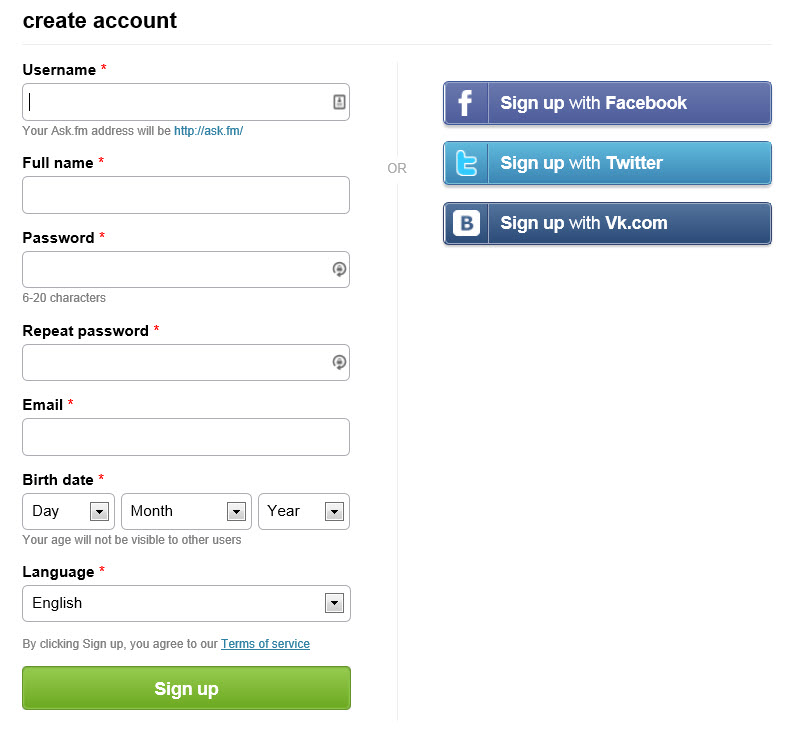
\includegraphics[scale=0.5]{Figures/Chapter2/CreateAccount.jpg}
	\caption{Creating an Ask.fm Account}
	\label{fig:createaccount}
\end{figure}

There is no obvious validation of the user details entered though an account can be linked to the users Facebook, Twitter or Vk.com accounts.

\subsection{Questions and Answers}
Any unanswered questions the user has will appear on their questions page (Figure \ref{fig:questions}). Users will always receive the question of the day and also have the option of receiving a random question if they have not received questions from other users.

\begin{figure}[h!]
	\centering
	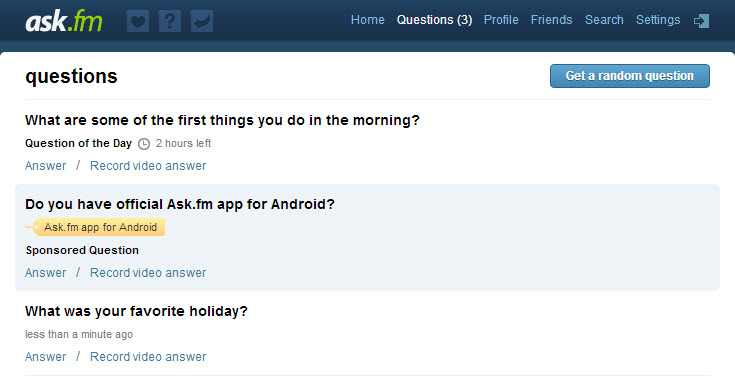
\includegraphics[scale=0.5]{Figures/Chapter2/Questions.jpg}
	\caption{Your Ask.fm Questions}
	\label{fig:questions}
\end{figure}

A question is a maximum of 300 characters long and a question can be asked whether the user has an Ask.fm account or not. Figure \ref{fig:askquestion_01} shows a question being asked by a user who is logged in and notice that the option to ask a question anonymously is also available. It is also possible to ask a question without having an account (Figure \ref{fig:askquestion_02}).

\begin{figure}[h!]
	\centering
	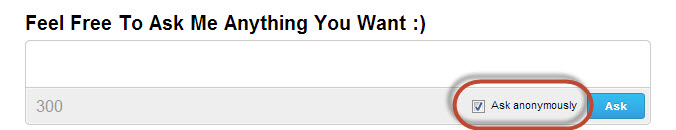
\includegraphics[scale=0.5]{Figures/Chapter2/AskQuestion_01.jpg}
	\caption{Asking a question when logged into your account}
	\label{fig:askquestion_01}
\end{figure}


\begin{figure}[h!]
	\centering
	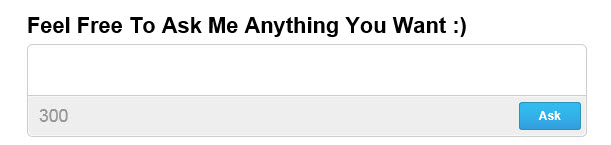
\includegraphics[scale=0.46]{Figures/Chapter2/AskQuestion_02.jpg}
	\caption{Asking a question when not logged into your account}
	\label{fig:askquestion_02}
\end{figure}

Text, a combination of text and a picture (Figure \ref{fig:answer}) or video can be used to answer the question.

\begin{figure}[h!]
	\centering
	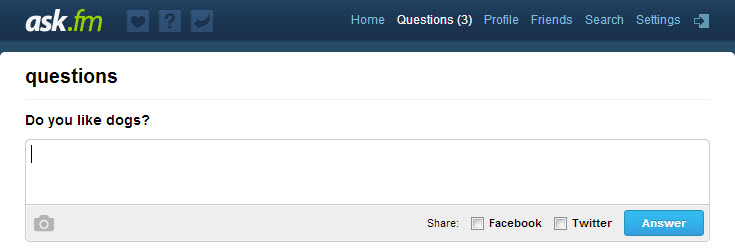
\includegraphics[scale=0.5]{Figures/Chapter2/Answer.jpg}
	\caption{Answering with text and an optional picture}
	\label{fig:answer}
\end{figure}

The option to share an answer using Twitter or Facebook is also available to the user.

\subsection{Privacy Setting, Reporting Abuse and Deleting Questions}
It should be highlighted that it is possible to prevent anonymous questions, to delete offensive questions before they are answered and also to report abuse.

To configure an Ask.fm account so that anonymous questions are not allowed a user can select the ``Do not allow anonymous questions'' on their Settings - Privacy page. On this privacy page it is also possible to select not to display answers on the Ask.fm stream (Figure \ref{fig:privacy}).

\begin{figure}[h!]
	\centering
	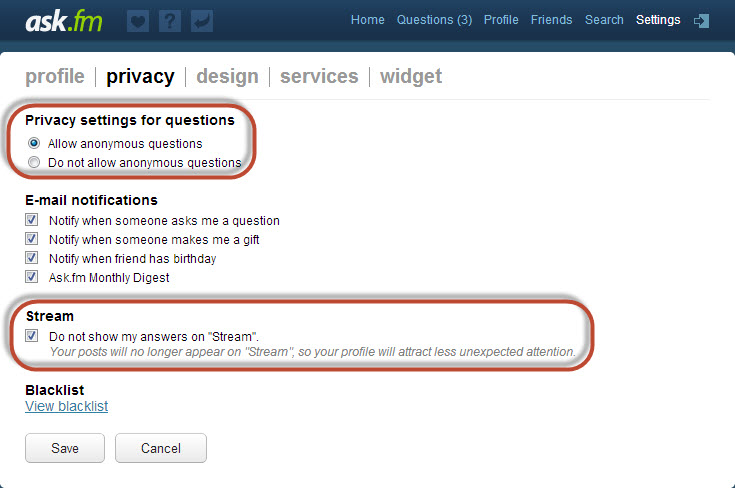
\includegraphics[scale=0.5]{Figures/Chapter2/PrivacySettings.jpg}
	\caption{Configuring privacy settings}
	\label{fig:privacy}
\end{figure}

Both users and questions/answers can be reported. In the top right-hand corner of each question there is a report flag. The option to report a user is available at the top of the users questions and answers page (Figure \ref{fig:report_01}). When the report button is clicked the type of inappropriate behaviour to report can be chosen (Figure \ref{fig:report_02}).

\begin{figure}[h!]
	\centering
	\includegraphics[scale=0.5]{Figures/Chapter2/report_01.jpg}
	\caption{Reporting a user or a question and answer}
	\label{fig:report_01}
\end{figure}


\begin{figure}[h!]
	\centering
	\includegraphics[scale=0.5]{Figures/Chapter2/report_02.jpg}
	\caption{Types of inappropriate behaviours to report}
	\label{fig:report_02}
\end{figure}

It is possible to delete a single question by hovering over the top right-hand side corner of the question where a delete ``X'' icon will appear (Figure \ref{fig:delete}). Alternatively, it is possible to delete all unanswered questions. Finally, it is also possible to block the asker of the question using the ``\textit{Block}'' icon. When a block is requested a new dialogue is displayed requesting the reason this user should be blocked (Figure \ref{fig:block}). This option is presented even when the user has posted anonymously. Blocking a user will cause unanswered question from this user to be deleted. 

\begin{figure}[h!]
	\centering
	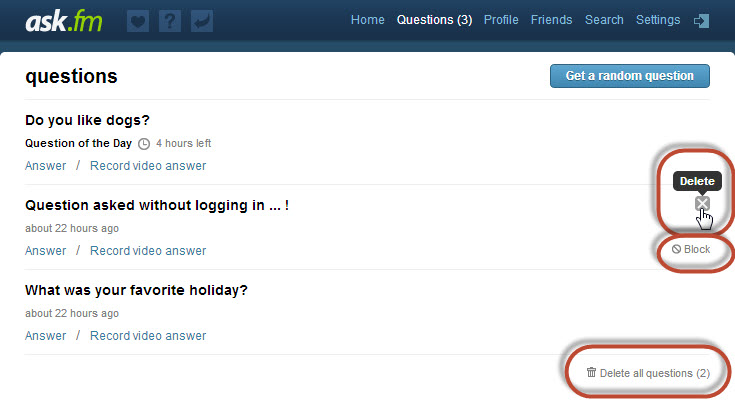
\includegraphics[scale=0.5]{Figures/Chapter2/DeleteQuestion.jpg}
	\caption{Deleting questions and blocking the user that asked the question}
	\label{fig:delete}
\end{figure}


\begin{figure}[h!]
	\centering
	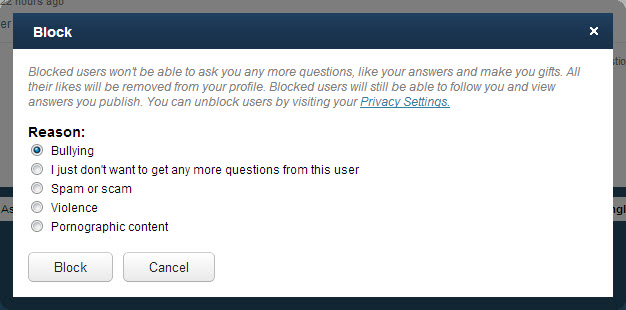
\includegraphics[scale=0.5]{Figures/Chapter2/Block.jpg}
	\caption{Blocking a user to prevent them asking further questions}
	\label{fig:block}
\end{figure}

\subsection{Deactivating an Account}
Finally, it is possible to deactivate an Ask.fm account from the users \textit{Settings - Profile} page but the account can be reactivated at any time.

\begin{figure}[h!]
	\centering
	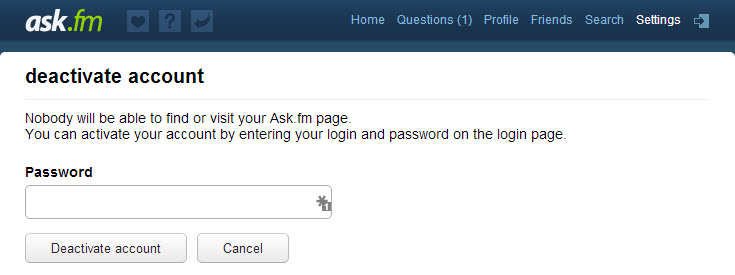
\includegraphics[scale=0.5]{Figures/Chapter2/Deactivate.jpg}
	\caption{Deactivating an account}
	\label{fig:deactivate}
\end{figure}
\section{Python, NLTK and Scikit-Learn}
\label{section:2.2}

In this section Python, the Natural Language Toolkit (NLTK) and Scikit-Learn are introduced. Python is the primary tool used to extract, manipulate and process the datasets used in this research. NLTK and Scikit-Learn are the packages that will generate the classifiers used to predict if a sample is either bullying or not bullying.

\subsection{Python}

Python is an open source high-level programming language developed under an OSI approved open source license. Although considered an excellent choice for the user who is only starting to learn how to program, Python offers enough features and functionality to meet the demands of the professional object-oriented programmer as well. It is highly scalable, portable, embeddable and suitable for development projects of all sizes. Another great advantage of Python is a very active community that enthusiastically develops, releases and supports commercial quality libraries, packages, tools and platforms that enhance and extend the core Python capabilities. Two of these, NLTK and Scikit-Learn are extensively used in this research project. 

Python is extensively used at one of the worlds largest internet company, Google, where it used in the Google App Engine and YouTube to name but a few \cite{google_python}. Currently, there are two main versions of Python supported, version 2.7.8 and version 3.4. Instructions how to download, install and configure Python can be found on the Python Language homepage \cite{python}.

\subsection{The Natural Language Toolkit}

The Natural Language Toolkit (NLTK) is a leading platform for building Python programs to work with human language data \cite{nltk}. The NLTK provides a suite of libraries to handle text processing tasks such as corpora parsing, tokenisation, stemming and classification. The NLTK also provides libraries that support part of speech tagging, which converts a sentence into a list of word / tag tuples, and chunk extraction that can be used to extract a short phrase from a sentence that has previously been part of speech tagged. The NLTK also provides easy access to WordNet \cite{miller_wordnet:_1995}, a large lexical database of English nouns, verbs, adjectives and adverbs, and  access to over 50 corpora.

Like Python the NLTK is a free, open source project. It is community driven and is available for Linux, Windows and Mac OS machines. It is currently based on Python version 2.7 but support for version 3 of Python in planned.

\subsection{Scikit-Learn}

Scikit-Learn is a simple and efficient tool for data mining, data analysis and machine learning in Python \cite{scikit-learn}. It utilises other Python libraries such as NumPy, SciPy, and Matplotlib. Like Python and the NLTK, it is open source available under a BSD license. Scikit-Learn includes many supervised learning algorithms including Naive Bayes, Support Vector Machines, Random Forests and Decision Trees as well as many unsupervised learning techniques including clustering and hidden Markov models. As well as supporting cross-validation and providing comprehensive grid search capabilities for parameter optimization, Scikit-Learn also provides extensive model evaluation metrics and scoring options including, for example, precision, recall and accuracy as well easily accessible confusion matrices. Feature extraction including TF-IDF is also supported.

\subsection{Python Resources}

While writing this research thesis the following books provided invaluable support:

\begin{itemize}

	\item Think Python \cite{downey_think_2012}
	\item Python Text Processing with NLTK 2.0 Cookbook \cite{perkins_python_2010}
	\item Learning scikit-learn: Machine Learning in Python \cite{garreta_learning_2013}
	\item Building Machine Learning Systems with Python \cite{Riegel:2013}

\end{itemize} 

\section{MySQL, SPSS and Excel}

MySQL, SPSS and Excel are other tools that were used to a lesser degree throughout the course of this research project.

MySQL is one of the world's most popular open source database. It was used to house the question records from the Ask.fm site before writing the data to disk in NLTK corpora format. SPSS is predictive analytics software from IBM. It includes a lot of tooling to allow the elegant manipulation of textual data including stratified sampling which was made use of in Chapter \ref{chapter4}. Excel is a spreadsheet package from Microsoft that was used to generate all the charts seen in this dissertation.












\section{Precision, Recall, Accuracy and G-Performance}
\label{section:2.3}

When evaluating the performance of a model in predicting whether a question was correctly classified as bullying or not precision, recall and accuracy will be used. When predicting whether a question is bullying there are four possible outcomes:

\begin{enumerate}

	\item \textbf{True Positive} (TP)\\
	A true positive is where the question is predicted as bullying and was also classified as bullying
	\item \textbf{False Positive} (FP) \\
	A false positive is where the question is predicted as bullying but was also classified as not bullying
	\item \textbf{False Negative} (FN)\\
	A false negative is where the question is predicted as not bullying but was also classified as bullying
	\item \textbf{True Negative} (TN)\\
	A true negative is where the question is predicted as not bullying and was also classified as not bullying

\end{enumerate}

The overall accuracy of a model is calculated as:
\begin{equation}
     \frac{Number of True Positives + Number of True Negatives}{Total Number of Examples}
\end{equation}

Positive Class Precision is calculated as:
\begin{equation}
     \frac{Number of True Positives}{Number of True Positives + Number of False Positives}
\end{equation}

Positive Class Recall is calculated as:
\begin{equation}
     \frac{Number of True Positives}{Number of True Positives + Number of False Negatives}
\end{equation} 

Negative Class Precision is calculated as:
\begin{equation}
     \frac{Number of True Negatives}{Number of True Negatives + Number of False Negatives}
\end{equation}

Negative Class Recall is calculated as:
\begin{equation}
     \frac{Number of True Negatives}{Number of True Negatives + Number of False Positives}
\end{equation} 


Precision and recall are inversely related meaning that as precision increases recall decreases and inversely where recall increases precision decreases. When developing a classification model the critical decision is whether to seek to have high precision and low recall or to develop a model that delivers a low precision value but has high recall. Consider a scenario where we are trying to classify questions as bullying. High precision and low recall values suggest that a high percentage of questions predicted as bullying will be bullying. However, a significant number of bullying questions will not be correctly identified. A high recall value implies that a large percentage of bullying questions have been correctly identified but, as a consequence, a large number of not bullying questions would also be incorrectly identified as bullying yielding low precision. Usually a trade-off has to be made between precision and recall depending on the situation and the preferred outcomes.

\subsection{G-Performance}
In addition to standard classifier performance measures, for example accuracy, precision, recall and F-Measure \citeauthor{kubat_addressing_1997} \cite{kubat_addressing_1997} describes another measure that uses the geometric mean of the accuracies measured separately on each class called the g-performance. The goal of this measure is to maximise the recall of both class but at the same time keeping them balanced such that a poor value for either the positive or negative class will give an overall poor performance for the classifier.

G-Performance is calculated as:
\begin{equation}
     g =\sqrt{\frac{True Positives}{True Positives + False Negatives} \cdot \frac{True Negatives}{True Negatives + False Positives}}
\end{equation} 

%-------------------------------------
%	CHAPTER 3
%-------------------------------------
% Chapter Template

\chapter{Literature Review} % Main chapter title

\label{chapter3} % Change X to a consecutive number; for referencing this chapter elsewhere, use \ref{ChapterX}

\lhead{Chapter 3. \emph{Literature Review}} % Change X to a consecutive number; this is for the header on each page - perhaps a shortened title

The primary focus of this research paper is the automated detection of cyberbullying using tools, techniques and processes from the world of text mining. However, before delving into the details of the approaches that could be used, and the issues presented by this task, it is important to understand cyberbullying and the adverse affects it has on the adolescents and teenagers of today. 
\section{Cyberbullying: What is it and why should we care}
\label{section:3.1}

According to \citet{nahar_step_2013} bullying has moved out of the school yard and is now causing concern online as cyberbullying. \citet{dadvar_improved_2012} highlight that in this age of digital communications you can have hundreds of virtual friends having never met them face to face. \citet{kontostathis_detecting_2013} suggest that the internet and social media applications are being used, particularly by children and teenagers, as a new way to bully, to cyberbully.
 
We begin this review of the literature with an attempt to understand the phenomenon known as cyberbullying. The psychology of bullying and cyberbullying is well-covered elsewhere and is not within the scope of this paper. However, as the principal area targeted by this research is the automatic detection of cyberbullying, it is important first to understand how this new form of bullying is enacted on its victims and then also consider the impact of it on the victims.

The United States Department of Health and Human Services (DOH) \cite{DOH} highlights that bullying exists where there is either a perceived or actual imbalance of power and there is repeated aggressive behaviour. These behaviours could be verbal, for example teasing or name calling, social, including spreading rumours and exclusionary acts or threatened or actual physical violence. \citet{xu_fast_2012} concur with these descriptions of face to face encounters as being what \citet{dadvar_improved_2012} refer to as traditional bullying. Citing the work of others \cite{archer_integrated_2005} \cite{little_disentangling_2003} \cite{nylund_subtypes_2007} bullying is described as taking many forms but the most common are physical or direct aggression, indirect aggressions like name calling and relational or social aggressions such as exclusion. \citet{xu_fast_2012} also highlights that this bullying can be more than an isolated single event and the intended victim can be repeatedly subjected to the abusive behaviour over time.

The DOH describes cyberbullying as bullying using communication tools such as instant messaging, chat sites and social networks using smart phones, computers or tablets. The DOH also highlights that cyberbullying can't be easily turned off and can happen twenty four hours a day seven days a week. To further exasperate the situation the bullying messages or texts can rapidly spread to a large on-line community. Also, the bully can be anonymous and difficult to trace and completely purging the internet of the offending text or image is next to impossible. The persistent nature of the world wide web and functionality provided by social media sites means that these abusive posts can quickly spread amongst a group and can subsequently be accessed again and again by both the victim and the perpetrator \cite{dadvar_improved_2012} \cite{nahar_effective_2013} \cite{dadvar_towards_2012}. The implications of this is that the offending text or image can continuously reappear causing distress to the victim again and again. The effect of the cyberbullying can be traumatic on the victim leading to trouble sleeping, withdrawing from society, stress and more troubling mental health problems like anxiety, depression and suicidal thoughts. 

The DOH is not alone in their views, there is much support for their views and opinions. For example \citet{dadvar_improving_2013} and \citet{nahar_effective_2013} are both of the opinion that cyberbullying is an electronic act, aggressive in nature, against a victim who is typically unable to defend themselves. \citet{dinakar_modeling_2011} and \citet{rybnicek_facebook_2013} describes these electronic acts as images or text messages posted to social media sites with the sole intent of hurting or embarrassing the victim through these repeated offensive postings. 

It is also important to consider the tone and content of a cyberbullying incident and the various forms that it may take. Apart from the threat of physical violence, or the wishing harm on a person,  \citet{dinakar_common_2012} describe three main categorises of cyberbullying as sexual, racial and direct attacks against a person. Sexist attacks are typically against women or sexual minorities such as gay, lesbian, bi-sexual and transsexual individuals and groups. Racial or cultural attacks are typically against a cultural minority and its traditions. Direct personal cyberbullying attacks a persons intelligence or physical appearance for example their weight, height, appearance or IQ. 

\citet{chen_detecting_2012} describes cyberbullying as communications that disparage an individual or group on the basis of their nationality, ethnicity, colour or race, their gender, sexual orientation or religion. \citet{xu_learning_2012} also includes socio-economic status as a cyberbullying category under which the victim can be targeted. \citet{willard_cyberbullying_2006} \cite{willard_cyberbullying_2007} describes the many forms a cyberbullying attack can take as harassment, flaming, outing, exclusion, flooding, cyberstalking, impersonation or masquerading, trolling and denigration of their victims by the bullies. \citet{ptaszynski_michal_machine_2010} bring to our attention and initiative from the Ministry of Education, Culture, Sports, Science and Technology (MEXT) in Japan. Following several tragic suicides attributed to cyberbullying MEXT developed a manual to assist school teachers to identify cases of cyberbullying \cite{ministry_of_education_culture_sports_science_and_technology_netto_2008}. MEXT divided cyberbullying into two separate categories, cyberbullying posts appearing on blogs, forums and private profile sites and cyberbullying emails. These posts and emails can contain libellous or slanderous content, the unauthorised disclosure of sensitive personal data or posts intended to humiliate the victim.

The affects of cyberbullying on its victims can  sometimes have tragic consequences as previously highlighted. News headlines like ``Third suicide in weeks linked to cyberbullying'' \cite{Cionnaith:2102}, ``Cyberbullies claimed lives of Five teens'' \cite{Riegel:2013} and ``Hanna Smith suicide fuels calls for action on Ask.fm cyberbullying'' \cite{laura_smith-spark_hanna_2013} are now, unfortunately, becoming an all too depressingly frequent occurrence. However, behind these eye-catching headlines the daily torment and abuse suffered by the victims of cyberbullying are taking a dire psychological and emotional toll. The negative affects of posts that contain cyberbullying of a personal or sensitive nature can be internalised by children and young adults leading to significant and emotional psychological suffering says \citet{dinakar_modeling_2011}. Apart from suicidal thoughts \citet{xu_fast_2012} say the affects of cyberbullying can include loneliness, anxiety, low self-worth and signs of depression. Other signs described in \citet{xu_learning_2012} are intra-personal problems, school absence or violence and physical complaints.  

In their report ``Cyberbullying Among 9-16 Year Olds in Ireland'' \citet{oneill_cyberbullying_2013} provide an overview of bullying and cyberbullying statistics in Ireland and Europe. The main findings of their report are that nearly one in four (23\%) of all 9-16 year old children had experienced some bullying whether it was on-line or off-line. Although at 4\% the overall number of Irish teens that experienced on-line bullying was lower than the European average of 6\% it was noted that the more ``experienced internet users'', particularly users of internet social media sites, reported higher levels of bullying. The most commonly reported form of cyberbullying was being the target of hurtful or nasty messages. \citet{dadvar_towards_2012}, however, warns that focusing solely on the text of a message may not provide sufficient evidence to conclude that the text is a cyberbullying post. The use of profanities, and what others would consider inappropriate and offensive language, may just be what the protagonists involved consider good banter.

Other types of unacceptable on-line activities that also target adolescents and teenagers include cyberstalking and grooming. \citet{aggarwal_anti-cyberstalking:_2005} define stalking as the unwanted and repeated observation, harassment, intimidation and intrusion of privacy of a person by a predator who wishes to acquire private information about their victim. They continue that the anonymity and wealth of new stalking opportunities offered by the internet has given the stalkers a feeling of relative safety as the technical ability and internet competency of the stalker typically exceeds that of the victim. \citet{rybnicek_facebook_2013} say that the grooming of a child is typically performed by adults who approach children in order to have sexually explicit conversations, to exchange nude photographs or videos or to meet up in person resulting in the sexual abuse of the child. \citet{elzinga_analyzing_2012} say that there are seven stages of grooming. The first two stages are sweet greetings, where pet names like \textit{``sweety''} are used to create an atmosphere of intimacy, and compliments, which is used to strengthen the intimacy sphere by complimenting the targets looks for example. Stages three and four are called intimate parts and sexual handling where the intimate parts or genitalia of the body are introduced to the conversation by using their popular names, for example \textit{``boobs''} or \textit{``willy''}, before the chat becomes more explicit. In stage five the groomer will use photographs and videos to show his private parts and attempt to get the intended victim to do likewise before in stages six and seven the location, where, and the date, when, the groomer can meet the victim is discussed

So how then can modern machine learning and computing help in the detection of cyberbullying? Some of the approaches used in the detection of cyberbullying are further explored next.
\section{Mining for Cyberbullying Text}
\label{section:3.2}

The application of text mining tools, techniques and processes to the automatic detection of cyberbullying text is still a relatively new research area \cite{xu_fast_2012} \cite{xu_learning_2012}. There appears to be a clear trend where text mining approaches are supplemented with other techniques such as the analysis of the social graph of the bully and the victim or by determining the role played by each party in a cyberbullying incident. When training a classifier to identify documents of different types a ``bag of words'' approach is a commonly used method that uses the frequency of the occurrence of each word in a document as a feature used to help determine a documents class. One of the first mentions of a bag of words in this linguistic context was in the 1953 ``Distributional Structure'' paper by \citet{harris54}. The bag of words approach is at the heart of many attempts to automatically detect cyberbullying.

\citet{yin_detection_2009}, in ``Detection of Harassment on Web 2.0'' presents an approach to the detection of harassment that utilises content, sentiment and contextual features of documents. Using the Kongregate, Slashdot and MySpace datasets presented by Fundación Barcelona Media (FBM) for analysis at the CAW 2.0 workshop \cite{fundacion_barcelona_media_fbm_caw_2009}, the goal of this research was the identification of deprecating remarks. Three local features N-Grams, Foul words and Term Frequency - Inverse Document Frequency (TF-IDF) are used and local features are described as features that can be extracted directly from the text of the message. 

N-Grams are a contiguous sequence of n items from an extract of text or speech and in this occurrence the n-grams are words. For example, given a sequence of words ``The quick brown fox'' the following tri-grams, or sequences of three words, can be formed ``The quick brown'' and ``quick brown fox''. TF-IDF is a statistical measure of how important a given word is in a collection of documents. Each document is represented as a vector of words and each word is represented in the vector by a value that is indicative of its importance in predicting the class of the document. The TD-IDF weight for a word \textit{i} in document \textit{j} is given as: 

\begin{align}
	TFID{F}_{{ij}}=T{F}_{{ij}}\cdot ID{F}_{{i}}
\end{align}

Where \textit{TF} is a measure of a words importance in a document and is calculated as:

\begin{align}
	T{F}_{{{\dot{i}}j}}=\frac {{n}_{{ij}}}{{\Sigma }_{{k}}{n}_{{kj}}}
\end{align}

The number of times a word \textit{i} appears in a document \textit{j} is represented by ${{n}_{{ij}}}$ and ${{\Sigma }_{{k}}{n}_{{kj}}}$ is a count of all words in document \textit{j}. This means that the more times a word appears in a document the larger its value for \textit{TF} will get. The \textit{TF} weighting of a word in a document shows its importance within that single document. \textit{IDF} then shows the importance of a word within the entire collection of documents or corpus and is calculated as:

\begin{align}
	ID{F}_{{i}}={log{\frac {\mid{P}\mid}{\mid{\{{{p}_{{j}} \:: \: {t}_{{i}} \: \epsilon \: {p}_{{j}}}\}}\mid}}}
\end{align}

Where $\mid{P}\mid$ is the total number of documents in the corpus or collection and $\mid{\{{{p}_{{j}} \:: \: {t}_{{i}} \: \epsilon \: {p}_{{j}}}\}}\mid$ represents the number of documents in which the word, or term, ${t}_{{i}}$ appears. The nature of the \textit{IDF} value is such that terms which appear in a lot of documents will have a lower score or weight. This means terms that only appear in a single document, or in a small percentage of the documents, will receive a higher score. This higher score makes that word a good discriminator between posts \cite{yin_detection_2009}. 

In their research \citet{yin_detection_2009} used the libSVM \cite{CC01a} learner with a linear kernel as their classification tool with ten-fold cross validation. They found a combination of 1, 2 and 3 n-grams, foul or profane language and TF-IDF on their own did not perform very well. When applied separately to the three datasets F-Measure scores of less then 0.2 for n-grams and foul words and between 0.25 and 0.40 for TF-IDF were returned. When combined with sentiment features and contextual features a small improvement in F-Measure values was seen. When reviewing the dataset it was noticed that a lot of the posts classified as harassment contained foul language used in conjunction with pronouns, particularly second person personal pronouns such as ``you'', ``your'' and ``yourself''. To boost the effectiveness of these pronouns the sentiment features were captured together into three groups. The first group treated all second person pronouns together as a single term. The second group took all other pronouns together as a single term, for example, ``he'', ``she'', ``her'' etc. and the final group treated all foul words as a single term. The TF-IDF weighting of the combined terms was calculated for each group. It was identified, for contextual features, that the posts classified as harassment were ``different'' to their neighbouring posts so a cosine similarity between posts was calculated to assist in the identification of the bullying posts. The authors concluded that combining these sentiment and context feature to the earlier content features lead to an increase in F-Measure values to between approximately 0.3 and 0.44.

In ``Modelling the Detection of Textual Cyberbullying'', \citet{dinakar_modeling_2011}, a set of binary and multi-class classifiers, developed using a bag of words approach, are proposed for the detection of textual cyberbullying in a corpus of 50,000 YouTube comments. Unlike \citet{yin_detection_2009} a set of preprocessing steps were used on the comments including stemming, stop word removal and the removal of repeated characters for example ``lollllll''. Stemming is a process by which  derived or inflected  words are reduced to their stem, sometimes also called the base or root. Using the words stemming and stemmed as examples, these are both based on the word stem. The first algorithm proposed for a stemmer was by \citet{lovins_development_1968} in 1968. When processing natural language, or text, stop words are words which are filtered out of the corpus typically early on in the process \cite{rajaraman_mining_2011}. Stop word are usually what are called short function words or words with little or ambiguous meaning. Example of English stop words include ``the'', ``and'', ``at'', ``which'' etc.  After preprocessing, the YouTube comments were divided into several clusters representing different types of harassment, for example, physical appearance, sexuality, race and cultural and intelligence. From each cluster 1,500 comments were hand-annotated to verify that labels were correctly applied to each cluster. Comments that did not fit in any of the clusters were given a neutral label. Like \citet{yin_detection_2009} some general features of the text were used. Both TF-IDF weighted uni-grams and a list of profane words were used. In addition, the Ortony lexicon \cite{ortony_referential_1987} of words donating negative connotation, the positive words were stripped beforehand, and frequently occurring part of speech (POS) bi-grams were utilised. 

In their experiment set-up \citet{dinakar_modeling_2011} divided their datasets 50\% for training, 30\% for testing and 20\% for validation. A Naive Bayes classifier, as well as three supervised learning methods, were used to train a model. The supervised learner were Support Vector Machines (SVM), J48 which is a C4.5 based decision tree classifier and JRip a propositional rule learner. In the first experiment the models were trained on each dataset separately i.e. a binary classification task. In the second experiment the datasets were combined into a single dataset and the models were trained as a multi-class classifier. Rather than using accuracy alone in the assessment of the performance of the models developed Cohen's kappa statistic was also used. It was found that the binary classifiers developed performed much better than the multi-class classifier. It was also observed that whilst the JRip rule-based model gave the best accuracy with values as high as 80\% the SVM gave the best kappa statistic values ranging from 0.72 to 0.79 for the binary classifiers. \citet{kontostathis_chatcoder:_2009} also utilises the J48 classifier from Weka \cite{hall_weka_2009} when attempting to categorise predators and victims in grooming chat transcripts from Perverted Justice \cite{_perverted-justice.com_????} and ChatTrack \cite{bengel_chattrack:_2004}.

\citet{reynolds_using_2011} explicitly state that they wanted to avoid a bag of words approach. This was because the feature space of the bag of words approach can become very large, they wished to be able to produce the model in code and they wanted to be able to fully understand the reason a post was considered as cyberbullying. Having reached the conclusion that ``bad'' words, for example, swear words, profanities and offensive words, were a good indicator of cyberbullying a weighted dictionary of terms, built from the terms on www.noswearing.com, was generated. The weighting ranged from 100 to 500 depending on the deemed severity of the word. The dataset used was scrapped from the www.formspring.me website, a questions and answers style website, and labelled using Amazon Mechanical Turks. Using the bad word dictionary the contents of each message was then scored in several ways. Two datasets were created and in the first the count of bad words contained in each post, \textit{NUM}, was calculated and in the second a normalised count of the words, \textit{NORM}, was calculated to reflect the density of the bad words in each post. When calculating the normalised value the severity weight of each bad word was also considered. In additional \textit{SUM} and \textit{TOTAL} values were also calculated were SUM is the overall weighted average badness of a post taking into account the severity weighting of each word and TOTAL is the total number of words. In additional to the J48, JRip and SVM learners, which were also used in \cite{dinakar_modeling_2011}, IBK an instance based algorithm was also used. Using ten-fold cross validation the authors report that the NORM dataset outperformed the NUM dataset suggesting that the percentage of bad words in a post is more indicative of cyberbullying than a simple count of bad words. Overall the learners used, with the exception of SVM, were able to correctly identify 78.5\% of cyberbullying posts.

\citet{chen_detecting_2012} presents a two phase Lexical Syntactic Feature (LSF) based framework for the detection of offensive content and users. Their proposed system presents a new method of sentence offensiveness prediction based on the overall offensiveness of the words in the sentence. The offensive is measured using a lexicon constructed using \citet{xu_filtering_2010}, the Urban Dictionary, and a syntactic intensifier that adjusts a words offensiveness based on the context in the sentence. Words defined as being either strongly offensive and given a larger weighting, for example, profanities such as ``fuck''. Weakly offensive words, such as ``stupid'' or ``liar'', were given a smaller weighting. Words that were not offensive were given a neutral weighting. When a pejorative or obscenity is directed at a user, or semantically associated with another pejorative or obscenity, it is suggested that they become more offensive. For example, the word stupid would be considered more offensive when directed at a person, ``are you stupid'', opposed to referring to the latest console game ``it's a stupid game'' giving the word a larger intensifier value. Using this intensifier value the offensive value of a word is adjusted accordingly giving an overall sentence offensive value ${O}_{{s}}$ of:

\begin{align}
	{O}_{{s}}={\sum {{o}_{{w}}{I}_{{w}}}}
\end{align}

The offensiveness of a user is a combination of the aggregate of the sentence's offensiveness and the extraction of some of the users language styles. The dataset used was a corpus of over two million YouTube comments with minimal preprocessing. Six approaches were used to determine each sentence's offensive values including bag of words, 2-gram, 3-gram, 5-gram, an appraisal approach \cite{whitelaw_using_2005} and the newly proposed LSF approach. Recall, precision and F-Score, F-Measure, were used to evaluate each of the approaches. Also of interest to the authors was a measure of false positives, sentences erroneously scored as offensive, and false negatives, sentences that should have been scored as offensive but were not. A summary of how each approach performed is shown in Figure \ref{fig:chen_detecting_2012_01} where the Proposed LSF approach performed the best.

\begin{figure}[htbp]
	\centering
	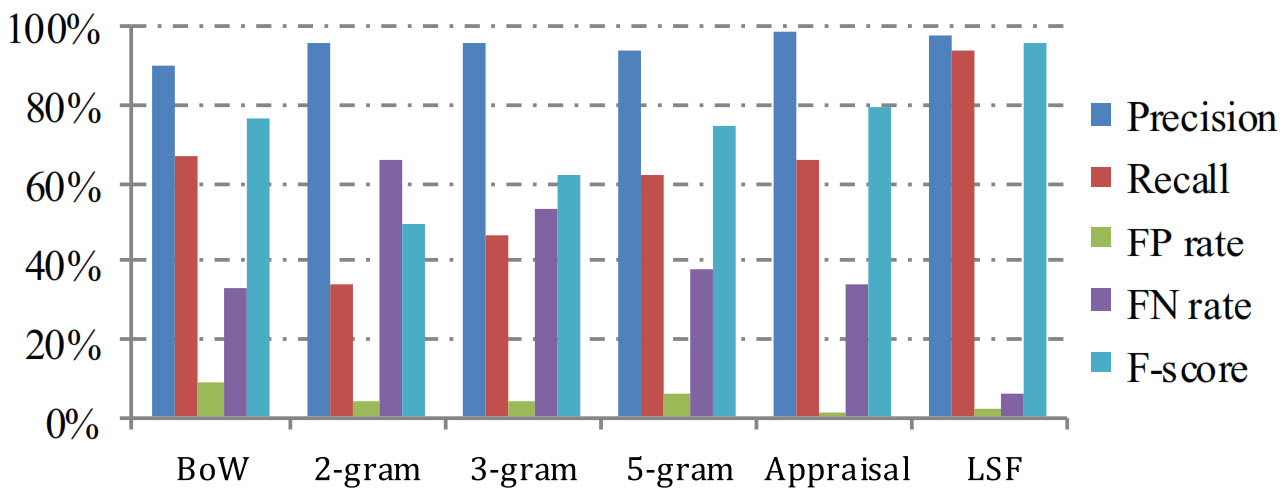
\includegraphics[width=0.75\textwidth]{Figures/Chapter3/chen_detecting_2012_01.jpg}
	\caption[Accuracies of sentence level offensiveness detection]{Accuracies of sentence level offensiveness detection \citet{chen_detecting_2012}}
	\label{fig:chen_detecting_2012_01}
\end{figure}

The calculation of an individual users offensiveness was a more complicated matter. A number of users, whose sentence offensiveness levels as calculated in phase one was uniformly distributed, next had their comments manually annotated as either offensive or not. Using Naive Bayes and SVM classifiers and ten-fold cross validation a number of experiments were then run to determine a user offensiveness estimation. The authors found that using both strongly offensive and weakly offensive words in the calculation achieved better results than the proposed LSH. However, on removing the strongly offensive words LSF proved a better predictor. In both cases, the learner that performed the best was SVM.

Like some of the previous papers reviewed \citet{dadvar_improving_2013} also used the content features of manually annotated comments collected from YouTube as well as cyberbullying features and user based features of the text. However, rather than use a bag of words and a TDIDF approach the numerical values for each feature was calculated. The first two content features used we have seen before. These are the number of profane words, taken from a dictionary of 414 words and the number of first and second person pronouns. Both of these features were normalised on the overall length of the comment. The third feature was a boolean feature called the profanity window which identified where a profanity was within a given window size, for example, two to five words, of a second person pronoun. The fourth feature was a normalised count of the number of emoticons. The final feature was the ratio of capital letters in the comment, to capture perceived shouting.  The cyberbullying features were the normalised number of bullying words based on a manually compiled dictionary of bullying words and also the length of the comment. It was proposed that bullying comments are typically shorter in length than not bullying comments. The final group of features used are user features. To exploit the knowledge already known about each user their historical content features were averaged to determine if there was a history of offensive language use. All the content features listed were considered in this calculation as well as the users age. Before processing stop word removal and stemming was applied. A SVM was used to classify the comments and precision, recall and F-Measure values were used to rate the performance of the model. The content based features were first used on their own to obtain a baseline. The content based features get an F-Measure value of 0.55. Next the cyberbullying features were also included and their inclusion saw an increase in the F-Measure value to 0.60. The user features were then added and this resulted in an F-Measure value of 0.64 which led the authors to conclude that the inclusion of user features lead to an increase in the detection of cyberbullying accuracy.

\citet{xu_learning_2012} say that the computational study of cyberbullying is, except for a few exceptions, largely unexplored. Using simple logic based on manual inspection of a Twitter dataset they calculate that there are probably upwards of 50,000 English bullying tweets a day. They outline three approaches that could be used in the detection of cyberbullying. The first is a Natural Language Processing (NLP) task which uses a sample dataset of tweets that has been keyword filtered to contain the terms ``bully'', ``bullied'' and ``bullying''. 1,762 sample tweets were hand annotated and no pre-processing, such as stop word removal or stemming, was performed but the data was case folded \cite{settles_closing_2011}, user names were anonymised, and URLs were replaced with the ``HYPERLINK'' token. Emoticons and Hashtags were also treated as tokens. Following this processing three feature representations, uni-grams (1g), uni-grams and bi-grams(1g2g) and part of speech (POS) coloured uni-grams and bi-grams (1g2gPOS) were created. Four common text classifiers, Näive Bayes, SVM with linear kernel, SVM with RBF kernel and Logistic Regression, were trained on dataset sizes ranging from 100 to 1,500 tweet and then tested using tweets that were held back. Although SVM(linear) + 1g2gPOS achieved an accuracy of 81.6\%  it was decided that SVM(linear) + 1g2g, 81.3\% accuracy on the training data and F-measure 0.77 on the test data, was preferred due to its simplicity. Of all the classifiers used, Naive Bayes performed the worst.

The second approach suggested by \citet{xu_learning_2012} is based around the role a user takes in a cyberbullying incident. These roles, and their relationship, is shown in Figure \ref{fig:xu_learning_2012_01}:

\begin{figure}[htbp]
	\centering
	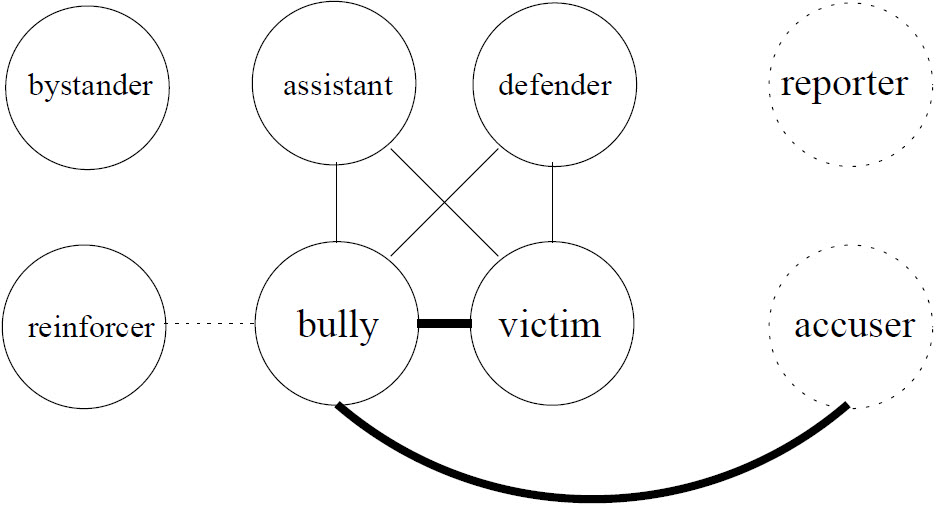
\includegraphics[width=0.75\textwidth]{Figures/Chapter3/xu_learning_2012_01.jpg}
	\caption[Roles taken in a cyberbullying incident]{Roles taken in a cyberbullying incident \citet{xu_learning_2012}}
	\label{fig:xu_learning_2012_01}
\end{figure}

The role taken by the bully and the victim are apparent and need not be examined further. The bullying role is supported by the assistant role and reinforcer role. Though they did not start the bullying the assistant joins in and adds further bullying comments The reinforcer is seen to approve, maybe by liking the bully's post, but does not directly join in. The defender, reporter and accuser roles support the victim. The defender will stand up for the victim, maybe by adding positive comments and also by standing up for the victim. The accuser, however, will go a step further and might confront the bully about the offending comment and point out that they are bullying the victim. The reporter brings the bullying content to the attention of a parent or other authoritative figure. The bystander sees the post and does nothing. The primary interaction is between the bully and the victim but the strength of the line from the accuser to bully is indicative that the confrontation of the bully by the accuser is equally important. 

Four of the most frequently observed roles are targeted Accuser (A), Bully (B), Reporter (R) and Victim (V). The other roles were merged into a single generic role of Other (O). Two tasks were then defined. The first is to identify the author of the tweet which is held in an AUTHOR token. The second is to label each person mentioned in the tweet with one of the bullying roles. Following a manual annotation exercise and using the same classifiers and training techniques as before SVM(linear) + 1g2g gave the best results in the first task. The second task compared the performance of a Conditional Random Field (CRF) classifier against the SVM(linear) to correctly identify the various roles. Once again the data was manually annotated and it was found that for this task the CRF outperformed SVM with an accuracy of 87\% and an overall F-Measure of 47\%. It was discussed that the performance values for precision and recall were low because the tweets were short in length and considered noisy.

Sentiment analysis was the next task undertaken. It was decided to focus on whether a tweet, previously identified as bullying, could be considered as teasing. Hand annotating the tweets from the initial text categorisation task and using the same feature representations and classifiers SVM(linear) + 1g2g again gave the best accuracy performance of 89\%. However, overall, nearly half of the teasing example were misclassified. The lack of emoticons or tokens, and the inconsistency of their use, where they are used indiscriminately in both bullying and not bullying tweets was suggested as a possible reason why the overall performance was poor. Another reason suggested was the lack of standardisation in the spelling of the token or the representation of the emoticon.  

Finally in an effort to understand the main topics from the cyberbullying tweets a collapsed Gibbs sampling implementation of Latent Dirichlet Allocation (LDA) \cite{griffiths_finding_2004} was run. Six topics of interest highlighted by the authors are feelings, suicide, family, school, verbal bullying and physical bullying.


A novel approach to the detection of cyberbullying by using gender information is suggested by \citet{dadvar_improved_2012} . Referring to work by \citet{argamon_gender_2003} and \citet{chisholm_cyberspace_2006} the authors investigated the differing bullying vocabularies of males, who tend to use profanities and threatening behaviour, and females, who use a more relational aggression such as social exclusion or by ganging up on an individual. This was shown to be true as seen in Figure \ref{fig:dadvar_improved_2012_01}. Using supervised learning on a corpus where the gender of the author was known, the dataset was separated into male and female subsets and the features of each set of posts are extracted. Profane words are treated by calculating their ratio in each post and then normalising. Second person pronouns are again considered important and treated separately to all other pronouns. A TF-IDF of all the words in the post was also calculated. The authors of the paper found that incorporating gender specific features achieved better overall detection accuracy with a 39\% increase in precision, 6\% increase in recall and 15\% improvement in the F-Measure.


\begin{figure}[htbp]
	\centering
	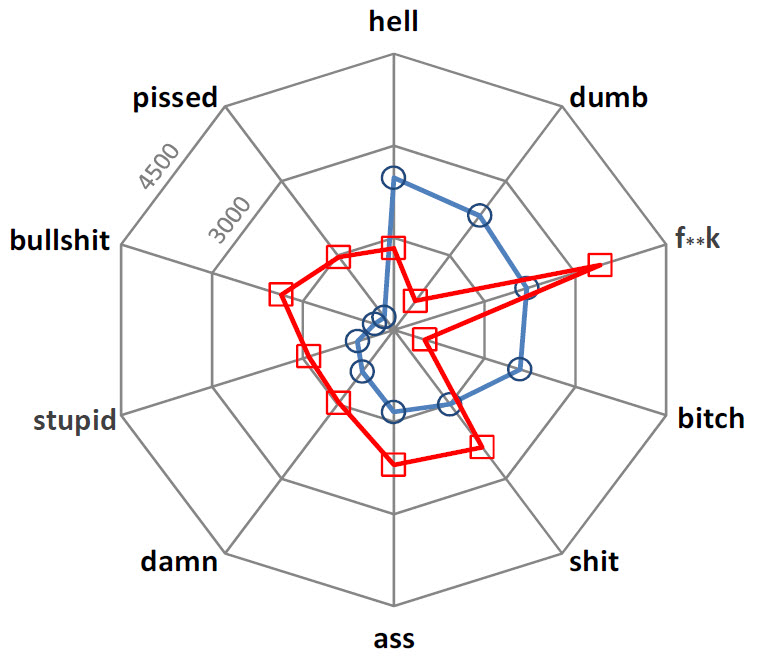
\includegraphics[width=0.75\textwidth]{Figures/Chapter3/dadvar_improved_2012_01.jpg}
	\caption[Top ten profane words for male and female authors]{Top ten profane words for male (square) and female (circle) authors \citet{dadvar_improved_2012}}
	\label{fig:dadvar_improved_2012_01}
\end{figure}
 

\citet{nahar_effective_2013} suggests a two phase approach  to identify cyberbullying instigators and victims by graphing the cyberbullying network and by using a ranking algorithm. In phase one harmful messages are detected using a weighted TF-IDF scheme on bullying features, like a bad word dictionary, and an LDA topic modelling approach which, as previously seen, can be used to understand the underlying semantic topics (for example bullying). The second phase involves building a weight directed graph model of the users social networks to determine who the victims are and who the predators are. Each user is given a predator and victim rank based on the number of harmful messages sent or received. A predator is a user that sends messages with harmful words to users with a higher victim score, a victim is a user that receives messages from users with higher predator scores. Using the users predator and victim ranking in conjunction with the message analysis results from the first phase it was possible to more accurately predict real instances of cyberbullying. Figure \ref{fig:nahar_effective_2013_01} shows an example weighted graph where \textit{u1} has been identified as a predator and \textit{u2} a victim based on the number of harmful messages sent or received.

\begin{figure}[htbp]
	\centering
	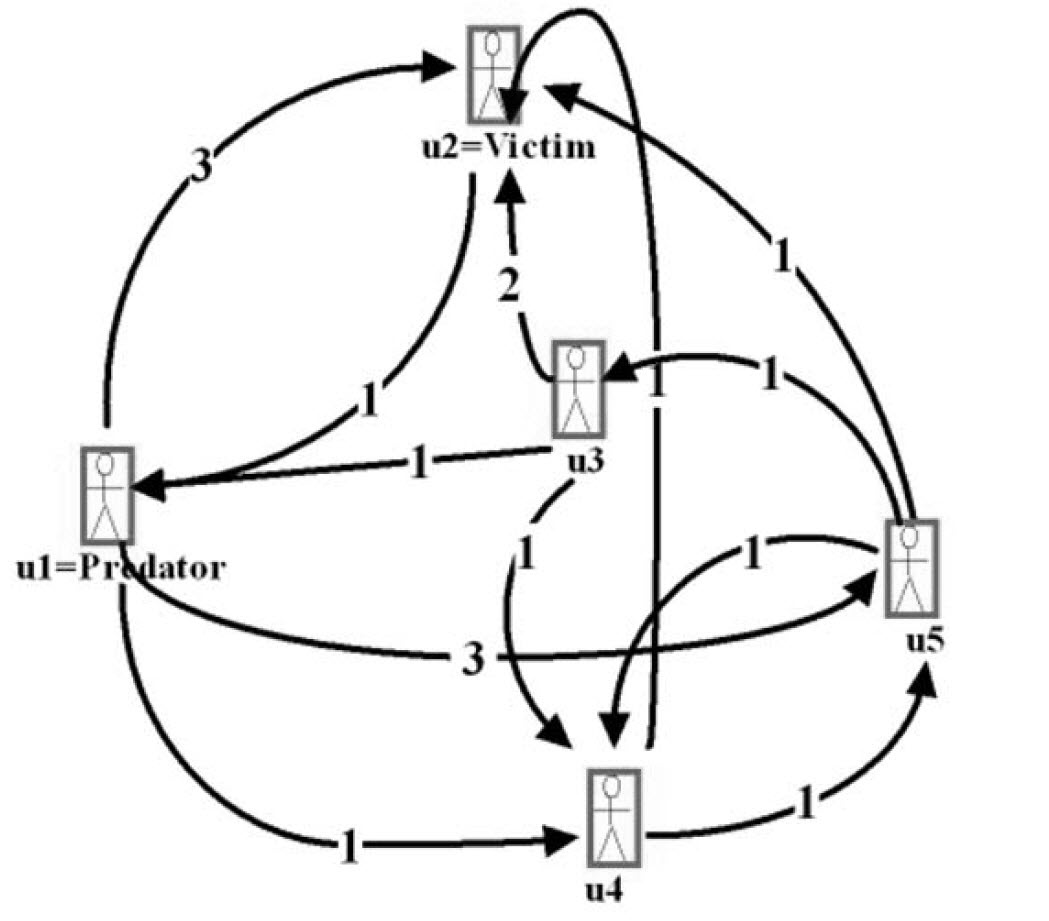
\includegraphics[width=0.75\textwidth]{Figures/Chapter3/nahar_effective_2013_01.jpg}
	\caption[Weighted graph model identifying predators and victims]{Weighted graph model identifying predators and victims \citet{nahar_effective_2013}}
	\label{fig:nahar_effective_2013_01}
\end{figure}

The corpora used were the FBM MySpace, Kongregate and Slashdot datasets from CAW 2009 \cite{fundacion_barcelona_media_fbm_caw_2009}. The data was deemed to be noisy and was preprocessed to increase the quality and the effectiveness of the analytical steps. The text was converted to lower case then stemming and stop words removal was applied before hyperlinks and extra characters were removed. As seen in other works, three types of semantic features, all second person pronouns, all other pronouns and foul words were defined. A weighted TF-IDF scheme was used with the foul words weighted by a factor by two. Finally, an LDA model was used, and the top features generated were selected. The words generated under the bullying, and not bullying topics were extracted and ranked. A linear kernel SVM classifier was used to generate the model. The weighted TF-IDF results were compared against the previous research baseline values, by the same authors \cite{nahar_sentiment_2012}, and also against the LDA features. The weighted TF-IDF outperformed the baseline significantly. On the Slashdot an MySpace datasets it was nearly by a factor of three with an F-Measures of 0.30 and 0.31 for the former and 0.87 and 0.92 for the latter.  Overall it was considered that weighted TF-IDF outperformed all other methods.

The final paper to be reviewed in this section was \citet{kontostathis_detecting_2013} where a number of experiments are performed to identify terms that are indicative of cyberbullying. The dataset used was one that was manually scrapped from the www.formspring.me social media site where users interact using a question and answer model. The dataset was labelled using the Amazon Mechanical Turk service with posts identified as cyberbullying labelled as yes and not bullying posts labelled as no. Approximately 11\% of posts, or 1,185 out of 10,685, were identified as containing content that could be considered cyberbullying. The first experiments utilised a bag of words approach that the authors consider as simple and transparent. The only pre-processing performed was the conversion of all letters to lower case and the removal of all numeric characters and special characters. It was identified that this could lead to the loss of the emphasis as capital letters can be used to show displeasure. The removal of the special characters would also lead to emoticons being removed which are used to show emotions. No other pre-processing was performed giving 15,713 unique terms which gave a term by document matrix of 10,685 x 15,713 where the intersection of rows and columns represented the number of times a term appeared in a particular post. As discussed previously it was determined that ``bad'' words are a likely predictor of cyberbullying. A dictionary of bad words was constructed using the terms on the www.noswearing.com website. Each term in the bad word dictionary was then used to query the 10,685 posts returning the number of times each word appears in each post. After all the words in the dictionary had been queried any posts that returned zero bad words were discarded. The remaining posts were sorted by their overall bad word occurrence count. The number of true positive posts in the top 10, 20, 30, 100 and 500 sorted posts was also noted to identify the terms that yielded the highest top  scores. Another similar round of context based experiments was also run using the 1,185 identified bullying posts. 

The outcome from the first set of queries was to assist in developing another set of query terms that could be used to predict cyberbullying. Precision, recall and f-measure were used to determine the performance of this first set of queries. The result of this analysis was four groups of terms from the bad word dictionary. The first set of words were representative of the terms that results in a precision value of greater than 0.75 and it was found that twenty five terms met this criteria. The next group was made up of 39 terms that achieved a true positive rate for recall of greater than 0.50. The third group of term were representative of words that had at least five posts in the top ten list of posts when sorted by bad word rating of which there were 48 terms. The final content based group consisted of all the terms in the bad word dictionary. A similar analysis was performed on the results of the context queries. There were seven posts with a precision of greater than 0.75 and the words from these posts were used to form the first context based group of words. The second group of context based words was made up of the terms in the top ten queries that had the highest number of true positives. the final context group contained the words of posts that had at least nine true positives in the top ten ranked documents. These four content based and three context based queries were then run against the data and their results were analysed. The authors found that the bad words content queries, F-Measure 0.49 to 0.57, outperformed the context queries, F-Measure 0.28 - 0.45, even though the context queries contained helper and filler words which it was assumed would help. Whilst it was found that precision values were high, recall values did suffer and while the longer content based queries were effective this was at the cost of performance.

This completes the review of approaches that can be used to mine text posted on social network sites for cyberbullying content. During the course of this review it was clear that a number of issues or obstacles reappeared again and again throughout all the papers reviewed. The next section will give a brief overview of these issues and some of the suggested solutions. The topics covered include anonymity, the availability of suitable datasets, classification or labelling and handling class imbalance.

\section{Common Obstacles to Overcome}
\label{section:3.3}

It was mentioned at the end of the previous section that a number of issues or obstacles reappeared again and again throughout the literature review. This next section will give a brief overview of these issues and, where offered, some of the suggested solutions. The topics include anonymity, the availability of suitable datasets, classification or labelling, and class imbalance.

\subsection{Anonymity}

\citet{dinakar_modeling_2011} identifies that the ability to anonymously post hurtful content online that targets another person and the absence of meaningful supervision of the electronic medium as two of the factors contributing to the increasing social menace of cyberbullying. \citet{yin_detection_2009} suggests that the anonymity offered in on-line communities gives the bully the perception of a ``safer'' environment where their real identity is hidden implying that they are free to bully without fear of discovery. \citet{nahar_effective_2013} highlights that an anonymous cyberbullying post can create a heightened sense of fear in the victim as they are confronted with the unknown. The anonymity gives the bully a feeling of power and control over their victim. \citet{reynolds_using_2011} and \citet{kontostathis_detecting_2013} both agree that www.formstring.me, a questions and answers format social media site, which permits the posting of an anonymous question to a user of the site, is prone to cyberbullying because of this offer of anonymity. One interesting solution to the anonymous posting of content online, the Real Name Verification Law, is described in \citet{cho_empirical_2012}. This law, introduced in South Korea in 2007, meant that before users could post on popular sites they first had to verify their real name. The Real Name Verification Law was overturned in 2012 \cite{sang-hun_south_2012}.

\subsection{Data and Classification}

Nearly every major paper reviewed expressed frustration at the lack of a standard labelled dataset that could be used in the research of cyberbullying detection. \citet{yin_detection_2009} and \citet{nahar_effective_2013} both used the MySpace, Kongragate and Slashdot datasets from Fundación Barcelona Media datasets provided for the CAW 2.0 Workshop \cite{fundacion_barcelona_media_fbm_caw_2009}. \citet{nahar_effective_2013} also used the manually labelled dataset from \citet{yin_detection_2009} as their ground truth. \citet{dinakar_modeling_2011} used comments from YouTube videos as their data, treating each comment as a stand-alone comment. \citet{dadvar_improving_2013} also used YouTube video comments but \citet{xu_fast_2012} and \citet{xu_learning_2012} used Twitter tweets as their dataset.  \citet{kontostathis_detecting_2013} and \citet{reynolds_using_2011} both used data that was scraped from the www.formspring.me website.

Once the data had been acquired the next issue was the classification or labelling of the data to identify those posts which were considered to contain cyberbullying content and posts that did not. In most cases, the data was manually classified using a simple binary label \cite{dadvar_towards_2012} \cite{dadvar_improving_2013}  \cite{dinakar_modeling_2011} \cite{yin_detection_2009} by annotators known to the authors but the Mechanical Turk service offered by Amazon was also used on occasion  \cite{kontostathis_detecting_2013} \cite{reynolds_using_2011}. \citet{xu_fast_2012} and \citet{xu_learning_2012} used Twitter tweets for their dataset and rather than classifying by hand an enriched dataset was created by automatically filtering on tweets that contained the ``bully'', ``bullying'' and ``bullied'' keywords. In \citet{chen_detecting_2012} a semi-automated process was used where words were automatically identified as profane using a dictionary and weighted according to their offensiveness.

\subsection{Class Imbalance}

It was also recognised that there existed a class imbalance between the positive bullying class, and the negative class \cite{dadvar_towards_2012} \cite{chen_detecting_2012}. \citet{reynolds_using_2011} found that only 7.2\% of their training dataset was given a positive classification. As a result of this imbalance, it was observed that the chosen learner could achieve accuracy figures of over 90\% by ignoring the cyberbullying cases and by just labelling everything as not containing cyberbullying. \citet{yin_detection_2009} and \citet{reynolds_using_2011} address this issue by replicating the positive classes.

\citet{weiss_cost-sensitive_2007} suggests that most classifiers are designed to maximise accuracy implying that when used to label a highly imbalanced dataset the more frequently occurring class will be predicted. However, when labelling such a highly skewed dataset it is usually the case that it is the less frequently occurring class that is of interest, for example in medical diagnostics and fraud detection. Three methods were evaluated to handle class imbalance. The first method uses  Randon Under Sampling (RUS) or the majority class. The second uses Random Over Sampling (ROS) of the minority class. The third method is a cost based method where the cost of misclassification is built into the learner. Under and over sampling are not without their disadvantages. Under sampling runs the risk of discarding potentially useful data whilst over sampling, besides increasing the learning time required, can lead to over fitting or the generation of a rule specifically for the replicated data. In their experiments a number of datasets were used with the C5.0 cost sensitive decision tree learner \cite{rulequest_research_data_2013},  an enhanced version of C4.5 \cite{quinlan_c4.5:_1993} learner. For the experiments, the unbalanced datasets were submitted to the C5.0 learner with a variety of costs for misclassification. Each dataset was then rebalanced using both over and under sampling to replicate a ratio that mimicked the cost of misclassification and submitted to the C5.0 learner without a cost. Though the overall result was inconclusive, by measuring the total cost of misclassification at the various costs / ratios it was found that for larger datasets, greater than 10,000 examples, the cost sensitive algorithm outperformed both over and under sampling methods. Over sampling was found to perform the best on smaller datasets, in the experiments this was on datasets of less than 250 examples.

\citet{kubat_addressing_1997} refers to the problem when one dataset is significantly larger than the other as ``Addressing the Curse of Imbalanced Training Sets''. They identify that it is usually the minority class that is of interest and point out that a classifier that achieves 99.8\% accuracy where the minority positive class only consists of 0.2\% of the samples is, in fact, of no use at all if it the presence of the samples of interest are completely ignored. In addition to standard classifier performance measures, for example accuracy, precision, recall and F-Measure \citeauthor{kubat_addressing_1997} describe another measure that uses the geometric mean of the accuracies measured separately on each class as $g =\sqrt{\frac{TP}{TP + FN} \cdot \frac{TN}{TN + FP}}$. The goal of this measure is to maximise the accuracies of both classes but at the same time keeping them balanced such that a poor value for either the positive, or negative class, will give an overall poor performance for the classifier.

There are other papers that suggest alternative approaches to tackle class imbalances. \citet{chawla_smote:_2002} uses a combination of under sampling of the majority class and over sampling of the minority class using their novel algorithm SMOTE, Synthetic Minority Over-sampling Technique, to create synthetic minority class examples.\citet{cardie_improving_1997} presents two case based learning frameworks in a natural language environment that uses information gained from analysing a baseline case to determine the appropriate class weighting. In \citet{chan_toward_1998} the dollar value cost of fraudulent credit card transactions are incorporated into the model as a cost for making an incorrect prediction. A multi classifier meta learning approach is used to handle the non uniform distribution of the samples. \citet{Garcia:2007} provide an in-depth review of the important research in the area of class imbalance in pattern learning and classification.
 
 
 
 
 
 
 

%-------------------------------------
%	CHAPTER 4
%-------------------------------------
% Chapter Template

\chapter{Data Extraction, Exploration and Processing} % Main chapter title

\label{chapter4} % Change X to a consecutive number; for referencing this chapter elsewhere, use \ref{ChapterX}

\lhead{Chapter 4. \emph{Data Extraction and Processing}} 

This chapter introduces the dataset used in this research project. The goal of this chapter is to outline the steps undertaken to transform the raw HTML, scraped from the Ask.fm website, into a dataset that is a suitable starting point to undertake a text mining research project. From the initial processing and data analysing steps, through to the final data cleansing steps, the progression from unstructured data into structured text is shown. 

The chapter begins with Section \ref{section:data_extraction} describing how the raw data was extracted from the Ask.fm website as well as the selection criteria used to determine which user accounts would be suitable for scraping. This raw data from Ask.fm, initially held in a single HTML file per user account, is then processed in order to extract the information contained within. An overview of these initial data processing steps are given in Section \ref{section:initial_processing}. This section includes details of the python script used to extract the data, the MySQL database that was used to store the data and also the SPSS process used to partition the data into three separate data blocks.

Section \ref{section:data_classification} gives an overview of the process used in the classification of each question as either bullying or not bullying and also includes detailed descriptions of the various types and categories of cyberbullying to be identified. Also provided are samples of the types of cyberbullying uncovered. Section \ref{section:data_exploration} is an exploration of the primary dataset before Section \ref{section:data_prepatation} gives an in-depth analysis of the processing performed on the data to prepare it for modelling. 
 
\section{Raw Data Extraction}
\label{section:data_extraction}

The first task is the extraction of user data from the Ask.fm website. Before discussing the user data it is important to understand the criteria used to select which users data will be scraped. The most significant criteria is that the predominant language used is English. It would have been outside the scope of this research to consider languages other than English. The second criteria was that the user had at least one thousand, but no more than five thousand, question and answers. There were no other restrictions placed on which users data were eligible for selection.

Each users entire dataset of questions and answers is available from a single URL in the format \url{http://ask.fm/user_id} where the user id is a unique identifier for each account on the website. It is worth looking again at the layout of the individual questions as they are presented on the screen before then looking under the covers at the structure of the underlying HTML.

Figure \ref{fig:chapter4:sample_question} shows a sample question and answer from the Ask.fm site and the parts numbered one through six can be identified as follows:

\begin{enumerate}
	\item  This is the question that was asked.
	\item  The answer given to the question.
	\item  A time indication of when the question was answered.
	\item  The identity of the user that asked the question. Nothing is shown when the question is asked anonymously.
	\item  The report flag to report the question and or answer.
	\item  The number of likes that this question and answer has received. The heart icon can be used by a user of the site to show that they like this question and answer.
\end{enumerate}

\begin{figure}[htbp]
	\centering
	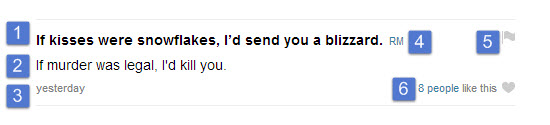
\includegraphics[width=0.85\textwidth]{Figures/Chapter4/sample_question.jpg}
	\caption[Sample question and answer]{Sample question and answer from ask.fm showing the question, the answer, when the question was answered, the user that asked the question, the report question flag and the number of likes that this question and answer has.}
	\label{fig:chapter4:sample_question}
\end{figure}

All questions and answers belonging to a single user can be displayed on a single web page. Initially, only the first 25 are displayed but a "View More" button makes it extremely easy to access all of a users questions and answers without the need for complicated scraping rules. Once all the questions and answers belonging to a user are displayed it is just a simple matter of saving the web page to a HTML file on disk.

Once the criteria to select potential users and the method to extract the users raw data was determined the final action was to download a suitably sized dataset. Having considered the downloading process in advance the goals were to obtain at least 100,000 questions and answers and to try and spread the distribution of the users as much as possible across the globe.  It was estimated that there would be an average of approximately 2,000 questions and answers per user account. To meet the first goal at least fifty accounts would be downloaded. To achieve the second goal the data was downloaded in three separate sessions each spaced over a twenty-four hour period. The first set was downloaded early in the morning local time at around 09:00. The second set was download in the early evening around 16:00. The final set was downloaded at 23:00 at night. The final action was to determine which users data to download. 

The stream page displays the most recently submitted questions and answers so this page was used to identify potential user accounts. Starting at the top, and working through all twenty five questions on the page, each users account was examined to determine if it met the criteria for selection. If it did then the users complete set of questions and answers were download. If the criteria were not met then the next users questions were examined until all questions on the stream had been reviewed. When there were no further users questions to be examined the stream was refreshed. The process was repeated until a proportional amount of user data had been downloaded at each time slot.

Upon completion, data from 57 accounts had been downloaded yielding 109,312 questions and answers. A cursory examination of the users showed that there was representation from North America, Australia / New Zealand and Europe.
\section{Initial Data Processing}
\label{section:initial_processing}

The next phase was to extract the individual elements from each question and answers combination. The questions and answers from 57 users were downloaded with each users data stored in a single HTML file. To extract the data from these files Python and the Beautiful Soup HTML parsing library were used. After extracting the data from each file, it was written to a table in a MySQL database. The entire process can be summarised as shown in Figure \ref{fig:chapter4:extract_data_from_html}.

\begin{figure}[htbp]
	\centering
	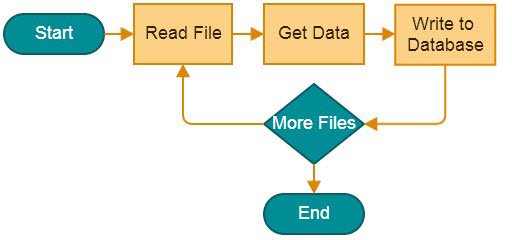
\includegraphics[width=0.5\textwidth]{Figures/Chapter4/extract_data_from_html.jpg}
	\caption[Simple process flow to extract data from HTML files]{Simple process flow to extract data from the HTML files downloaded from the Ask.fm website.}
	\label{fig:chapter4:extract_data_from_html}
\end{figure}

\subsection{Extract data from HTML Files}

Access to each HTML file is done using the glob and os packages. Each file is then parsed using the Beautiful Soup HTML parser (line 38). The script used to extract the data from the raw HTML files is included in Appendix \ref{app:parse_raw_data}. 

The individual data elements associated with each question and answer combination are contained within a HTML division element with a class attribute of \textit{``questionBox''}. A sample question box element is shown in Listing \ref{lst:chapter4.2:snipet_02}:

\begin{lstlisting}[language=html,caption={Sample question and answer HTML},label=lst:chapter4.2:snipet_02]
<div class='questionBox' id='question_box_107612243263'>
 <div class='question' dir='ltr'>
  <span>
   <span>I miss you</span>
  </span>
  <span class='author nowrap'>
   <a href='http://ask.fm/askerid'>
    askername
   </a>
  </span>
 </div>
 <div class='reportFlagBox '>
  <a href='http://ask.fm/userid/questions/107612243263'/>
 </div>
 <div class='answer' dir='ltr'>
  Text me?
 </div>
 <div class='time'>
  <a href='http://ask.fm/userid/answer/107612243263'>
   about 1 month ago
  </a>
 </div>
 <div class='likeList people-like-block'>
  <a href='http://ask.fm/likes/userid/question/107612243263' 
   1 person
  </a> likes this
 </div>
</div>
\end{lstlisting}

These data elements are examined in further detail later in this paper.

It is worth considering further the python in Appendix \ref{app:parse_raw_data} to understand how the data is extracted from the HTML files. As previously mentioned, each HTML file was parsed using the beautiful soup package resulting in an object called \verb|soup| that encapsulated all the file contents. From an earlier examination of the HTML it was known that each block of data was contained in a HTML division element that had a class attribute with a value of \verb|questionBox|. Line 55 shows how the \verb|soup.findAll()| method is applied to find all \verb|div| elements with a \verb|class| attribute with a value of \verb|questionBox| creating a list containing all question objects. Each question object is then individually retrieved for processing.

\begin{lstlisting}[firstnumber=55]
for a_question in soup.findAll("div", {"class": "questionBox"}):
\end{lstlisting}

Each of the seven data elements can then be extracted from this question object. Taking the question id first,  it is extracted from the \verb|id| attribute of the root question box division element. The value of the id attribute is split on the \verb|_| character and the question id is the third element of the array resulting from the split. In the sample HTML shown in Listing \ref{lst:chapter4.2:snipet_02} the question id is \verb|107612243263|. The python for this is shown on line 63. The \verb|strip| method simply removes any leading or trailing whitespace characters that may have been included in the extracted string.

\begin{lstlisting}[firstnumber=63]
question_id = a_question["id"].split("_")[2].strip()
\end{lstlisting}

The identification of the asker of the question and the number of likes that the question and answer have received are two more complicated examples because values for these elements may not exist so a check must be first performed to ascertain if the elements exist or not. To do this, a \verb|try| block is used. Taking the identification of the asker of the question as an example, the \verb|find| method is used on the question object to search for an element that has an \verb|author nowrap| attribute with a child \verb|a| element. If so then the asker identification is in contained in the \verb|href| attribute. As the value of this attribute is a URL the string is split on the \verb|/| character with the fourth value of the resulting array containing the required value. If the required elements do not exist in the question object, that is the question was asked anonymously, an exception is caught and the data element is set to an empty value:

\begin{lstlisting}[firstnumber=78]
try:
	if a_question.find(attrs="author nowrap").			\
	 	a["href"].split("/")[3]:
	  ask_id = a_question.find(attrs="author nowrap").	\
	  a["href"].split("/")[3].strip()
except (AttributeError, KeyError):
	ask_id = ""
\end{lstlisting}

The final step is to write the data extracted from the HTML files to a database. For this purpose a MySQL database called \verb|thesis| was created as well as a table called \verb|raw_data| to house the question and answer data elements. In the Python script the first step is to create a database connection and then using this connection create a cursor object. When the data elements for each question and answer block have been extracted the required SQL code is then executed to write the data to the database. All database related code is executed with a try block in case an exception is thrown. In Appendix \ref{app:parse_raw_data} lines 41 - 50 show where the database connection is created and lines 105 - 124 where each record extracted is written to the database. This is just a brief summary of some of the main functionality of the python script used. Other functionality not discussed includes making the users identification and the question number anonymous.

\subsection{Splitting the data}

The final part of the initial processing performed on the data was to split the 109,312 samples into three blocks of data. It was decided to divide the dataset into blocks of 10\% for initial classification, model training and test, 80\% to later simulate a stream of data arriving at the Ask.fm website and the final 10\% for validation purposes. The details of how the block of 80\% of the data and the second 10\% validation block will be explained later.

Before splitting the dataset, it was decided that the only criteria imposed would be that the proportions of questions per user should be maintained. For example, if user \verb|X| has 2,400 questions, after the split this user would have approximately 240 questions in the first block, 1,920 in the second block and 240 in the third. 

Although there are many ways to split data in the manner required, called stratified sampling, it was decided to use IBM SPSS Modeler. The model used is shown in Figure \ref{fig:chapter4:data_partitioning}.

\begin{figure}[htbp]
	\centering
	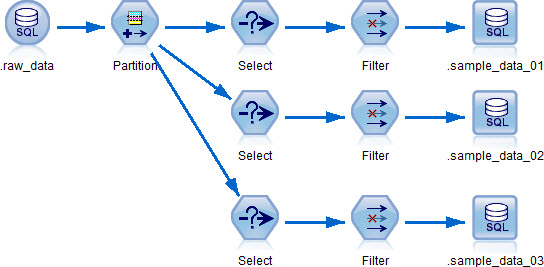
\includegraphics[width=0.75\textwidth]{Figures/Chapter4/data_partitioning.jpg}
	\caption[Partitioning data using IBM SPSS]{IBM SPSS Modeler process to split the dataset into three groups.}
	\label{fig:chapter4:data_partitioning}
\end{figure}

Using a \verb|SQL| operator a connection is created to the database and the raw data is extracted. It should be noted that this operator uses an ODBC connection to the database that must be created is advance. A \verb|Partition| operator is then used to split the data as required on the anonymous user id. The details of this operator are shown in Figure \ref{fig:chapter4:partition_operator}. The required split into three groups, based on the anonymous user identification field \verb|u_id| field, can be clearly seen. In the Figure \ref{fig:chapter4:partition_operator} it can also be seen that a new partition attribute is added to the data to help identify which group each record belongs to. This new attribute will be used in the next operator to split the data into the three required groups. 

\begin{figure}[htbp]
	\centering
	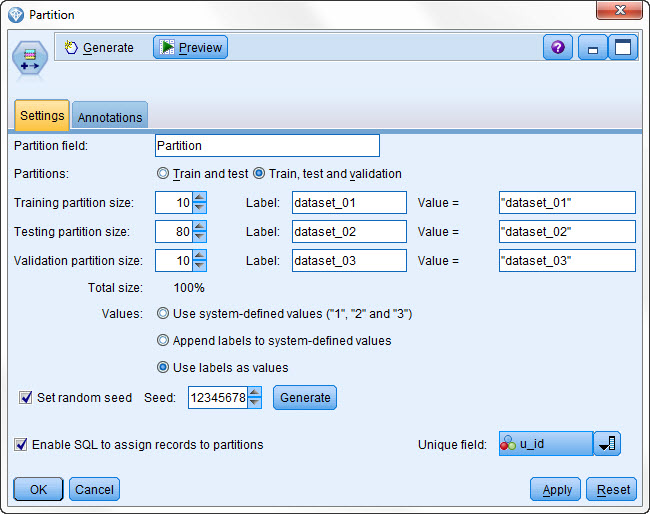
\includegraphics[width=0.75\textwidth]{Figures/Chapter4/partition_operator.jpg}
	\caption[Partition operator used generate a new attribute]{The Partition operator that is used generate a new partition attribute on which the data will be split.}
	\label{fig:chapter4:partition_operator}
\end{figure}

The output of the \verb|Partition| operator is then used as input into three separate \verb|Select| operators. The input to each of these operators is the same, the complete dataset, but as can be seen in Figure \ref{fig:chapter4:select_filter} only records that match the given condition, in this case \verb|Partition = "dataset_01"|, are passed through to the next operator which is the \verb|Filter| operator. Although it would be possible at this point to write the entire record of the question to the database, this would represent significant data repetition and redundancy. Using views in the database means that it is only necessary to write the anonymous question id of each record to the database. Once the question id is know then it will be possible to access any other attributes or columns as required using SQL. Only the anonymous question id, \verb|q_id|, is allowed pass through to the final operator where the anonymous question ids of the three blocks of data are each written to their respective tables created solely for this purpose.

\begin{figure}[htbp]
	\centering
	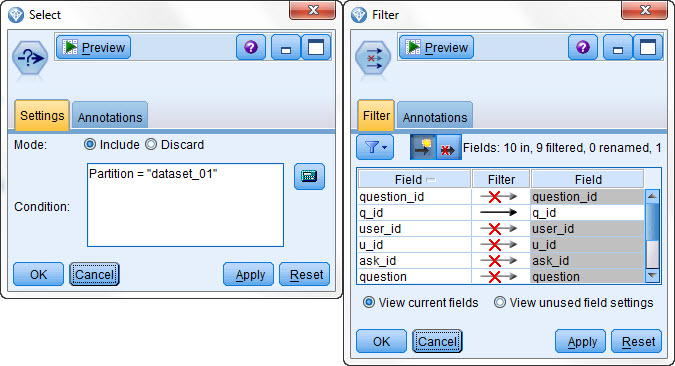
\includegraphics[width=0.75\textwidth]{Figures/Chapter4/select_filter.jpg}
	\caption[Select operator and the Filter operator settings]{The Select operator and the Filter operator settings.}
	\label{fig:chapter4:select_filter}
\end{figure}

Further details about the format, structure and contents of the data and the database housing the data at this point in the process is provided in the Section \ref{section:data_exploration}.


\section{Classification}
\label{section:data_classification}

The next task was to analyse the data selected for use in the development and training of a model and then classify each questions as either bullying or not bullying. As described in Chapter \ref{chapter3}, cyberbullying can take many forms such as flaming, outing, exclusion, flooding, cyberstalking, impersonation or masquerading, trolling and denigration of their victims. These attacks could then be categorised as sexual, racial, cultural or against the intelligence or physical appearance of a person or their socio-economic status to name but a few. The types and categories of cyberbullying are further examined and analysed to develop a sense of the criteria against which to evaluate each question. Once evaluated, each question will then be classified as bullying or not bullying.

\subsection{Cyberbullying Criteria}

This section provides more details about the type of on-line post, or in this case question, that should be considered as cyberbullying.

\textit{``Flaming''} is usually considered as off topic insults or attacks against an individual or group and are more typically seen in a bulletin board or discussion type forums. A classic example of flaming is where a discussion comparing the virtues of the Linux, Microsoft Windows and Apple Mac operating systems disintegrates into a series of posts where each side questions the intelligence of the other two groups for using such an obviously inferior product. In the context of the ask.fm dataset, it is unlikely that a series of posts of this type would be obviously detectable. The nature of the question and answer format, the order of the answers given, and their intermingling with other question would prevent it. Some questions that are obviously flaming made even be deleted or blocked. However, even if a series of questions that are flaming in their nature, either against an individual or a number of individuals, cannot be specifically identified as flaming their hostility, aggressiveness or derogatory sentiments would probably guarantee that they are identified as bullying. A user that purposefully starts, encourages or engages in such flaming activities is sometimes known as a \textit{``Troll''} and by denigrating or annoying people in this manner they are said to be \textit{``Trolling''}

The  term \textit{``outing''} is typically used to describe the disclosure of a persons sexual orientation, for example, revealing for the first time that a person is gay. As the users of the Ask.fm site are mostly teenagers and young adolescents, and because of the amount of sarcasm and black humour observed, it would be difficult reading isolated questions to determine whether a genuine outing has occurred. There is no facility to validate any such outing claim, or to determine if the question is just a slanderous attack. Regardless of these uncertainties, any post that appears to out someone or to question their sexual orientation must be considered as bullying.

Cyber \textit{``exclusion''} can be considered as any type of activity that purposefully excludes an individual or group from an event, a party, shopping trip or holiday, for example.  Alternatively, perhaps, they are prevented from joining a sports team or social group. This exclusion could take the form of inviting everyone to a party but then, explicitly, uninviting the excluded person in a public and humiliating manner. Another scenario could be to openly mock or taunt someone because they were prevented from joining a popular social clique in school. Any such obvious exclusionary activity seen in the Ask.fm dataset would be highlighted as bullying.

In some ways \textit{``flooding''} could be seen as similar in nature to a Denial of Service (DoS) attack on a website. A DoS attack is an attempt to interrupt the normal functioning of a website or make it unavailable to users by bombarding the site with so many requests that the sites response time to legitimate traffic is extremely slow or non-existent, rendering the site unusable. In a chat room, flooding could be seen as repeatedly, and in very quick succession, posting empty messages or the same message again and again to prevent other users in the chat room from voicing their opinion. Alternatively, in the context of the Ask.fm dataset, flooding could be considered as the repeated asking of the same question or requests for information. Such flooding activity, if seen, should be considered bullying. However, as the data has been both anonymised and randomised, or instances of flooding may already have been deleted by the targeted user, it may be difficult to identify.

Stalking is seen as the unwanted, obsessive and criminal intrusion into the personal life of an individual by another person. When computers or other electronic equipment is used it can be considered as \textit{``cyberstalking''}. The actions of a stalker can include activities such as a desire to control their victim, to subversively gather information about them, monitoring and anonymously commenting on their on-line activity and making claims of false victimisation against the target and  other false accusations such as defamation and libel. Other behaviours exhibited by the stalker may include flooding the victims with constant requests for personal information or for requests to meet in person. Any questions that are malicious in nature, from their content or tone, should be considered bullying. However, some questions, which may at first appear innocuous, for example ``how old are you'', ``where were you last night'' or ``send me a selfie'' should also be classified as bullying as they are requesting personal information which could be used by a potential stalker.

\textit{``Impersonation''} or \textit{``Masquerading''} is where a person creates a false identity, or assumes the identity of someone else, when posting or creating on-line content. Typically the reason for posting content using this assumed or false identity is to harm the reputation of the person they are pretending to be, by making what appear to be personally humiliating comments or by making harmful, harassing, confrontational or bullying remarks against another person. Alternatively the owner of a false account could  use it solely for the purpose of anonymously posting harmful content while observing on-line etiquette with their real name account. Due to the anonymous nature of the content on the Ask.fm site and the lack of any validation of a persons true identity it would be difficult if not impossible to ascertain whether a question is asked by a user masquerading or impersonating another person. However, it could also be argued that regardless of who posted the question if it meets any of the criteria that identify cyberbullying then it should be marked as such.

It is also important to consider the tone and content of a cyberbullying incident as well as the various forms that it may take. As well as threats of physical violence, the wishing of harm on a person, or by goading a perform to harm themselves, the tone of a cyberbullying attack can be categorised in many ways including gender, sexist, racial, cultural, nationality, ethnicity, colour or race, intellectual, appearance, religious or socio-economic. Questions that could be considered confrontational, libellous, defamatory or make unfounded accusations that are intended to be hurtful or that could result in unstated repercussions should be considered as bullying. 

Gender or sexist attacks would typically target women or sexual minorities, for example gay, lesbian, bisexual or transgender orientation. Simple examples of this type of cyberbullying would be name calling such as referring to a person as a \textit{``bitch''}, \textit{``faggot''} or \textit{``dyke''} or questions relating to sexual experience. Other more sinister types of these attacks would include unwanted sexual advances or invitations to engage in or descriptions of unsolicited sexual activity. An extreme case would be the threat or implication of rape. Racial or cultural bullying includes slurs or attacks against a cultural minority and its traditions, or direct attacks against a person based solely on their skin colour, ethnicity, race or nationality. Questions asking someone in a derogatory way if they are mentally or physically handicapped or questions that are hurtful or mean about their weight, height or general appearance are all bullying.

Though difficult to identify in isolation, text that may be considered grooming in nature should also be identified. There are multiple different categories of grooming approaches including Approach, Communicative Desensitisation, Compliment, Isolation and Reframing. Samples of each type of categories are \textit{``i just want to meet''}, \textit{``how cum''}, \textit{``you are a really cute girl''}, \textit{``are you alone''} and \textit{``let's have fun together''}  \cite{kontostathis_chatcoder:_2009}

It should be noted that profanity, without any of the other criteria listed here, would not, for the purposes of this research, be considered as cyberbullying.

The criteria for identifying cyberbullying can be summarised as follows:

\begin{enumerate}

	\item Can readily be identified as being attempts at flaming or of flooding.
	\item Is an obvious attempt to exclude or isolate an individual from a group or event.
	\item Could be perceived as stalking by overtly asking for personal information or photos 
	\item May be considered grooming where the question could be seen as an approach, an attempt to isolate or any of the other categories defined.
	\item Unnecessarily sexually explicit references or unsolicited invitations or by outing an individual whether real or perceived.
	\item Derogatory comments about race, culture, nationality, ethnicity or religion.

\end{enumerate}

\subsection{Dataset Classification}
Once the criteria to be used to identify a question as bullying had been determined the next step was to classify the block of questions that were to be used to train and test the initial model. Classification was a two step process. First all questions were reviewed and classified as either bullying, not bullying or discard. In total 10,914 question were reviewed. 1,644 were classified as bullying, 78 were classified as discard and the remainder as not bullying. Questions that were classified as discard contained only digits, emoticons or what appeared to be random characters. 

To validate that the classification criteria specified are both meaningful and understandable and that the original classification was repeatable, accurate and consistent, a random selection of 500 questions, 250 bullying and 250 not bullying, were independently classified by two other reviewers. Each reviewer was given the classification criteria described here and a print out of the original unedited questions. They were then asked to classify each sample question as either bullying or not bullying. The results from each reviewer is shown in Figure \ref{fig:chapter4:reviewer_results}

\begin{figure}[htbp]
	\centering
	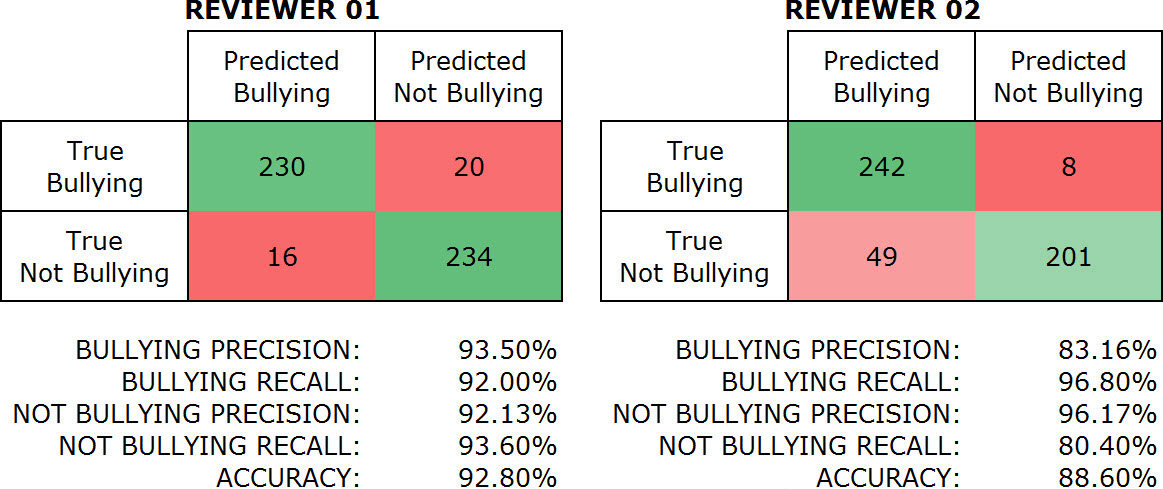
\includegraphics[width=0.9\textwidth]{Figures/Chapter4/reviewer_results.jpg}
	\caption[Independent classification review results]{Matrix showing the number of questions classified as bullying and as not bullying by two independent reviewers}
	\label{fig:chapter4:reviewer_results}
\end{figure}

In total, the first reviewer classified 246 questions as bullying of which 230 were originally identified as bullying. The second reviewer predicted 291 questions as bullying, of which 242 were originally identified as bullying. In total 224 of 250 sample questions, or just under 90\%, were identified by all three classifiers as bullying. However, 248 out of 250 sample bullying questions, or 99.2\%, were identified as bullying by two out of the three classifiers. Of note, 14 sample questions, that were originally classified as not bullying, were classified as bullying by both the independent reviewers. At just over 5.5\% this is not hugely significant but important to highlight. Overall, however, this was a very satisfactory validation of the both the classification criteria and the original classification of the complete dataset.

Before leaving this section, it is worth briefly examining some of the questions that were classified as bullying and understand why they were so classified. All the samples listed here are genuine examples from the Ask.fm dataset that was classified. Some of the samples have been abbreviated so as to highlight the relevant part of the question.

\begin{itemize}

	\item Asking someone their age. \\
	Asking how old they are could be very innocent and a genuine friendly request. However, it could just as easily be considered as stalking or as grooming. 
		\begin{itemize}
			\item \verb|Age?|
			\item \verb|How old are you?| 
		\end{itemize}
		
	\item Asking for information of an obviously private nature
		\begin{itemize}
			\item \verb|What Bra size are you?|
			\item \verb|can i have ur number?|
			\item \verb|How many ladies have you slept with?|
		\end{itemize} 

	\item Asking someone to post a picture or video of themselves often requesting specific parts of the body, clothes or naked.
		\begin{itemize}
			\item \verb|Puberty progress photo?|
			\item \verb|bikini picture?|
			\item \verb|Pap of you right now?|
		\end{itemize}

	\item Asking someone about their sexual experience or preferences
		\begin{itemize}
			\item \verb|Are you a virgin?|
			\item \verb|Are you good at giving head ?|
			\item \verb|butt or boobs|
		\end{itemize}
	
	\item Threatening physical violence or goading others to hurt themselves
		\begin{itemize}
			\item \dots \verb|Cut your self ugly saggy ass hoe|
			\item \dots \verb|I'm gonna beat your trashy little twig of an ass in so far| \\ \verb|     you'll puke it out| \dots
			\item \dots \verb|i will slap you across your f**king mouths|
		\end{itemize}

\end{itemize}

Before leaving this section it is important to note that these are only a small example of the questions that were classified as bullying. The content of a large proportion of the question would be considered crude, vulgar and too offensive to list here.
\section{Data Exploration}
\label{section:data_exploration}

At this point the data from the ask.fm site has been analysed, extracted and classified. The next step is to explore the data and get a better understanding of its contents and quality. It could be argued that an exploration of the data would have been better performed before it was classified. However, because of the simplicity of the structure of the data used in this research project it was decided that there was nothing to be gained in performing the exploration first. In this section, the structure of the data is briefly described before giving details of the exploration performed and also the finding. Finally the quality of the data is reviewed.

\subsection{Data Description}
In the previous section the classification process was described where each question was classified as bullying, not bullying or discard. This classification attribute, along with the anonymous question identify was imported back into the MySQL database to allow further exploration of the data and for future access. A simple view of the database schema is shown in Figure \ref{fig:chapter4:thesis_schema}. This is the view of the schema automatically generated by the MySQL Workbench Tool.

\begin{figure}[htbp]
	\centering
	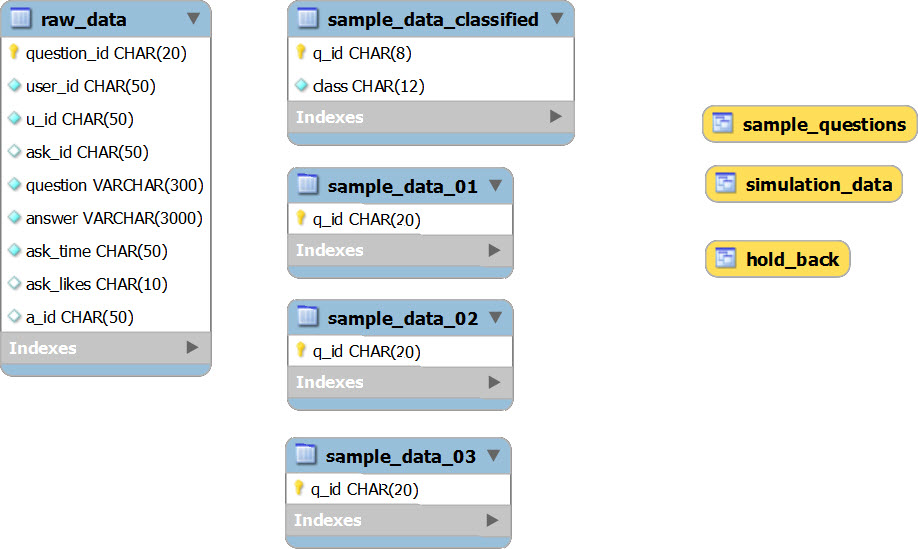
\includegraphics[width=0.85\textwidth]{Figures/Chapter4/thesis_schema.jpg}
	\caption[View of the thesis schema]{A simple representation of the thesis schema.}
	\label{fig:chapter4:thesis_schema}
\end{figure}

To recap, the \verb|raw_data| table is the all of data as extracted from the HTML files of each of users whose questions were scraped earlier. The \verb|sample_data_01| table contains the anonymous question ids, representing 10\% of all questions, to be used for generation of the model and the \verb|sample_data_classified| table is the same list of the anonymous question ids and their classification label. From these tables the \verb|sample_questions| view was created to allow easy access to the primary data attributes. Over the course of the data exploration exercise many views of the data were created. Table \ref{tab:chapter4:rawdata} provides a brief description of each of the attributes in the \verb|raw_data| table. The only other attribute shown that is not included in this table is the \verb|class| attribute which holds the classification of whether the question is bullying or not bullying.

\begin{table}[h]
\centering
\caption[Description of raw\_data table]{Table describing the purpose of each attribute in the raw\_data table.}
\label{tab:chapter4:rawdata}
\begin{tabular}{ll}
	\toprule
    \textbf{Attribute}    & \textbf{Description}                   \\
    \midrule
    question\_id & The ask.fm question id        \\
    q\_id        & The anonymous question id     \\
    user\_id     & The ask.fm id of the user     \\
    u\_id        & The anonymous id of the user  \\
    ask\_id      & The ask.fm id of the asker    \\
    a\_id        & The anonymous id of the asker \\
    question     & The question                  \\
    answer       & The answer                    \\
    ask\_time    & When the question was asked   \\
    ask\_likes   & The number of likes received  \\
    \bottomrule
    \end{tabular}
\end{table}

\subsection{Data Quality}
Upon review of the data in the \verb|raw_data| table, it was immediately apparent that there were some minor issues with the text in the question and answers field. As initially only the questions would be used this was where effort was concentrated when determining data quality.

\begin{itemize}

	\item Questions with only images as answers appeared empty \\
	These are of no use in the automated classification of the question. There is no feasible way to replace a picture with text so these records will be removed from the dataset.
	\item Records with only numerical answers \\
	These will be of little value when trying to establish what features help identify text as bullying so will also be removed. 
	\item Records where part or all of the text was not English. \\
	Every effort was made though to only select English speaking users. There was little evidence of questions in languages other than English so no further investigation or processing is required.
	\item Records where non ASCII characters were used \\
	There was some evidence of the use of non ASCII characters. To simplify and standardise word tokens non ASCII characters will either be removed or replaced with their ASCII equivalent.
	\item Slang words, emoticons and abbreviations \\
	Slang words are usually very descriptive in nature and will be useful when developing the classification model. There is no need to attempt to identify, remove or replace these words. Emoticons are typically inconsistently used and often the same emoticon sentiment can be characterised in many different ways. Emoticons will be removed. To preserve sentence integrity, abbreviations should be replaced with the correct word token.
	\item Repeated characters \\
	Sometimes certain letters in words are repeated to emphasise the word. Where appropriate these repeated letters should be removed to reduce the number of distinct word tokens in the corpus.
	
\end{itemize}

These issues will further investigated and handled in Section \ref{section:data_prepatation}.

\subsection{Data Exploration}

Now that there is a basic understanding of the data it will be explored in more detail by visualising some of the key attributes. There is not actually much exploration required as the dataset is so simple. The first aspect to be examined is the number of records, questions, each user contributed to the total dataset and to ensure that when this total number of records was partitioned into the three separate data blocks that the approximate user to question ratios were maintained. It is also important to ensure that an average of 10\% of each users records were allocated to the block of data to be used for modelling. The total number of records per user is shown in the top chart in Figure \ref{fig:chapter4:user_distributions}. The criteria for user selection was that each user should have answered at least 1,000 question and no more than approximately 4,000. As can be seen there is a good distribution of the numbers of questions and, although the top three number of questions answered are greater than 4000, it can be said that this criterion has been met. The middle and bottom charts show the count of records each user contributed to the training dataset and the percentage of their total number of questions that this represents respectively. Although it can be seen that the percentages, at the extremes, vary between approximately 8.3\% and 11.7\%, at an overall average value of 9.92\% and a standard deviation of 0.7\% this distribution is acceptable.

\begin{figure}[htbp]
	\centering
	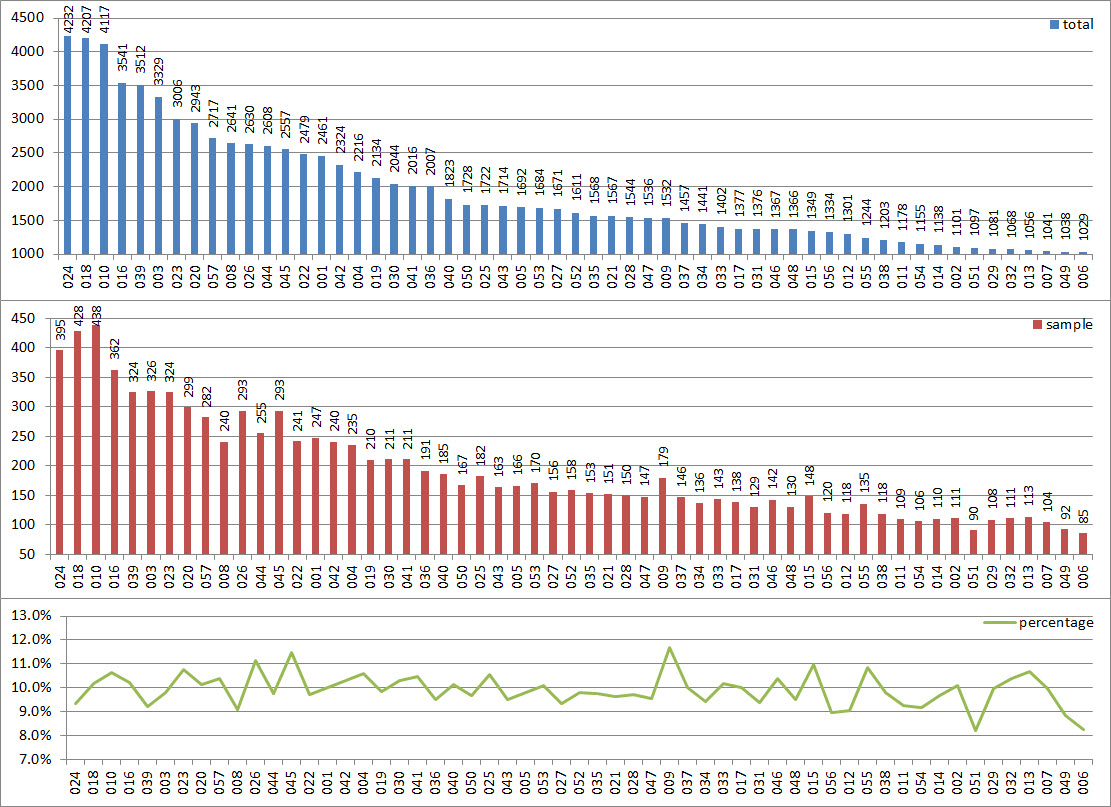
\includegraphics[width=1\textwidth]{Figures/Chapter4/user_distributions.jpg}
	\caption[Distribution of user records]{Distribution of users records showing the total number per user and the number and percentage of each users records in the training dataset}
	\label{fig:chapter4:user_distributions}
\end{figure}

Next the sample questions that will be used for modelling are further explored. The first two attributes to be examined are the distribution of the questions, between the bullying and not bullying classes, and an analysis of the number of anonymous questions that are asked. As shown in Figure \ref{fig:chapter4:class_distribution} approximately 1 question in every 7 was classified as bullying and that slightly less than 1\% of all question were identified as being not suitable for inclusion and could be discarded. The ratio of bullying question to not bullying questions is in line with figures obtained from other research projects in this area. In total 1,644 questions were classified as bullying.

\begin{figure}[htbp]
	\centering
	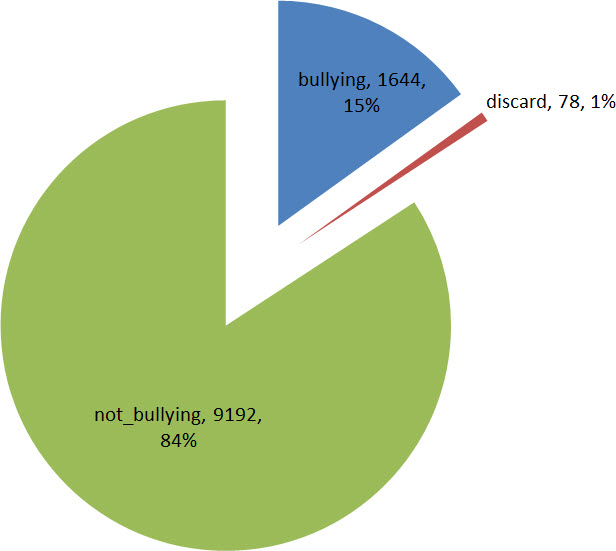
\includegraphics[width=0.55\textwidth]{Figures/Chapter4/class_distribution.jpg}
	\caption[Class Distribution of Sample Questions]{Class Distribution of Sample Questions}
	\label{fig:chapter4:class_distribution}
\end{figure}

\begin{figure}[htbp]
	\centering
	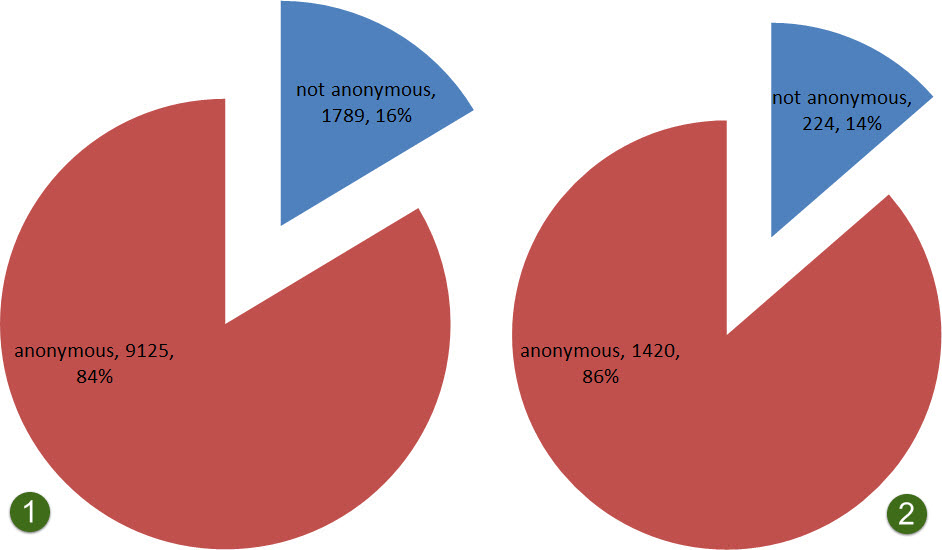
\includegraphics[width=0.8\textwidth]{Figures/Chapter4/anonymous_distribution.jpg}
	\caption[Sample Questions asked Anonymously]{Ratio of all questions asked anonymously (1) and ratio of questions classified as bullying asked anonymously (2)}
	\label{fig:chapter4:anonymous_distribution}
\end{figure}

The number of questions that were asked anonymously, and also the number of questions classified as bullying that were asked anonymously was also examined. There are 10,914 records in the sample questions dataset and it was noticed immediately that the percentage of anonymous questions that are asked was extremely high at 84\%. Unsurprisingly the number of anonymous questions that were classified as bullying was also very high at 86\% as shown on the right hand side of Figure \ref{fig:chapter4:anonymous_distribution}. Of the 1,644 questions that were classified as bullying 1,420 were asked anonymously and 224 were not asked anonymously.

Table \ref{tab:chapter4:not_anon_bullying} takes a closer look at the 224 question that were not asked anonymously. Two-thirds of the questions that were not asked anonymously were single questions asked by a user. Including instances where an identifiable user asked two questions that were classified as bullying, nearly 91\% of all bullying questions that were not asked anonymously were asked by a user who only asked one or two bullying questions. In total 5 users asked three or more anonymous bullying questions. In each case the bullying questions were asked to the same user. For example, the user identified by id \verb|4145| asked user \verb|57| seven questions, out of a total of thirty seven, that were classified as bullying. This suggests a familiarity between the two users and perhaps the questions are not bullying but just banter between two friends. However, as the total number of questions in this category are low, and the primary goal of this research is solely the identification of bullying posts, such considerations are not in scope now but could possibly be included in any future work.

\begin{table}[h]
\centering
\caption[Bullying questions that are not anonymous]{Table showing the break down of questions that were not asked anonymously by the id of the asker.}
\label{tab:chapter4:not_anon_bullying}
\begin{tabular}{rrrc}
	\toprule
    \textbf{Questions Asked} & \textbf{\# Users} & \textbf{\# Questions} & \textbf{Percentage}            \\
    \midrule
	7	& 1		&	7	&	3.1\%	\\
	4	& 2		&	8	&	3.6\%	\\
	3	& 2		&	6	&	2.7\%	\\
	2	& 27	&	54	&	24.1\%	\\
	1	& 149	&	149	&	66.5\%	\\
    \bottomrule
    \end{tabular}
\end{table}

The average length of questions classified as bullying and those classified as not bullying was analysed. As shown in Figure \ref{fig:chapter4:avg_question_len} the average length of a question that was classified as bullying is nearly 19\% longer than a question that is not. However with an overall average length of 42.3 with a standard deviation of 42.2 this difference in question lengths does not appear to be of great importance.

\begin{figure}[htbp]
	\centering
	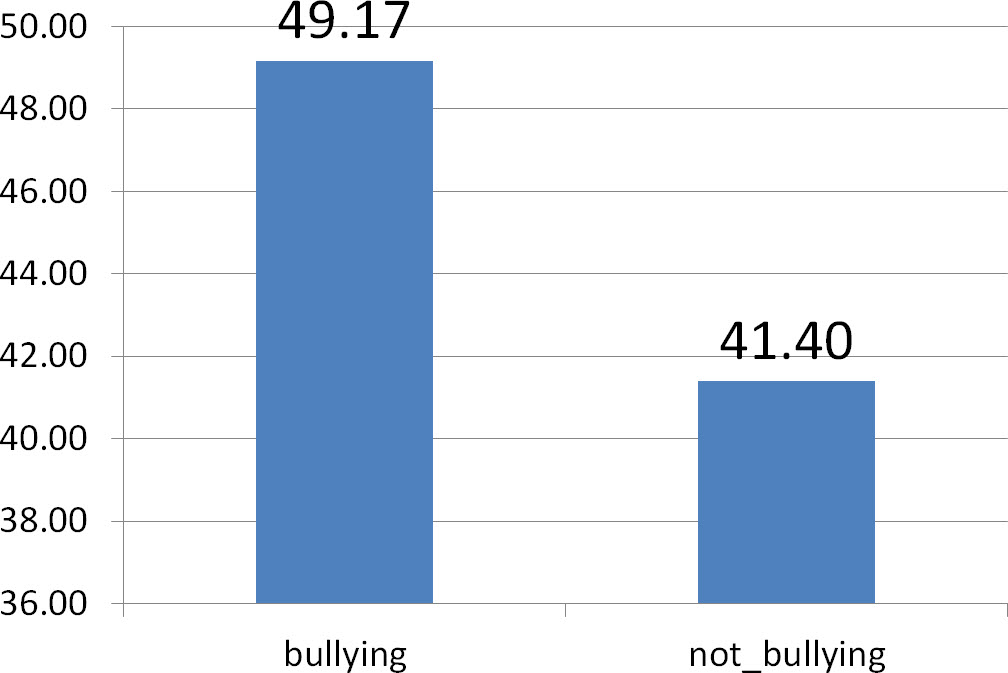
\includegraphics[width=0.5\textwidth]{Figures/Chapter4/avg_question_len.jpg}
	\caption[Average question length per class]{The average question length for questions classed as bullying and those that are not.}
	\label{fig:chapter4:avg_question_len}
\end{figure}

The corpus of distinct words, and the count of the number of times each word was used, was then examined. A simple Python script was developed to identify all distinct words in the corpus and also count the number of occurrences of each word. Unique words, or tokens, that were at least 2 characters long were considered. There were 12,162 distinct string tokens that met this criterion with 85988 tokens in total. The average word occurrence frequency was 7.07 but with a massive standard deviation of 69.38. The questions were then divided into not bullying and bullying corpora, and the analysis performed again. Table \ref{tab:chapter4:word_count} shows the twenty most frequently occurring words for all questions, not bullying questions and bullying questions. A quick glance at the table shows that when these words are considered there is no obvious discernible difference between the words in the not bullying questions corpus and the words in the bullying questions corpus. When comparing the top twenty words in the not bullying and bullying classes it can be seen that four in every five words, or 80\%, appear in both lists.

\begin{table}[h]
\centering
\caption[Distinct word counts]{Table showing distinct word counts for all questions and separately for not bullying and bullying questions}
\label{tab:chapter4:word_count}
\begin{tabular}{lrlrlr}
	\toprule
	\multicolumn{2}{c}{\textbf{Total}} & \multicolumn{2}{c}{\textbf{Not Bullying}} & \multicolumn{2}{c}{\textbf{Bullying}}\\
	\cmidrule(r){1-2}
	\cmidrule(r){3-4}
	\cmidrule(r){5-6}
    \textbf{Word} & \textbf{Count} & \textbf{Word} & \textbf{Count} & \textbf{Word} & \textbf{Count}           \\
    \midrule
	you		& 5399	&	you		&	4492	&	you		&	907	\\
	your	& 1759	&	what	&	1520	&	your	&	370	\\
	the		& 1716	&	the		&	1488	&	and		&	313	\\
	to		& 1701	&	do		&	1422	&	to		&	283	\\
	what	& 1657	&	to		&	1418	&	the		&	228	\\
	do		& 1573	&	your	&	1389	&	are		&	223	\\
	and		& 1345	&	and		&	1032	&	of		&	172	\\
	is		& 1114	&	is		&	986		&	have	&	158	\\
	are		& 1076	&	are		&	853		&	do		&	151	\\
	like	& 895	&	like	&	753		&	like	&	142	\\
	in		& 816	&	in		&	687		&	so		&	137	\\
	of		& 772	&	on		&	612		&	what	&	137	\\
	have	& 726	&	of		&	600		&	in		&	129	\\
	on		& 714	&	would	&	571		&	is		&	128	\\
	would	& 650	&	have	&	568		&	with	&	127	\\
	so		& 632	&	that	&	517		&	me		&	126	\\
	that	& 610	&	if		&	497		&	on		&	102	\\
	it		& 569	&	so		&	495		&	ur		&	102	\\
	now		& 561	&	who		&	489		&	how		&	97	\\
	who		& 555	&	how		&	464		&	that	&	93	\\
    \bottomrule
    \end{tabular}
\end{table}

This word count exploration was performed again. In addition to only selecting words that were at least 2 characters long, all English stop words defined in the Python Natural Language Tool Kit were removed. Now, whilst there are still 12,044 distinct tokens, overall there are only 49,942 token instances, a 42\% decrease, with an average word occurrence of only 4.15. The results of this word count analysis is shown in Table \ref{tab:chapter4:word_count_nostop}.  Although there is now some better differentiation between the not bullying and bullying questions, there are still 12 common words in the top twenty words of each category. This suggests that building a model to predict the class of questions using word counts alone will not be predictive enough and that maybe additional strategies will need to be considered.

\begin{table}[h]
\centering
\caption[Distinct word counts, no stop words]{Table showing distinct word counts for all questions and separately for not bullying and bullying questions with stop words removed}
\label{tab:chapter4:word_count_nostop}
\begin{tabular}{lrlrlr}
	\toprule
	\multicolumn{2}{c}{\textbf{Total}} & \multicolumn{2}{c}{\textbf{Not Bullying}} & \multicolumn{2}{c}{\textbf{Bullying}}\\
	\cmidrule(r){1-2}
	\cmidrule(r){3-4}
	\cmidrule(r){5-6}
    \textbf{Word} & \textbf{Count} & \textbf{Word} & \textbf{Count} & \textbf{Word} & \textbf{Count}           \\
    \midrule
	like	& 895	&	like	&	753	&	like	&	142	\\
	would	& 650	&	would	&	571	&	ur		&	102	\\
	don't	& 349	&	think	&	307	&	would	&	79	\\
	think	& 344	&	don't	&	276	&	don't	&	73	\\
	know	& 327	&	know	&	260	&	pic		&	69	\\
	ur		& 323	&	love	&	258	&	know	&	67	\\
	love	& 302	&	:)		&	252	&	get		&	58	\\
	:)		& 294	&	favorite&	245	&	post	&	56	\\
	you're	& 292	&	you're	&	238	&	f**k	&	56	\\
	get		& 285	&	get		&	227	&	you're	&	54	\\
	really	& 261	&	best	&	222	&	want	&	53	\\
	one		& 253	&	ur		&	221	&	i'm		&	52	\\
	favourite& 250	&	one		&	220	&	really	&	50	\\
	i'm		& 238	&	people	&	213	&	see		&	50	\\
	best	& 238	&	really	&	211	&	go		&	50	\\
	go		& 238	&	what's	&	208	&	love	&	44	\\
	people	& 235	&	ever	&	194	&	old		&	42	\\
	ever	& 233	&	thing	&	189	&	bitch	&	42	\\
	what's	& 226	&	go		&	188	&	right	&	40	\\
	want	& 224	&	i'm		&	186	&	ever	&	39	\\
    \bottomrule
    \end{tabular}
\end{table}

A common strategy used in text mining classification is the generation of term n-grams. N-grams have the effect of concatenating together two or more tokens to form new hopefully more predictive tokens. For example the quote \textit{``to be or not to be''} produces the following tri-grams:

\begin{itemize}

	\item to\_be\_or
	\item be\_or\_not
	\item or\_not\_to
	\item not\_to\_be
	
\end{itemize}

Bi-grams, two tokens, and tri-grams, three tokens, word lists were generated from the bullying and not bullying questions examined earlier. As before only words or tokens that were at least two characters long were considered. Word or token frequencies were determined and these results are shown in Tables \ref{tab:chapter4:word_count_bi-gram} and \ref{tab:chapter4:word_count_tri-gram}.

\begin{table}[h]
\centering
\caption[Distinct bi-gram word counts]{Table showing distinct counts of bi-gram tokens for not bullying and bullying questions with and without stop words}
\label{tab:chapter4:word_count_bi-gram}
\begin{tabular}{lrlrlrlr}
	\toprule
	\multicolumn{4}{c}{\textbf{Not Bullying}} & \multicolumn{4}{c}{\textbf{Bullying}} \\
	\cmidrule(r){1-4}
	\cmidrule(r){5-8}
	\multicolumn{2}{c}{\textbf{With Stopwords}} & \multicolumn{2}{c}{\textbf{No Stopwords}} & \multicolumn{2}{c}{\textbf{With Stopwords}} & \multicolumn{2}{c}{\textbf{No Stopwords}} \\
    \midrule
	do\_you			& 959 &	would\_like		 & 74 &	are\_you  &	93 & right\_now		& 28	\\
	what\_is		& 344 &	would\_be		 & 47 &	do\_you   &	72 & wearing\_right	& 20	\\
	are\_you		& 342 &	don't\_know		 & 42 &	you\_have &	42 & post\_pic		& 16	\\
	would\_you		& 318 &	one\_thing		 & 41 &	you\_are  &	40 & don't\_know	& 15	\\
	if\_you			& 259 &	last\_time		 & 40 &	what\_are &	40 & old\_you		& 14	\\
	you\_like		& 246 &	what's\_favorite & 40 &	how\_old  &	37 & cut\_cut		& 8	\\
	is\_the			& 215 &	last\_person	 & 33 &	want\_to  &	31 & post\_picture	& 7	\\
	is\_your		& 198 &	right\_now		 & 32 &	if\_you   &	30 & would\_go		& 6	\\
	your\_favorite	& 184 &	best\_friends	 & 27 &	of\_you   &	30 & dont\_like		& 6	\\
	have\_you		& 179 &	best\_friend	 & 25 &	pic\_of   &	29 & look\_like		& 6	\\
    \bottomrule
    \end{tabular}
\end{table}

Examining the top ten most frequently occurring bi-gram tokens some features are immediately apparent. The first most obvious thing to notice is that where stop words are not removed only three out of the ten not bullying tokens, 30\%, also appear in the bullying list. When compared to the top ten uni-grams, single words tokens, where 80\% of the top ten tokens appears in both lists this represents a possible indicator that bi-grams would be of more use in the classification of unseen questions. When stop words are removed the number of common words fell from six out of ten repeated uni-grams, 60\%, to only two out of 10 or 20\% bi-grams. Also of note is the use of \verb|you|, the second person pronoun. When stop words are not removed \verb|you| is prominent, appearing in six out of the top ten bi-grams in both the not bullying and word bullying lists. Another pronoun, \verb|your|, also appears twice in the not bullying top ten list. However, when stop words are removed \verb|you| does not appear at all in the not bullying top ten and only once in the bullying top ten. This observation flies somewhat in the face of \citet{yin_detection_2009} which mentioned that when reviewing their dataset it was noticed that a lot of the posts classified as harassment contained foul language used in conjunction with pronouns, particularly second person personal pronouns such as ``you'', ``your'' and ``yourself''. An examination of the data from Ask.fm does not, at first sight, corroborate these findings. 

\begin{table}[h]
\centering
\caption[Distinct tri-gram word counts]{Table showing distinct counts of tri-gram tokens for not bullying and bullying questions with and without stop words}
\label{tab:chapter4:word_count_tri-gram}
\begin{tabular}{lrlr}
	\toprule
	\multicolumn{4}{c}{\textbf{Not Bullying}} \\
	\cmidrule(r){1-4}
	\multicolumn{2}{c}{\textbf{With Stopwords}} & \multicolumn{2}{c}{\textbf{No Stopwords}} \\
    \midrule
	what\_is\_your		& 154 &	would\_like\_meet		& 74 \\
	what\_do\_you		& 153 &	people\_think\_you		& 47 \\
	do\_you\_think		& 133 &	favorite\_month\_year	& 42 \\
	what\_is\_the		& 132 &	many\_times\_day		& 41 \\
	do\_you\_like		& 128 &	gift\_would\_like		& 40 \\
	is\_your\_favorite	& 110 &	think\_people\_think	& 40 \\
	if\_you\_could		& 94 &	what's\_longest\_you've	& 33 \\
	what\_would\_you	& 86 &	last\_thing\_made		& 32 \\
	was\_the\_last		& 79 &	anyone\_right\_now		& 27 \\
	you\_like\_to		& 76 &	made\_happy\_today		& 25 \\
    \bottomrule
    \end{tabular}
\begin{tabular}{lrlr}
	\toprule
	\multicolumn{4}{c}{\textbf{Bullying}} \\
	\cmidrule(r){1-4}
	\multicolumn{2}{c}{\textbf{With Stopwords}} & \multicolumn{2}{c}{\textbf{No Stopwords}} \\
    \midrule
	what\_are\_you		& 30 &	wearing\_right\_now		& 20 \\
	how\_old\_are		& 24 &	cut\_cut\_cut			& 7 \\
	are\_you\_wearing	& 21 &	last\_person\_kissed?	& 5 \\
	wearing\_right\_now	& 20 &	whoever\_likes\_thinks	& 4 \\
	you\_wearing\_right	& 20 &	see\_window\_post		& 4 \\
	old\_are\_you		& 13 &	window\_post\_pic		& 4 \\
	have\_you\_ever		& 11 &	slept\_ex\_bf			& 3 \\
	of\_you\_and		& 10 &	shannon\_slept\_ex		& 3 \\
	post\_pic\_of		& 10 &	likes\_thinks\_you're	& 3 \\
	do\_you\_have		& 9  &	ex\_bf\_max				& 3 \\
    \bottomrule
    \end{tabular}
\end{table}

An examination of the tri-gram tokens in all categories showed that the top ten most frequently occurring tokens were all unique. Expanding this type of comparison to the top fifty tokens, it was found that when stop words were included three out of every ten tokens, or 30\%, appeared on both the bullying and not bullying lists. Expanding this to the top 100 tokens the repetition fell further to between 24\% and 20\% respectively. Examining next the tri-gram tokens where the stop words had been removed was even more revealing. Only two of the top one hundred not bullying tokens appeared anywhere in the bullying list. In the other direction none of the top 67 bullying tokens appeared anywhere in the top one hundred not bullying tokens. The reason the top 67 bullying tokens were chosen is because after these all tokens only had a frequency of one. Expanding the search to include all not bullying and bullying tri-grams, where the stop words had been removed, showed that only 57 tokens appeared in both lists. This represents 57 out of 21031 not bullying tri-grams, approximately 0.27\%, and 57 out of 5858 bullying tri-grams or 0.97\%. This finding would further support the suggestion that tri-gram tokens should prove to be very good predictors when it comes to developing the models.

One final set of measurements worth considering is the count of distinct tokens in each word list generated and also the average number of times each occurred. This data is summarised in Table \ref{tab:chapter4:word_distribution}. The data is divided into three sections. The first section describes the dataset when all the tokens are considered together. The second describes the not bullying data and the third the bullying data. As previously mentioned there were 12,162 unique uni-grams with 10,514 occurring in the not bullying dataset and 3,598 occurring in the bullying dataset. Delving a little deeper into this information it was discovered that of the 10,514 not bullying tokens 8,238 of these only occurred in the not bullying set showing that over 78\% of these tokens would be good predictors of a not bullying question. Taking the 3,598 bullying token it was seen that 1,575 of these tokens, or approximately 44\%, only occurred in the bullying list. Taking bi-gram tokens next, the percentages of distinct tokens used in either the not bullying dataset or the bullying data set rise to 97\% and 73\% respectively. This diverging of the common words between the two datasets continues all the way up to the tri-gram tokens with stop words removed where, as previously seen, over 99\% of the tokens in each dataset are unique. 

\begin{table}[h]
\centering
\caption[Unique tokens, total count and average frequency]{Table showing the number of distinct tokens in each dataset as well as the total token counts and average frequencies}
\label{tab:chapter4:word_distribution}
\begin{tabular}{lrrr}
	\toprule
	{\textbf{Token}} 		& {\textbf{Unique}} & {\textbf{Total}} & {\textbf{Average}}  \\
	{\textbf{description}}	& {\textbf{Tokens}} & {\textbf{Count}} & {\textbf{Frequency}}  \\
    \midrule
    \midrule
    \multicolumn{1}{l}{\textbf{All Words}} \\
	\cmidrule(l){1-1}
	Uni-Grams					& 12162 &	85988	& 7.1 \\
	Bi-Grams					& 41012 &	75128	& 1.8 \\
	Tri-Grams					& 51111 &	64983	& 1.3 \\
	Uni-Grams No Stop Words		& 12044 &	49942	& 4.1 \\
	Bi-Grams No Stop Words		& 31370 &	39125	& 1.2 \\
	Tri-Grams No Stop Words		& 27106 &	29567	& 1.1 \\
    \midrule 
    \midrule
    \multicolumn{1}{l}{\textbf{Not Bullying}} \\
	\cmidrule(l){1-1}
	Uni-Grams					& 10514 &	70722	& 6.7 \\
	Bi-Grams					& 33665 &	61557	& 1.8 \\
	Tri-Grams					& 40913 &	52981	& 1.3 \\
	Uni-Grams No Stop Words		& 10397 &	40831	& 3.9 \\
	Bi-Grams No Stop Words		& 25204 &	31706	& 1.3 \\
	Tri-Grams No Stop Words		& 21391 &	23604	& 1.1 \\
    \midrule
    \midrule 
    \multicolumn{1}{l}{\textbf{Bullying}} \\
	\cmidrule(l){1-1}
	Uni-Grams					& 3598 &	15208	& 4.2 \\
	Bi-Grams					& 9979 &	13565	& 1.4 \\
	Tri-Grams					& 11086 &	11998	& 1.1 \\
	Uni-grams No Stop Words		& 3489 &	9053	& 2.6 \\
	Bi-Grams No Stop Words		& 6847 &	7413	& 1.1 \\
	Tri-Grams No Stop Words		& 5858 &	5959	& 1.0 \\
    \bottomrule
    \end{tabular}
\end{table}

Next, the distribution of the tokens is further examined and visualised but from Table \ref{tab:chapter4:word_distribution} it is clear to see that the average frequency of each token falls from 7.1 for all uni-grams tokens to 4.1 for uni-grams where stop words have been removed all the way down to nearly a 1:1 ratio for bullying tri-grams where stop words are removed. This shows that very few tokens appear more than once in this tri-gram dataset. This observation suggests that a model based solely on these tri-gram tokens may, in fact, be over trained and would not generalise well to unseen data. This contradicts the earlier suggestion that tri-grams would be good predictors and must be taken into consideration and examined when models are being developed.

\subsection{Data Visualisation}
To visual the not bullying and bullying classes, word clouds, generated using the IBM Many Eyes tool, were used. Uni-grams were considered first and the results of these word clouds can be seen in Figures \ref{fig:chapter4:not_bullying_wordcloud},  \ref{fig:chapter4:bullying_wordcloud}.  When generating the visualisations only the fifty most frequently occurring words were used. It is very clearly seen that \verb|you| dominates both word clouds.


\begin{figure}[!htb]
	\centering
	
\includegraphics[width=0.8\textwidth]{Figures/Chapter4/not_bullying_wordcloud.jpg}
	\caption[Word cloud of not bullying words]{Word cloud of the 50 most frequently occurring words in questions classified as not bullying}
	\label{fig:chapter4:not_bullying_wordcloud}
\end{figure}

\begin{figure}[!htb]
	\centering
	
\includegraphics[width=0.8\textwidth]{Figures/Chapter4/bullying_wordcloud.jpg}
	\caption[Word cloud of bullying words]{Word cloud of the 50 most frequently occurring words in questions classified as bullying}
	\label{fig:chapter4:bullying_wordcloud}
\end{figure}

The exercise was then repeated with the uni-gram tokens where the NLTK stop words had been removed. The two word lists were loaded onto the Many Eyes website and visualised using the same settings as before. Figures  \ref{fig:chapter4:not_bullying_wordcloud_filtered} and \ref{fig:chapter4:bullying_wordcloud_filtered} show the results. It is immediately obvious that the words maps now appear more balanced with a better distribution of word weights across the images. Even so some words, for example \verb|like|, \verb|would|, \verb|don't| and \verb|know|, are still prominent in both classes. It was also observed that some stop words, for example \verb|you|, were still appearing in the word clouds when the token should have been removed. After some investigation it was discovered that the NLTK did not removed stop words where there was an adjacent punctuation character, for example \verb|you!|. These punctuation characters appear to have been striped when the data was loaded into Many Eyes explaining why they are still seen.  

\begin{figure}[!htb]
	\centering
	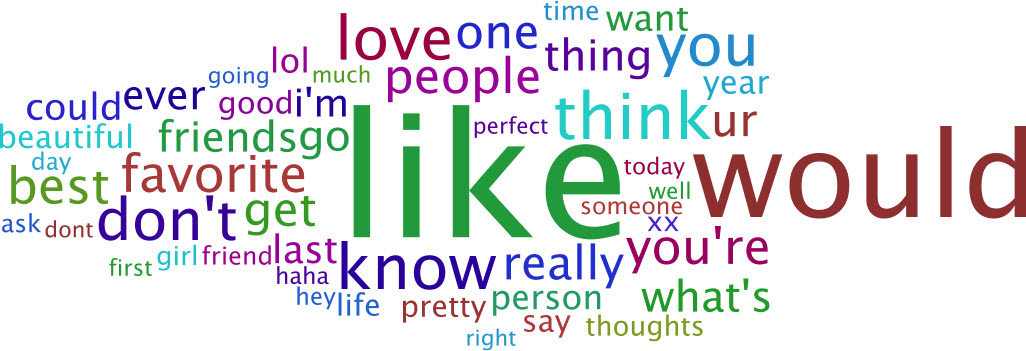
\includegraphics[width=0.8\textwidth]{Figures/Chapter4/not_bullying_wordcloud_filtered.jpg}
	\caption[Filtered word cloud of not bullying words]{Filtered word cloud of the 50 most frequently occurring words in questions classified as not bullying with stop words filtered out}
	\label{fig:chapter4:not_bullying_wordcloud_filtered}
\end{figure}

\begin{figure}[!htb]
	\centering
	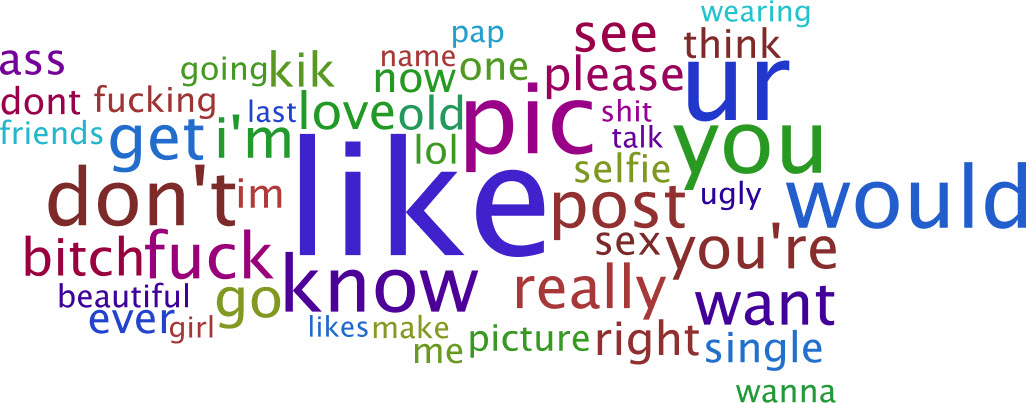
\includegraphics[width=0.8\textwidth]{Figures/Chapter4/bullying_wordcloud_filtered.jpg}
	\caption[Filtered word cloud of bullying words]{Filtered word cloud of the 50 most frequently occurring words in questions classified as bullying with stop words filtered out}
	\label{fig:chapter4:bullying_wordcloud_filtered}
\end{figure}

Whilst the word clouds present a nice way of visualising the frequencies of words in each of the categories, to generate a cloud for all the permutations already highlighted would be very time consuming. Also, any analysis performed on them would be subjective. For example, in Figure \ref{fig:chapter4:bullying_wordcloud_filtered} which word is more prominent \verb|ur| or \verb|pick|. A better way to visualise how the frequencies of words, or tokens, are distributed across each dataset is shown in Figure \ref{fig:chapter4:word_frequencies}. These three graphs shown the normalised word frequencies distributions for the 250 most frequently tokens for all tokens, labelled (1) in the diagram, all not bullying tokens, labelled (2) and all bullying tokens. For brevity, in the legend in each graph \textit{A} represents all tokens, \textit{NB} not bullying and \textit{B} bullying. Similarly \textit{BI} represents bi-grams, \textit{TRI} trigrams and \textit{NO} to show that stop words have been removed. So \textit{B\_TRI\_NO} is used to represent bullying tri-grams with stop words removed.



\begin{figure}[!htb]
	\centering
	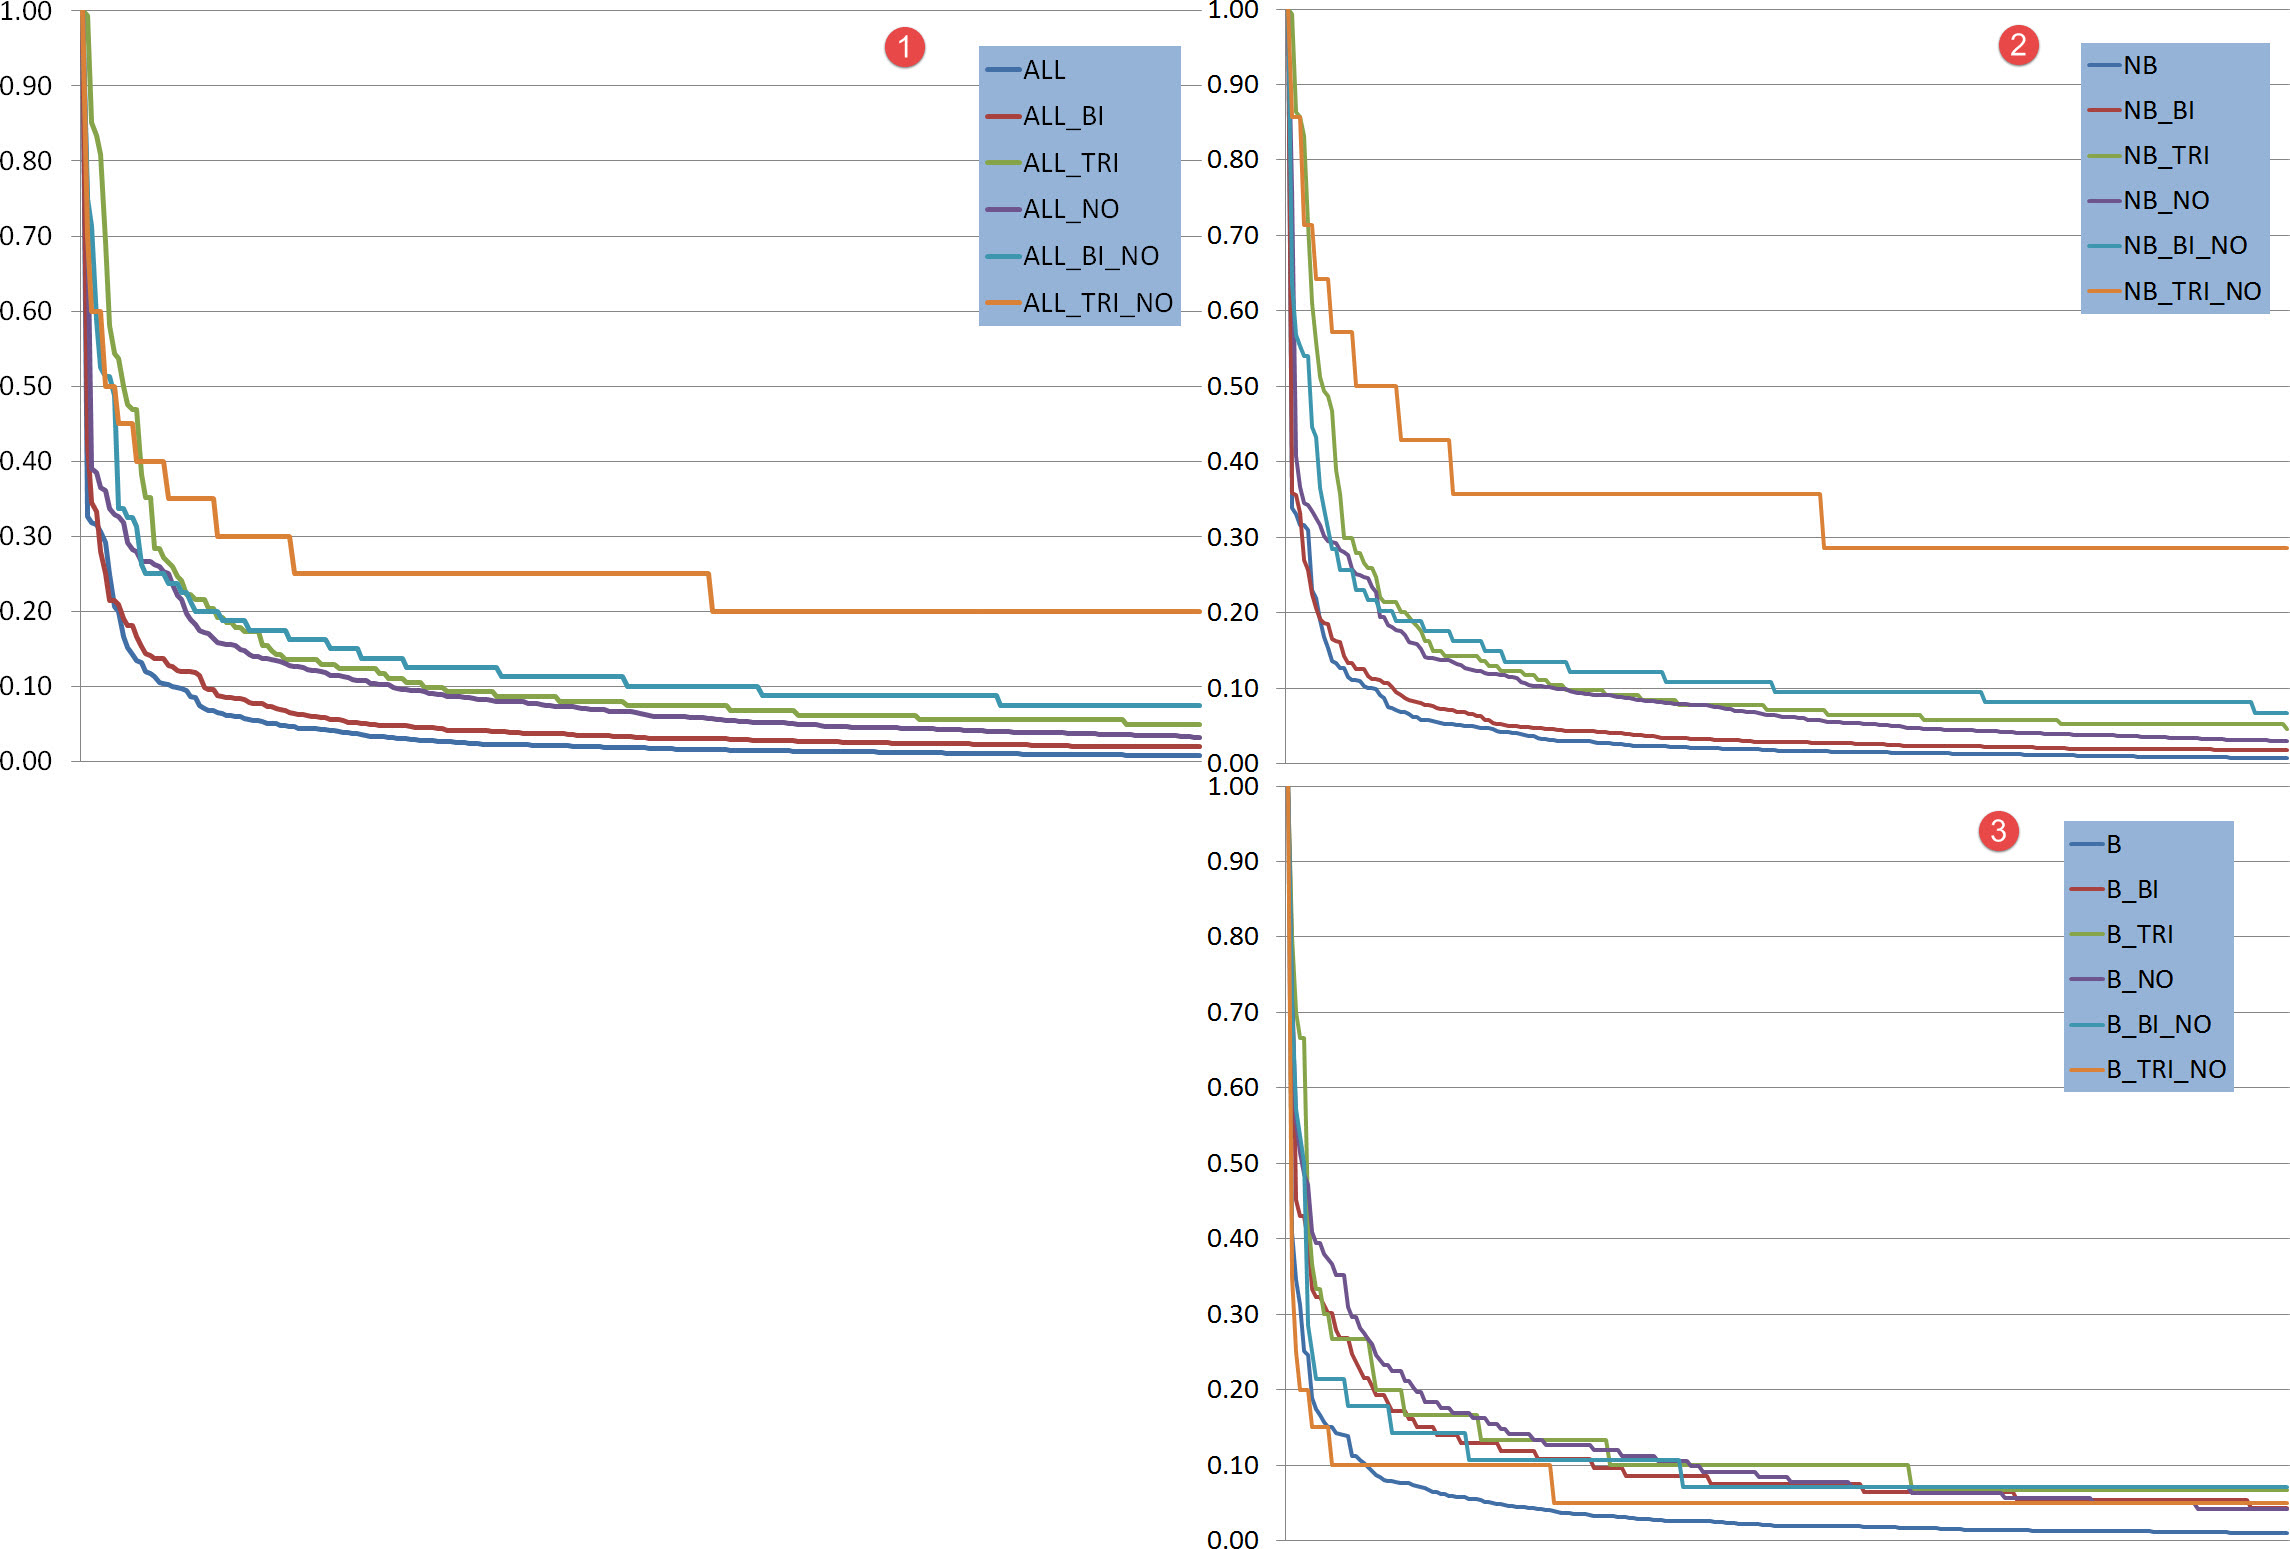
\includegraphics[width=1.0\textwidth]{Figures/Chapter4/word_frequencies.jpg}
	\caption[Normalised distribution of word frequencies]{Graphs showing the normalised word distribution of the different token configurations examined}
	\label{fig:chapter4:word_frequencies}
\end{figure}

Analysing these charts some observations can be immediately noted. Firstly the frequency distribution of tri-gram tokens for all words and for not bullying words, both with stop words removed, have a significantly different shape to all other frequencies. The frequency for not bullying bi-grams is particularly distinctive suggesting maybe that this list is more evenly distributed than the others. It was actually expected that the bullying trigrams would have proven the most evenly distributed dataset. However, the counts of the two most frequency occurring tokens, 20 and 7, when compared to the other frequency counts of 5 or less, meant that the distribution graph for this category fell off faster than any other.




\section{Data Preparation}
\label{section:data_prepatation}

With a better understanding of the data following its thorough exploration, the final step before modelling begins is to prepare the data. It would possible to include some of the processing of the data described here within the modelling process, for example converting case of all characters to lower case. However, it was decided that performing these steps in advance would allow better control and give greater transparency of the data submitted to classifier models. In this section, the processing or transformations performed are each described before discussing the reasons for each of them.

\subsection{Cleaning the Data}

In total eight transformation steps are applied to the data:

\begin{enumerate}
	\item Convert to lower case
	\item Convert to ASCII
	\item Remove URLs
	\item Remove all punctuation
	\item Replace numeric values 11 to 25 with text values
	\item Remove any digits that remain
	\item Remove any repeating characters
	\item Fix common abbreviations and replace with full word
\end{enumerate}

Python is once again the language of choice to perform these transformations. The data was read from the MySQL database in two blocks, the block of questions that were identified as bullying and the non bullying block. Instead of writing the final questions back to the database the questions were written to a file on disk for later processing by the Python Natural Language Toolkit (NLTK) \cite{bird_natural_2009} as described in Chapter \ref{chapter5}.

The first four transformations are conversion to lower case, the removal of non ASCII characters and URLs and the removal of any remaining punctuation characters. The complete scripts showing the details of how these string manipulations were performed are given in Appendix \ref{app:baseline}. The conversion of all text to lower case is a simple invocation of the \verb|lower| method on the question string which needs no further explanation. During data exploration, it was noticed that there were several characters that were not in the ASCII code set. The \verb|unicodedata.normalize| method shown on lines 28 to 32 of Appendix \ref{app:baseline} will return the normalised version of the passed string. The first parameter passed defines the decomposition to be applied to the Unicode string. Normal form KD (NFKD) will replace all compatibility characters with their equivalents. The string returned is encoded as ASCII. Next a standard regular expression representing a URL is used to remove all URLs by replacing them with an empty string, lines 35 to 38. 

Any remaining punctuation characters are removed next as shown on lines 41 to 45. The \verb|translate| string method takes two arguments. The first is a table of characters to translate, and the second is the list of characters to delete. \verb|string.maketrans| is used to create the table of characters to translate but when used as shown an empty table is created. The list of punctuation characters is passed as the second parameter. The effect of passing an empty table of translation characters and the list of punctuation characters is that the punctuation characters are just deleted which is the desired effect. The sixth transformation uses a slightly differently formatted version of the translate method but is used in the same manner to remove any remaining digits as shown on lines 52 and 53. Rather than passing the punctuation characters in this instance the lists of digits are passed, and \verb|None| represents an empty value in this case an empty table of translation characters.

The other three string manipulation routines replace selected numeric values with text, removes repeating characters and fix an identified number of abbreviations with whole words. From the data exploration, it was noticed that there were a number of bullying questions that requested sensitive personal information such as a persons age. To capture this important information, for use during the modelling process, a new class was developed to allow such a replacement. The details of this class are discussed shortly but the code to execute this substitution is given in lines 48 and 49 of Appendix \ref{app:baseline}. An instance of the \verb|RegexReplacerAge| is created and then the replace method is called on the passed string returning a new string where the required values have been replaced. The \verb|RegexReplacer| class used to replace common word abbreviations uses the same logic taking a string and returning the same string where occurrences of defined abbreviated words are expanded to their full representation.

The final piece of code to be examined is the code that removes repeating characters from the text of the questions. A \verb|RepeatReplacer| object is created as well as any empty array. Then for each word in the question, obtained using the split method, the replace method of the class is called returning a valid word without the repeating characters. The array of words created is then converted back to a string. 

The last three manipulation operations described rely on classes imported from a package in the same folder called \textit{``replacers.py''}. 

\begin{lstlisting}[]
from .replacers import RegexpReplacer
from .replacers import RegexpReplacerAge
from .replacers import RepeatReplacer
\end{lstlisting}

This replacer package is based on a package of the same name described in Python Text Processing with NLTK 2.0 Cookbook (\citet{perkins_python_2010}). The first class to consider is the \verb|RegexpReplacer| class. The core of this class is the \verb|replace()| method which takes a word and returns what is considered a more correct version. Before this class can be utilised an array of replacement patterns, or words, must first be defined. As shown in and Appendix \ref{app:replacer} the first three patterns are used to replace \textit{u} with the full word \textit{you}. For example \verb|(r'(\su\s)', ' you ')| searches the text for any occurrence of the letter u with white space (\verb|\s|) on both sides and replaces this with a space followed by the word ``you'' followed by another space. The two edge cases, where u is the first word in a question or the last word of the question are also handled. The \verb|$| symbol is used to identify the end of the text of the question and the \verb|^| symbol to identify the start of the question. 

The two most important concepts encapsulated in the class are performed by the \verb|re.compile| method and the \verb|re.subn| method. The compile method compiles the regular expression patterns, for example \verb|\su\s|, into a regular expression object. The subn method takes three parameters, the compiled regular expression object, the replacement text value and the string on which to perform the regular expression substitution. The resulting string and the number of substitutions made are returned. 

The \verb|RegexpReplacerAge| class is identical to the \verb|RegexpReplacer| class except that instead of taking text based patterns it is looking to replace digits that are representative of peoples ages. 

Just like the \verb|RegexpReplacer| class, the purpose of the \verb|RepeatReplacer| class, lines 115-130, is to return a more correct version of the word passed for processing. However, instead of replacing abbreviated words with the correct fully expanded word, the goal here is to remove unnecessary repeating characters. This class makes very good use of backreferences to remove these repeating characters. The \verb|repeat_regexp| regular expression will match zero or more characters at the start of the string and these are referenced as \verb|\1|. Next a single character is matched but it must be immediately followed by another instance of itself, referenced as \verb|\2|. Finally zero or more characters at the end of the string and these are referenced as \verb|\3|. Then \verb|repl| simply references \verb|\1 \2 \3| recombined without the single repeated character which is not included as it was not within the grouping parentheses of the second reference. The \verb|replace()| method is then called recursively to remove multiple repeated characters but makes use of a WordNet lookup as a stopping mechanism when a valid word is identified.

\subsection{Write Data in NLTK Corpus Format}

The Python script described in the previous section, shown in Appendix \ref{app:baseline}, was executed separately for questions classified as bullying and for questions classified as not bullying, the SQL on lines 18 and 19 was changed to select each class separately. Processing each class separately in this manner allowed each question to be written individually to a file in a folder named in accordance with the class type, for example bullying questions were written into a folder named \verb|bullying| and not bully question were written to a folder called \verb|not_bullying|. The parent folder for each was called \verb|01| as the dataset produced as a result of this processing will be called \verb|cyberbully_01| in later sections, the original raw data was written to disk in a similar manner without processing to a folder named \verb|00|. The name of the folder that the files were written to, lines 70 and 71, was changed to reflect the class that was being processed. Each question was written to a separate file that was anonymously named in the range \verb|00001| to \verb|99999| so that the question could not be traced back to the original question on the Ask.fm website. 

Once this \verb|01| dataset had been written to disk five further datasets were generated from it. Data \verb|02| and \verb|03| were the bi-grams and tri-grams datasets derived from the original \verb|01| dataset. Next, NLTK stop words were stripped from the \verb|01| dataset producing the \verb|11| dataset from which bi-grams and tri-grams were again generated producing datasets \verb|12| and \verb|13| respectively. The final structure of the NLTK corpora developed here can be seen in Figure \ref{fig:chapter5:corpus_structure}. All dataset manipulation was achieved using Python.

\subsection{Analysis of Cleaning Steps}

It is worth examining some of the changes made to the text of the questions by the processing described here, and explain the relevance of each step.

The conversion of all characters to lower case is a standard step to perform in text mining. The goal is to reduce the number of tokens that will later be presented to the model. For example, whilst the reader understands that \textit{``Why''}, \textit{``WHY''} and \textit{``why''} are all different representations of the same word. If presented to the text mining model in this manner, three distinct tokens will be identified. Interpreting words with different case representations as separate tokens increases the  size of the final word vector and also may have the unwanted side effect of either incorrectly diluting or multiplying the impact of a word in the generation of the classification model. Though capitalisation of words can be used to infer shouting or displeasure, for the purposes of this study it is acceptable that all words are converted to lower case.

Removal of non ASCII characters was performed to clean up the text of the question and remove extra characters added to ``beautify'' the question. It was also to ensure that all text was represented in its simplest form. This processing had the beneficial side effect, like the conversion to lover case, of standardising tokens. Examples of both the removal of unwanted characters and the standardising of text is shown in Figure \ref{fig:chapter4:remove_nonascii}. The first example shows how the non ASCII characters that spelt out the word \verb|beautiful| were converted into normal ASCII characters and the decorative symbols after the word were removed. The second example converted the phrase \verb|Love you Forever| to ASCII as well as removing the heart symbol.

\begin{figure}[htbp]
	\centering
	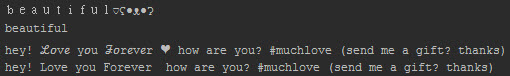
\includegraphics[width=0.85\textwidth]{Figures/Chapter4/remove_nonascii_01.jpg}
	\caption[Remove non ASCII characters]{Samples of where non ASCII characters were either removed or replaced with their ASCII equivalent}
	\label{fig:chapter4:remove_nonascii}
\end{figure}

It was decided that URL strings where so unique that they would not add any significant benefit if included in the model. They were stripped out wherever they were found. The removal of punctuation characters served at least two purposes. The first thing that stripping punctuation characters achieved was to remove all emoticons from the text of the questions. Although it could be argued that the emoticons are representative of the tone or sentiment of the question, it was observed that their use was inconsistent and there were multiple different representations of several emoticons. This all meant that the intended meaning of some emoticons were not obviously clear. In the first two examples shown in Figure \ref{fig:chapter4:remove_punct} it can be seen how removing the punctuation greatly cleans up the presentation of the text. The third examples shows the removal of two emoticons.

\begin{figure}[htbp]
	\centering
	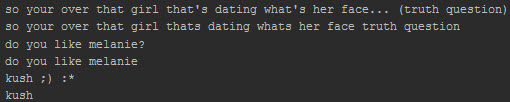
\includegraphics[width=0.85\textwidth]{Figures/Chapter4/remove_punct_01.jpg}
	\caption[Remove punctuation characters]{Samples of where punctuation has been removed showing where emoticons are removed}
	\label{fig:chapter4:remove_punct}
\end{figure}

Next it was decided to remove all numeric characters. However, it was noticed that there were a significant number of references to peoples ages and that most of these related to teenagers or early twenties. This information was considered useful and worth saving so before all other digits were removed the numbers from \textit{``11''} to \textit{``25''} inclusive were replaced with their text equivalent. After these numbers were substituted, all other digits were removed. A sample of an age being replaced with the text value is shown in \ref{fig:chapter4:remove_digit} as well as the removal of all other digits that are deemed not to represent ages.

\begin{figure}[htbp]
	\centering
	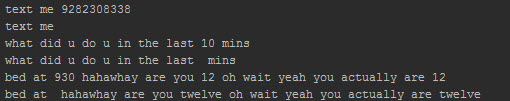
\includegraphics[width=0.9\textwidth]{Figures/Chapter4/remove_digits_01.jpg}
	\caption[Replace selected numerical ages with text then remove remaining digits]{Samples of where certain numbers have be substituted with text values and all other digits are removed}
	\label{fig:chapter4:remove_digit}
\end{figure}

As discussed earlier, the nature of social media means that text is often unstructured. Words are sometimes accentuated with the addition of extra repeated characters or abbreviated to their simplest forms. For example, \textit{``looove yoooou''} or \textit{``love u''} both mean the same thing but if left in this format extra unnecessary tokens will be added to the word vector diluting the effectiveness of the model. Alternatively, shorter tokens will be stripped because they do not meet a minimum token length criterion. In the first case the repeated characters are removed returning a valid word. In the second, a number of abbreviated words and their full text representations were defined. Sample of both these word manipulations can be seen in Figure \ref{fig:chapter4:remove_repeat}. The first two examples show the successful removal of repeated characters whilst the third example shows both repeated characters removed and the replacement of an abbreviated word with the correct word.

\begin{figure}[htbp]
	\centering
	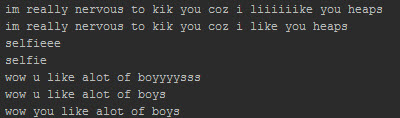
\includegraphics[width=0.75\textwidth]{Figures/Chapter4/remove_repeat_01.jpg}
	\caption[Remove repeated characters and abbreviated words]{Samples of where repeated characters have been removed and abbreviated words are replaced with correct word}
	\label{fig:chapter4:remove_repeat}
\end{figure}


\subsection{Data Exploration Revisited}

Now that \textit{``cleansed''} datasets are available for the not bullying and bullying classes it is worthwhile taking a brief step backwards and analyse these dataset using the same techniques described in Section \ref{section:data_exploration}. For brevity only the not bullying and bullying datasets are considered and only certain measures.

The top ten distinct token frequencies of bi-grams and tri-grams from the bullying dataset is shown in Table \ref{tab:chapter4:word_count_bullying_clean}. Looking first at bi-grams with stop words, eight out of the top ten tokens have not changed but what is noticeable is that overall the frequencies have increased. Looking at the bullying bi-grams with stop words removed only six of the original top ten are still present. Once again the frequencies have increased albeit more modestly. What is significant is that the previous number one most frequently occurring  bi-gram, \verb|right_now|, is now no longer included. Initially it was thought that this was an error, however, upon a more detailed examination it was discovered that the original two tokens were \verb|right| and \verb|now?|. The question mark character prevented \verb|now| from being identified as a stop word. It would appear that the cleaning process has impacted on bullying bi-grams. Whether this impact is positive or negative remains to be seen.

\begin{table}[h]
\centering
\caption[Distinct n-gram word counts (cleaned datasets)]{Table showing distinct counts of bi-gram and tri-gram tokens for the cleaned bullying dataset and also with and without stop words}
\label{tab:chapter4:word_count_bullying_clean}
\begin{tabular}{lrlr}
	\toprule
	\multicolumn{4}{c}{\textbf{Bullying Bi-Grams}} \\
	\cmidrule(r){1-4}
	\multicolumn{2}{c}{\textbf{With Stopwords}} & \multicolumn{2}{c}{\textbf{No Stopwords}} \\
    \midrule
	are\_you	&	155 & post\_pic		& 25	\\
	do\_you		&	106 & dont\_know	& 20	\\
	you\_have	&	65 & wearing\_right	& 20	\\
	you\_are	&	54 & dont\_like		& 13	\\
	of\_you		&	48 & cut\_cut		& 9	\\
	you\_and	&	47 & really\_pretty	& 9	\\
	what\_are	&	44 & post\_selfie	& 8	\\
	if\_you		&	42 & post\_picture	& 8	\\
	how\_old	&	37 & dont\_even		& 8	\\
	would\_you	&	36 & bra\_size		& 7	\\
    \bottomrule
    \end{tabular}
\begin{tabular}{lrlr}
	\toprule
	\multicolumn{4}{c}{\textbf{Bullying Tri-Grams}} \\
	\cmidrule(r){1-4}
	\multicolumn{2}{c}{\textbf{With Stopwords}} & \multicolumn{2}{c}{\textbf{No Stopwords}} \\
    \midrule
	what\_are\_you		& 36 &	cut\_cut\_cut			& 7 \\
	old\_are\_you		& 32 &	last\_person\_kissed	& 5 \\
	how\_old\_are		& 32 &	whoever\_likes\_thinks	& 4 \\
	are\_you\_wearing	& 22 &	see\_window\_post		& 4 \\
	you\_wearing\_right	& 20 &	seem\_really\_nice		& 4 \\
	wearing\_right\_now	& 20 &	window\_post\_pic		& 4 \\
	do\_you\_have		& 17 &	slept\_ex\_bf			& 3 \\
	are\_you\_single	& 17 &	shannon\_slept\_ex		& 3 \\
	of\_you\_and		& 16 &	likes\_thinks\_you're	& 3 \\
	are\_you\_doing		& 14  &	ex\_bf\_max				& 3 \\
    \bottomrule
    \end{tabular}
\end{table}

When the bullying tri-grams that included stop words were re-examined, eight of the top ten remained the same with high count frequencies evident. Surprisingly not only were nine of the top ten tri-grams where stop words had been removed the same as before the dataset was cleaned, but these nine tokens also had the same frequencies. The only token missing from the list was \verb|wearing_right_now| and as previously highlighted with the bi-grams this token is no longer occurring in the list because the genuine stop word \verb|now| is no longer available for consideration. It should be noted that further examination showed that this was not the only such occurrence of where a stop word had not been removed from the dataset because it was attached to a punctuation mark. It was again noticed that where stop words were not removed, personal pronouns were again a very common occurrence in the top ten list.

Table \ref{tab:chapter4:word_distribution_clean} shows the number of unique tokens in each of the cleaned datasets as well as the total count of tokens, and their average frequencies. The numbers in brackets show the percentage increase or decrease when compared with the original data. It is clear to see that nearly all counts are down and that, in general, the average frequencies have either increased or stayed the same. The general decrease in the number of tokens can be explained by the cleaning process where it was seen that many numerical tokens were removed, and multiple variations of the same token were standardised. The slight increase in the number of bullying n-grams with stop words is down to common abbreviations being standardised.

\begin{table}[h]
\centering
\caption[Unique tokens, total count and average frequency (cleaned datasets)]{Table showing the number of distinct tokens in each dataset as well as the total token counts and average frequencies}
\label{tab:chapter4:word_distribution_clean}
\begin{tabular}{lrrl}
	\toprule
	{\textbf{Token}} 		& {\textbf{Unique}} & {\textbf{Total}} & {\textbf{Average}}  \\
	{\textbf{description}}	& {\textbf{Tokens}} & {\textbf{Count}} & {\textbf{Frequency}}  \\
    \midrule
    \midrule
    \multicolumn{1}{l}{\textbf{Not Bullying}} \\
	\cmidrule(l){1-1}
	Uni-Grams					& 6579 (-37\%) &	61293 (-13\%)	& 9.1 (+39\%) \\
	Bi-Grams					& 29149 (-13\%) &	53436 (-13\%)	& 1.8 (same)\\
	Tri-Grams					& 38701 (-5\%) &	46120 (-13\%)	& 1.2 (-8\%) \\
	Uni-Grams No Stop Words		& 6462 (-38\%) &	33156 (-19\%)	& 5.1 (+31\%) \\
	Bi-Grams No Stop Words		& 21172 (-16\%) &	25394 (-20\%)	& 1.2 (-8\%) \\
	Tri-Grams No Stop Words		& 18311 (-14\%) &	18746 (-21\%)	& 1.0 (-9\%) \\
    \midrule
    \midrule 
    \multicolumn{1}{l}{\textbf{Bullying}} \\
	\cmidrule(l){1-1}
	Uni-Grams					& 2568 (-29\%) &	15323 (+1\%)	& 6.0 (+43\%) \\
	Bi-Grams					& 9039 (-9\%) &	13679 (+1\%)	& 1.5 (+7\%) \\
	Tri-Grams					& 10809 (+3\%) &	12112 (+1\%)	& 1.1 (same)\\
	Uni-grams No Stop Words		& 2459 (-30\%) &	8312 (-8\%)	& 3.1 (+31\%) \\
	Bi-Grams No Stop Words		& 5993 (-12\%) &	6676 (-10\%)	& 1.1 (same)\\
	Tri-Grams No Stop Words		& 5190 (-11\%) &	5282 (-11\%)	& 1.0 (same)\\
    \bottomrule
    \end{tabular}
\end{table}

Finally, in Figure \ref{fig:chapter4:word_frequencies_clean}, the normalised word frequencies for the cleaned datasets are shown. When compared to the earlier graph in Figure \ref{fig:chapter4:word_frequencies} differences are not immediately obvious. On closer examination of the not bullying graph, labelled (1), it is clear that the distribution of the bi-grams is more uniformly spread out and that the tri-gram distribution is closer to the other datasets. The most obvious difference in the bullying graph, (2), is the affect on the tri-gram distribution following the removal of the most frequently occurring token.

\begin{figure}[!htb]
	\centering
	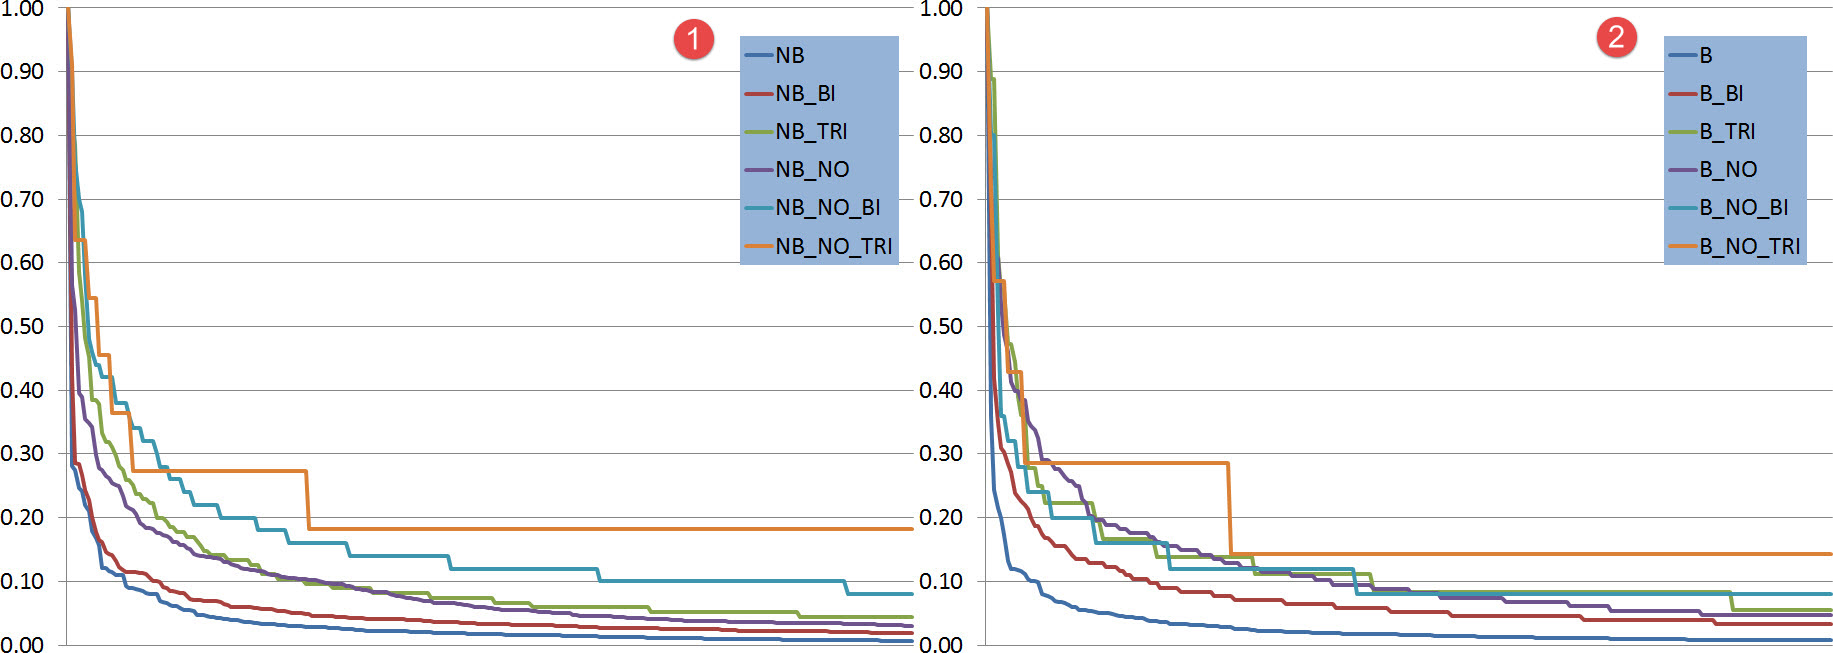
\includegraphics[width=1.0\textwidth]{Figures/Chapter4/word_frequencies_clean.jpg}
	\caption[Normalised distribution of word frequencies]{Graphs showing the normalised word distribution of the different token configurations examined}
	\label{fig:chapter4:word_frequencies_clean}
\end{figure}

\subsection{Data Visualisation Revisited}

Word clouds were also generated for bi-grams and tri-grams and the results can be seen in Figure \ref{fig:chapter4:bi-grams_wordclouds} and Figure \ref{fig:chapter4:trigram_wordclouds}. The many Eyes website was used once again with the same settings as before.

\begin{figure}[!htb]
	\centering
	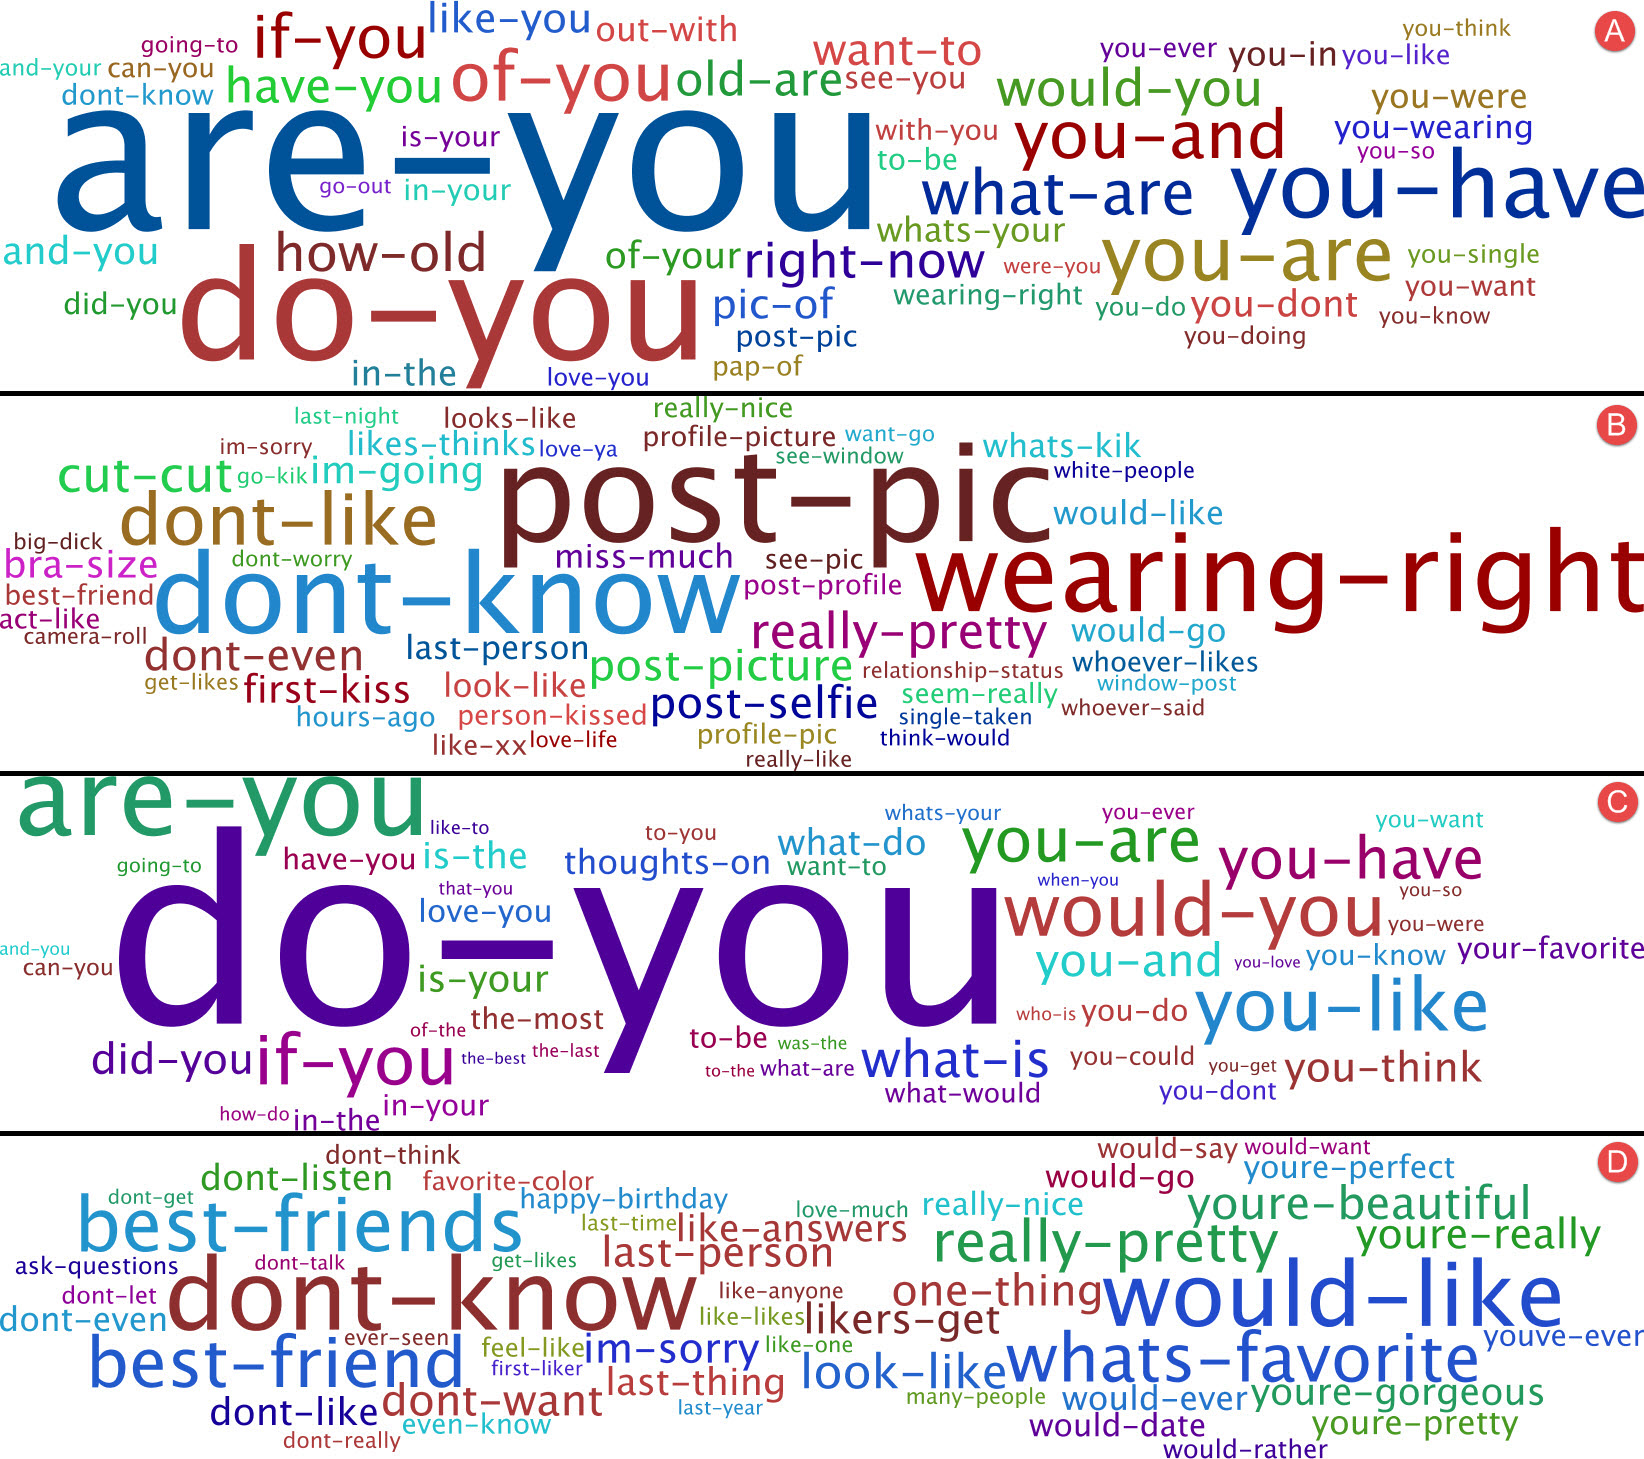
\includegraphics[width=1.0\textwidth]{Figures/Chapter4/bigram_clouds.jpg}
	\caption[Bi-gram word clouds]{Word clouds showing bullying bi-grams (a), bullying bi-grams with stop words removed (b), not bullying bi-grams (c) and not bullying bi-grams with stop words removed (d)}
	\label{fig:chapter4:bi-grams_wordclouds}
\end{figure}

\begin{figure}[!htb]
	\centering
	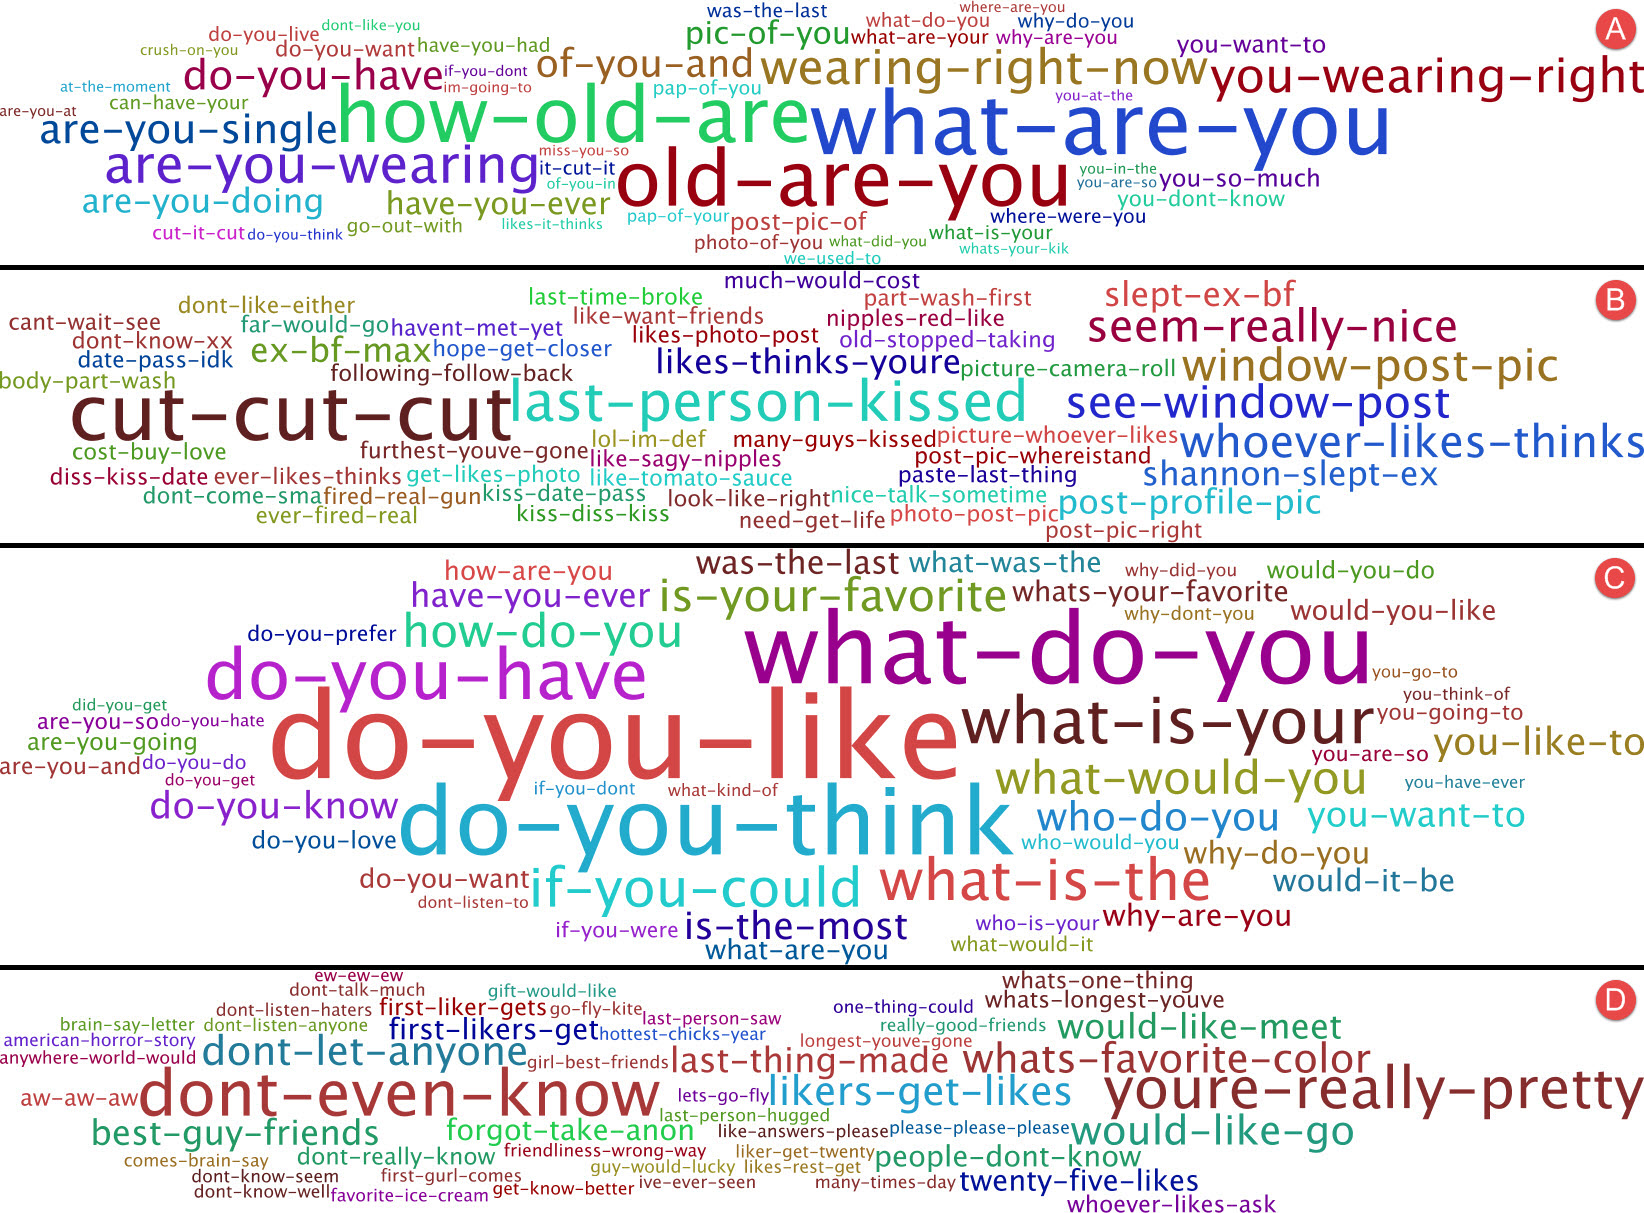
\includegraphics[width=1.0\textwidth]{Figures/Chapter4/trigram_clouds.jpg}
	\caption[Tri-gram word clouds]{Word clouds showing bullying tri-grams (a), bullying tri-grams with stop words removed (b), not bullying tri-grams (c) and not bullying tri-grams with stop words removed (d)}
	\label{fig:chapter4:trigram_wordclouds}
\end{figure}

As was seen with uni-grams the word clouds are dominated by stop words, especially the personal pronoun you. Looking at bi-grams first in Figure \ref{fig:chapter4:bi-grams_wordclouds}, the most frequently occurring bullying and not bullying tokens, \textit{``are\_you''} and \textit{``do\_you''}, are easily seen in section A and section C. Even after stop word removal, section B and section D, the bi-grams with the highest frequency occurrences are still clearly visible. Examining the tri-gram word clouds in Figure \ref{fig:chapter4:trigram_wordclouds} it is obvious that the tokens are now more evenly distributed. Even though the frequency of these bullying and not bullying tokens are more evenly distributed, when compared to uni-grams and bi-gram clouds, there are still a number prominent tokens. It is hoped that these tokens would be good predictors for both class types.




\section{Summary and Conclusion}
\label{section:summary_conclusion}

This chapter focused on the data. In the next chapter this data will be mined to develop a model to classify a question as either bullying or not bullying. 

In Section \ref{section:data_extraction} an overview of how the data was obtained from the Ask.fm site was given. A sample block of data, the question, answer and other meta data was shown and explained. The criteria used to determine which data was to be scraped, and the method used to extract it, was given. The data was then obtained over a twenty-four hour period in an attempt to make sure that the users from which the data was scraped covered as many geographical areas as possible and were not, for example, all from a single time zone. Upon completion of this task 110,000 data examples had been obtained.

Section \ref{section:initial_processing} described how the raw data extracted from the Ask.fm website was transformed into text more suitable for text mining. The original HTML format of the data was given and then the Python used to transform this into text was detailed. The Python \verb|glob| and \verb|os| packages were used to access the HTML files and Beautiful Soup, a Python library for parsing HTML documents, was used to parse these files so that the individual data elements described could be extracted. In total seven attributes were extracted per record. The data was loaded into a MySQL database. To complete the preprocessing the data was divided into three separate groups.  10\% for classification and model training and test, 80\% to simulate a stream of data arriving at the ask.fm website and a final block of 10\% for validation purposes. 

Section \ref{section:data_classification} gave an overview of the process used in the classification of each question as being either bullying or not bullying and also included detailed descriptions of the various types and categories of cyberbullying to be identified. Samples of some of the questions classified as bullying were also shown. Just under 11,000 sample questions were classified.

In Section \ref{section:data_exploration} a more detailed description of the data was given. It was noted that the structure of the data is relatively simple. Next some data quality issues were highlighted including non ASCII characters, slang words, abbreviations, repeated characters and emoticons. The section also included a detailed exploration of the dataset and also some word cloud visualisations and word, or token, frequency analysis.

In the final section, Section \ref{section:data_prepatation}, the data underwent a series of transformations in order to clean the data in preparation for modelling. As before Python was used to process the text of the dataset and in all eight cleansing steps were performed. The data was then written out to  files in NLTK corpora format.



%-------------------------------------
%	CHAPTER 5
%-------------------------------------
% Chapter Template

\chapter{Data Modelling} % Main chapter title

\label{chapter5} 

\lhead{Chapter 5. \emph{Data Modelling}} 

The focus of this chapter is to describe the process to develop the best model for predicting whether a question from the Ask.fm website could be considered as either bullying or not bullying. The modelling approach is given, and it also highlights any alterations that were required to be made to this initial plan. However, before going into the detail of the modelling approach there is a brief refresher of the data available and its structure.

At the completion of Chapter \ref{chapter4}, where the data extracted from the Ask.fm website was explored and processed, a number of datasets were now available for modelling. In total seven datasets were generated:

\begin{enumerate}

	\item The original raw question data as extracted from Ask.fm [dataset 00]
	\item The cleaned version of the original dataset [dataset 01] (considered the primary dataset)
	\item Bi-grams created from the cleaned dataset [dataset 02]
	\item Tri-grams created from the cleaned dataset [dataset 03]
	\item The cleaned dataset with all NLKT stop words removed [dataset 11]
	\item Bi-grams created from the cleaned dataset with all NLKT stop words removed [dataset 12]
	\item Tri-grams created from the cleaned dataset with all NLKT stop words removed [dataset 13]

\end{enumerate}

All seven datasets were written to the NLTK data folder as separate corpora. 

A description of the initial first modelling attempts using the Natural Language Toolkit (NLTK) are given in Section \ref{subsection:nltk-initial_modelling}. Here a Naive Bayes classifier is used to gain insight into the potential predictive performance of a model when classifying the text. As well as examining the performance of each of the datasets generated in Chapter \ref{chapter4}, this section also analyses whether the N-gram generation and stop word removal functionality natively available in the NLTK performs any better or worse. 

Next, in Section \ref{subsection:nltk-class_imbalance}, ways to address the minority positive class and majority negative class imbalance are explored. Techniques utilised include under sampling of the majority class, over sampling of the minority class and a hybrid approach that uses both under and over sampling. Also explored is whether only selecting a percentage of the most frequently occurring tokens in each class makes a difference to the performance of any models generated. Once again a basic NLTK Naive Bayes model is applied.

Sections \ref{subsection:scikit-learn} and \ref{subsection:scikit-class-imbalance} then repeat the modelling processes undertaken in Sections \ref{subsection:nltk-initial_modelling} and \ref{subsection:nltk-class_imbalance} but using the Scikit-Learn Python libraries. In these sections a Linear Support Vector classifier is used in addition to a Naive Bayes. Section \ref{subsection:scikit-learn-cost} investigates the possible use of a cost sensitive approach to modelling before the best models developed are identified in Section \ref{subsection:best-classifiers}. Finally in Section \ref{subsection:applying-classifiers} the three best models identified are further tested using previously unseen data. Using the top three models a hold back dataset is classified. The models then evolve using a third dataset and the hold back dataset is classified and the results analysed. 
\section{Natural Language Toolkit - Initial Modelling}
\label{subsection:nltk-initial_modelling}

The first model was developed using the primary dataset, data that has been cleansed but stop words have not been removed, and the Python NLTK. A Naive Bayes learner using a feature based bag of words approach was chosen. The data was stored in the NLTK corpus format where each question was individually written to a file in a folder that represented whether it was classified as bullying or not bullying. For reference, this structure is shown in Figure \ref{fig:chapter5:corpus_structure}

\begin{figure}[htbp]
	\centering
	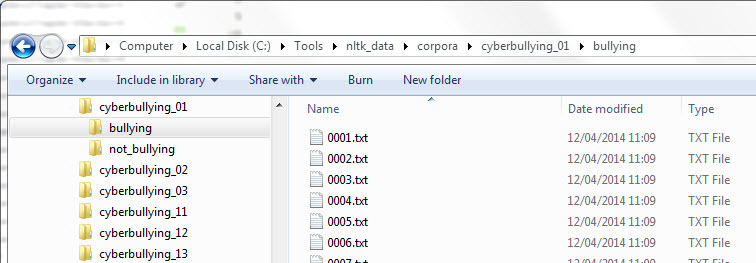
\includegraphics[width=0.85\textwidth]{Figures/Chapter5/corpus_structure.jpg}
	\caption[The structure of the primary datset corpus]{The structure of the primary dataset is shown with the top level folder containing a folder for the bullying questions and the not bullying questions. A file per question is created.}
	\label{fig:chapter5:corpus_structure}
\end{figure}

\subsection{Model Development}

The development of a NLTK classifier model is a relatively straight forward task. The first step is to create a categorised plain text corpus reader. The reader takes three parameters. The first parameter is the root folder for the corpus, the second is a regular expression used to identify the files in the corpus, the third is a regular expression used to determine the category names which are derived from the folder names within the corpus. In the code snippet shown in Listing \ref{lst:chapter5.1:snipet_01}, lines 1 to 5, the corpus to be read is \verb|cyberbullying_01| and all files with a \verb|.txt| extension are included. Now that the reader is initialised the next step is to identify the file ids of each category type.

\begin{lstlisting}[caption={Creating the categorised plain text corpus reader},label=lst:chapter5.1:snipet_01]
# Set the working folder to the nltk_data corpora folder
os.chdir ('c:/Tools/nltk_data/corpora')
reader = CategorizedPlaintextCorpusReader('./cyberbullying_01',
                                          r'.*\.txt',
                                          cat_pattern=r'(\w+)/*')
\end{lstlisting}

Identifying the file ids of each category is just a matter of calling the \verb|fileids| method passing the category name of the required file ids. The code snippet in Listing \ref{lst:chapter5.1:snipet_02} returns two file lists the first, \verb|pos_ids| is a list of all the files, including each files relative path, in the positive or bullying category while the \verb|neg_ids| is the list of all files in the negative or not bullying category. 

\begin{lstlisting}[caption={Identifying the positive and negative file ids},label=lst:chapter5.1:snipet_02]
# The questions containing bullying are the positive tests
pos_ids = reader.fileids('bullying')

# The questions not containing bullying are the negative tests
neg_ids = reader.fileids('not_bullying')
\end{lstlisting}

Figure \ref{fig:chapter5:pos_ids} is a screen capture showing the first nine files in the positive, bullying, category and that there are 1,644 files in this category. There are 7,899 files in the negative or not bullying category.

\begin{figure}[htbp]
	\centering
	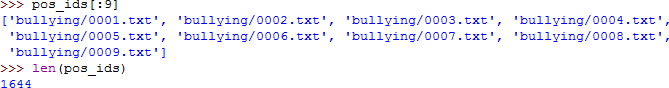
\includegraphics[width=1\textwidth]{Figures/Chapter5/pos_ids.jpg}
	\caption[List of files for the bullying category]{Screen capture showing the first nine files in the positive, bullying, category and also that there are 1,644 files in this category}
	\label{fig:chapter5:pos_ids}
\end{figure}

The NLTK uses the concept of a feature, in this case a word or token, and the Naive Bayes Classifier in the NLTK operates solely on whether a feature is present in a sample or not. The code in Listing \ref{lst:chapter5.1:snipet_03} shows how the positive and negative feature dictionaries are generated. The first three positive features are shown in Figure \ref{fig:chapter5:pos_feat} with the second sample highlighted to help distinguish each sample. Examining this second sample further, it can be seen that it is a Python dictionary containing fourteen words where each value has been given a value of true to signify their presence in the sample. Each sample is also categorised as bullying. It should be noted that all sentence word order has been lost as would be expected when using a bag of words approach. A similar process is performed to created the negative features. 

\begin{lstlisting}[caption={Generation of the positive and negative feature dictionaries},label=lst:chapter5.1:snipet_03]
def word_feats(words):
    return dict([(word, True) for word in words])

pos_feat = [(word_feats(reader.words(fileids=[f])),
             'bullying')
            for f in pos_ids]

neg_feat = [(word_feats(reader.words(fileids=[f])),
             'not_bullying')
            for f in neg_ids]
\end{lstlisting}

\begin{figure}[htbp]
	\centering
	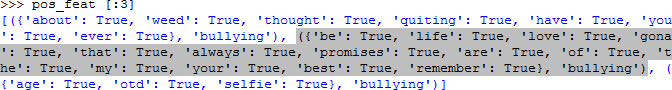
\includegraphics[width=1\textwidth]{Figures/Chapter5/pos_feat.jpg}
	\caption[Sample positive features]{Screen capture showing the first three positive features}
	\label{fig:chapter5:pos_feat}
\end{figure}

Next, the Naive Bayes learner is trained and it's performance calculated. Unfortunately, NLTK does not natively support cross validation. This meant that ten-fold cross validation had to be manually implemented in code. Full details of the implementation of the cross validation can be seen in Appendix \ref{app:simple_nltk}. Using a simple cross validation solution, the positive and negative samples were divided into ten parts. Nine of the positive and negative parts were joined together to create the training dataset and the remaining positive and negative parts joined to create the test dataset. A Naive Bayes classifier was then created using the training dataset as shown in Listing \ref{lst:chapter5.1:snipet_04}. Also shown, lines 4 - 8, is the generation of a reference set and test set to be used to calculate the performance of the classifier. To achieve this the actual classification of each of the test samples is loaded into the reference set and the value for the sample returned from the classifier is loaded into the test set. Then, using the NLTK metrics package, the performance of the classifier is calculated. For example, line 12 shows the calculation of the precision for the positive bullying samples. Finally line 18 will display the top 5 most informative features of the classifier.

\begin{lstlisting}[caption={Generation of the positive and negative feature dictionaries},label=lst:chapter5.1:snipet_04]
# Create the classifier using the train dataset
classifier = NaiveBayesClassifier.train(train)
 
#Populate the metrics sets with values
for i, (feats, label) in enumerate(test):
    refsets[label].add(i)
    observed = classifier.classify(feats)
    testsets[observed].add(i)
        
# Calculate precision. recall, f-measure
#   and accuracy
pos_pre  += nltk.metrics.precision(refsets['bullying'],
                                   testsets['bullying'])
...
# Show the top 5 most informative features
classifier.show_most_informative_features(5)
\end{lstlisting}

Once the cross validation testing has been completed then the average performance measures are calculated. A simplified visual representation of the process used to develop the first model using the NLTK is shown in Figure \ref{fig:chapter5:nltk_process_01}

\begin{figure}[htbp]
	\centering
	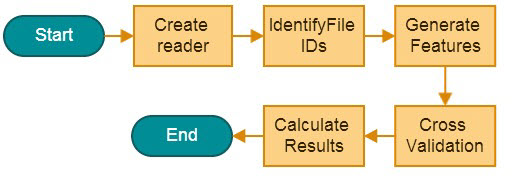
\includegraphics[width=0.85\textwidth]{Figures/Chapter5/nltk_process_01.jpg}
	\caption[NLTK model development process]{Simplified visual representation of the process used to develop the first model using the NLTK}
	\label{fig:chapter5:nltk_process_01}
\end{figure}

\subsection{Model Execution and Performance}

The NLTK Naive Bayes classifier described is then run on the primary dataset. The performance results and top five most informative features of the tenth cross validation run are shown in the screen capture in Figure \ref{fig:nltk_process_results_01}

\begin{figure}[htbp]
	\centering
	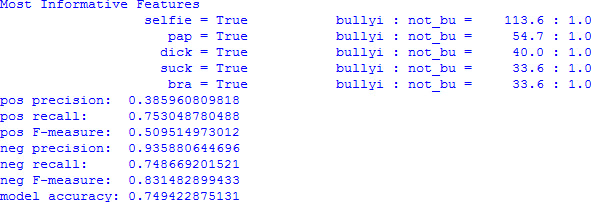
\includegraphics[width=.85\textwidth]{Figures/Chapter5/nltk_process_results_01.jpg}
	\caption[Performance measurements for initial NLTK classifier]{Screen capture of the top five most informative features from the tenth cross validation run and also the overall performance measurements for the NLTK classifier}
	\label{fig:nltk_process_results_01}
\end{figure}

Considering the top five most informative features, it is clear that these tokens, real words in this example, could easily be included in a question that was bullying in nature. The overall average accuracy of the model, just under 75\%, could suggest that this was a very successful first attempt at developing a model to predict bullying. However, looking closely at the precision and the recall for the different classes this is clearly not the case. The negative class precision, 93.6\%,  shows that nearly every sample classified as not bullying was an actual not bullying sample. Add to this a negative class recall value of 74.8\% and the model correctly identified nearly three out of every four not bullying questions. Examining the positive class next a recall value is seen which, at 75.3\%, shows that three-quarters of all bullying questions were correctly identified. However, a precision value of just 38.6\% shows that only two out of every five samples classified as bullying were  bullying questions implying that three out of every five samples classified as bullying were, in fact, not bullying questions. 

The model developed was then run on all seven datasets. The performance results for each dataset are shown in Figure \ref{fig:nltk_process_chart_01}.

\begin{figure}[htbp]
	\centering
	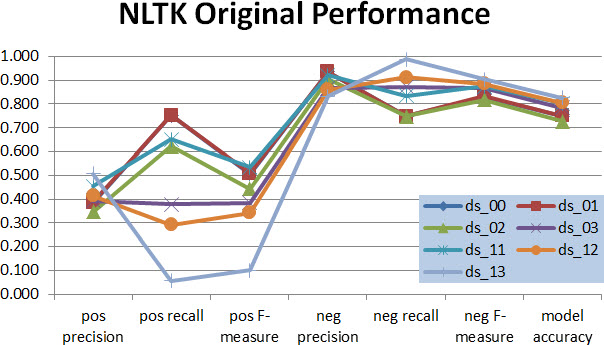
\includegraphics[width=.75\textwidth]{Figures/Chapter5/nltk_process_chart_01.jpg}
	\caption[Initial NLTK model performance across datasets]{Graph showing the performance of the initial NLTK Naive Bayes model across the seven manually crafted datasets}
	\label{fig:nltk_process_chart_01}
\end{figure}

\subsection{Model Analysis}
The first observation from an analysis of the data is that the precision of the model in predicting the positive class, the bullying questions, is poor when compared to the values obtained for the negative class with an average value of 41\% compared to an average value of 89\%. Although the average performance for recall for the positive class is 50\% this figure is not representative because of the value achieved for \verb|ds_13|, tri-grams with stop words removed, which is less than 10\%. 

Taking all performance measures into account, it could be said that the best performance achieved by this model was with \verb|ds_11|, uni-grams with stop words removed. However, with a precision value for the positive class of 45.3\% and a recall value of 65.2\% the results are far from satisfactory. This was just an initial modelling attempt and there are many changes that could be made to this model to improve its performance. Addressing class imbalance, only selecting the features that have the highest impact and by changing from the feature based approach offered by NLTK to the more statistical TF-IDF implementation offered by the Scikit-Learn package are some of the options to consider. It should also be noted that the Scikit-Learn package comes with its own cross validation implementation which will lead to a simplification of the code used.

\subsection{Further Exploration}

Before leaving this first simple model it was decided to determine if there was any advantage gained, or different results achieved, by generating the bi-grams and tri-grams up front. To test this, a simple change was needed to the \verb|word_feats| function to return bi-grams or tri-grams. Returning bi-grams is shown in Listing \ref{lst:chapter5.1:snipet_05}. Four new models were created using the bi-grams and tri-grams datasets generated from \verb|dataset_01| and \verb|dataset_11|.

\begin{lstlisting}[caption={Generation of the positive and negative feature dictionaries},label=lst:chapter5.1:snipet_05]
from nltk import bigrams
from nltk import trigrams
...
def word_feats(words):
    return dict([(word, True) for word in bigrams(words)])
\end{lstlisting}

The results generated by these new models were then compared to the original models where the bi-gram and tri-gram tokens were manually created beforehand. The different models were compared in three areas. The first, and easiest to compare, was average execution time. The average run time for each model was determined and it was found that generating the bi-grams or tri-grams during model execution did add to the overall execution time as can be seen in Table \ref{tab:chapter5:ngram_generation}. With a maximum time of 0.1 seconds to generate all tri-grams in advance, the longest to create, it is clear that there is a time advantage to creating all n-grams upfront. In Table \ref{tab:chapter5:ngram_generation} the first column is the model execution where the n-grams were generated before hand. Thee second column is the time for n-grams created during model execution. Column three is the time difference in seconds and the fourth column is the percentage increase in time.

\begin{table}[h]
\centering
\caption[N-gram generation increases execution time]{Table showing average model execution time increase when n-grams are generated as part of the modelling process}
\label{tab:chapter5:ngram_generation}
\begin{tabular}{rrrrr}
	\toprule
     & \textbf{orig}  & \textbf{new} & \textbf{diff} & \textbf{percent}    \\
    \midrule
    bi-gram & 19.399 & 20.549 & 1.150 & 5.9\%  \\
    tri-gram & 23.116 & 24.647 & 1.531 & 6.6\%  \\
    bi-gram ns & 14.357 & 15.685 & 1.328 & 9.3\%   \\
    tri-gram ns & 11.477 & 14.225 & 2.748 & 23.9\%   \\
    \bottomrule
    \end{tabular}
\end{table}

The second comparison is the performance of the models. The results of this analysis is shown in Figure \ref{fig:nltk_process_chart_02}. A cursory look at these charts  shows that the generation of the n-grams during the model execution did not improve the overall performance of the model. It may, it fact, have had a slightly negative impact which can be seen in the positive class recall and f-measure values. In all charts the top line in the legend represents the performance of the original model. For example, in the chart labelled ``Bi-grams no stop words'', the \verb|01_12| series, represented by the blue line shows, the performance values of the original model, \verb|01|, using bi-grams generated from the dataset where stop words have already been removed, \verb|_12|. The orange line, \verb|02_12|, is from the second model where bi-grams were generated during model execution.

\begin{figure}[htbp]
	\centering
	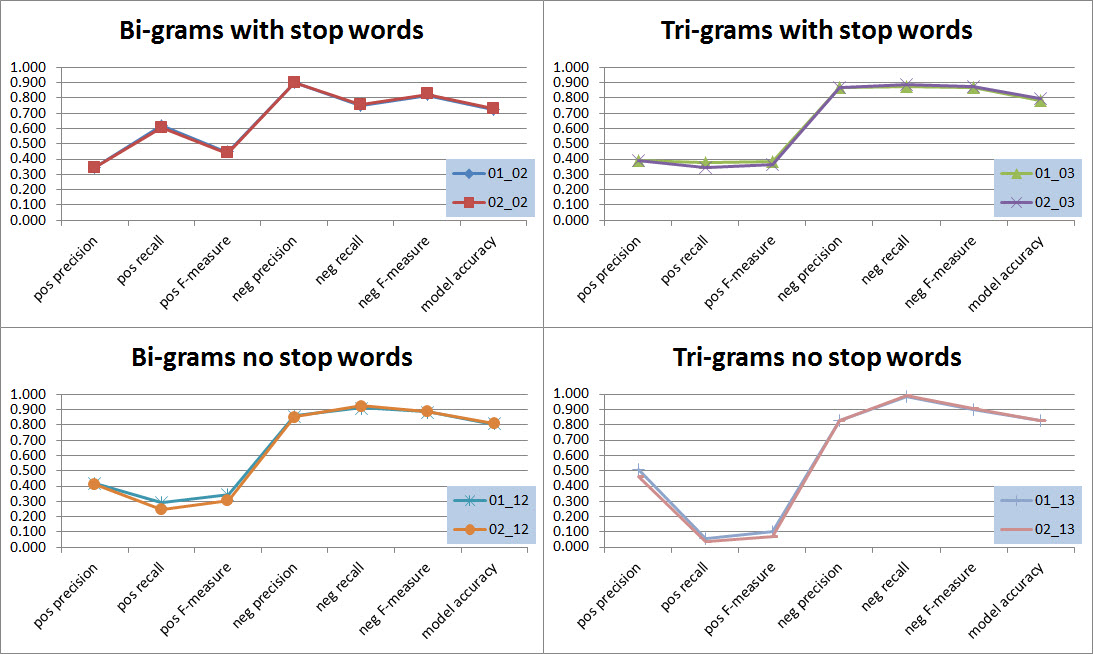
\includegraphics[width=1\textwidth]{Figures/Chapter5/nltk_process_chart_02.jpg}
	\caption[Comparison of pre-generated and in model n-gram generation]{Graphs showing a comparison or model performance when n-grams are pre-generated or generated during model execution}
	\label{fig:nltk_process_chart_02}
\end{figure}

The final analysis performed was a comparison of the most informative features returned during each model execution. Ten-fold cross validation was used and the top five most informative features were returned. The results of the number of most informative features comparison is summarised in Table \ref{tab:chapter5:informative_features}.

Whilst initially it appeared that there were a number of significant differences, after an investigation it was found that sometimes the most informative features with the same ratio values were sorted differently between the two model types. The other cause of the differences was the way the datasets were processed when the n-grams were generated during execution. When the tri-grams were generated up front, samples that had only two words never got included in the datasets submitted to the modelling process. This meant that there were only 1,049 positive and 4,915 negative samples for tri-grams with no stop words. However, there are 1,637 and 7,800 samples respectively in the uni-grams with no stop words dataset. As the ten-fold cross validation datasets were created before the n-grams were generated, this lead to a different split of the samples in the two models being compared. 

\begin{table}[h]
\centering
\caption[Most informative feature comparison]{Table showing the number of the most informative features that were different when n-grams were generated during model execution using the NLTK compared to being generated beforehand}
\label{tab:chapter5:informative_features}
\begin{tabular}{rc}
	\toprule
    \textbf{Model} & \textbf{Number} \\
    \textbf{Type} & \textbf{Differences} \\
    \midrule
    Bi-grams & 5 \\
    Tri-grams & 2   \\
    Bi-grams no stop words & 3    \\
    Tri-grams no stop words & 15    \\
    \bottomrule
    \end{tabular}
\end{table}

Based on the analysis given it was decided that for the simple NLTK model developed here it did not matter that the n-gram datasets were generated beforehand. It should be noted, however, that the models generated used all the classified data available and they were not tested on unseen data. This is not considered an issue as the performance results achieved here will be considered as a baseline against which all subsequent models could be compared.
\section{Natural Language Toolkit - Class Imbalance}
\label{subsection:nltk-class_imbalance}

It was observed that there was a class imbalance between the positive and negative samples. In this section, it will be investigated if over sampling the minority positive class or under sample the majority negative class affects the performance of the model. A compromise solution where the positive class is partially over sampled and the negative class is partially under sampled is also examined. More advanced methods for handling class imbalance such as cost based learners or the Synthetic Minority Over-sampling Technique (SMOTE) are not suitable for consideration at this time using the NLTK datasets. Although not strictly a class imbalance solution, sampling using the most frequently observed features is also explored.

\subsection{Majority Class Under Sampling}
Under sampling of the majority negative class was first to be explored. In all NLTK datasets the ratio of negative to positive classes is between 4:1 and 5:1. To determine how different negative class to positive class ratios affect the model performance, under sampling of the majority class at ratios of 3:1, 2:1 and 1:1 to the minority class will be examined.

To implement the desired ratios, the Python script described in Section \ref{subsection:nltk-initial_modelling} requires one minor change as shown in Listing \ref{lst:chapter5.2:snipet_01}. The file ids of the not bullying, or negative class, are read into the \verb|all_neg_ids| list. The order of the file ids are then shuffled and the required ratio is achieved by only taking multiples of the number of positive ids as required. In line 6 the ratio of negative to positive samples is 3:1. 

\begin{lstlisting}[caption={Adjust the postive to negative class ratio}, label=lst:chapter5.2:snipet_01]
# The questions not containing bullying are the negative tests
all_neg_ids = reader.fileids('not_bullying')

# Shuffle the file ids of the negative file
random.shuffle(all_neg_ids)
neg_ids = all_neg_ids[:len(pos_ids)*3]
\end{lstlisting}

The NLTK Naive Bayes model was generated five times for each dataset and average performance values calculated. Because the negative samples are randomly chosen, it was important to run multiple executions for each dataset to allow for any possible variance or imbalance in the samples selected. It was found that five executions were enough to show that all results were similar and consistent. The performance results achieved for each dataset at ratios of 3:1, 2:1, 1:1, and the original performance measures from Section \ref{subsection:nltk-initial_modelling}, are shown in Figure \ref{fig:nltk_process_chart_03}.

\begin{figure}[htbp]
	\centering
	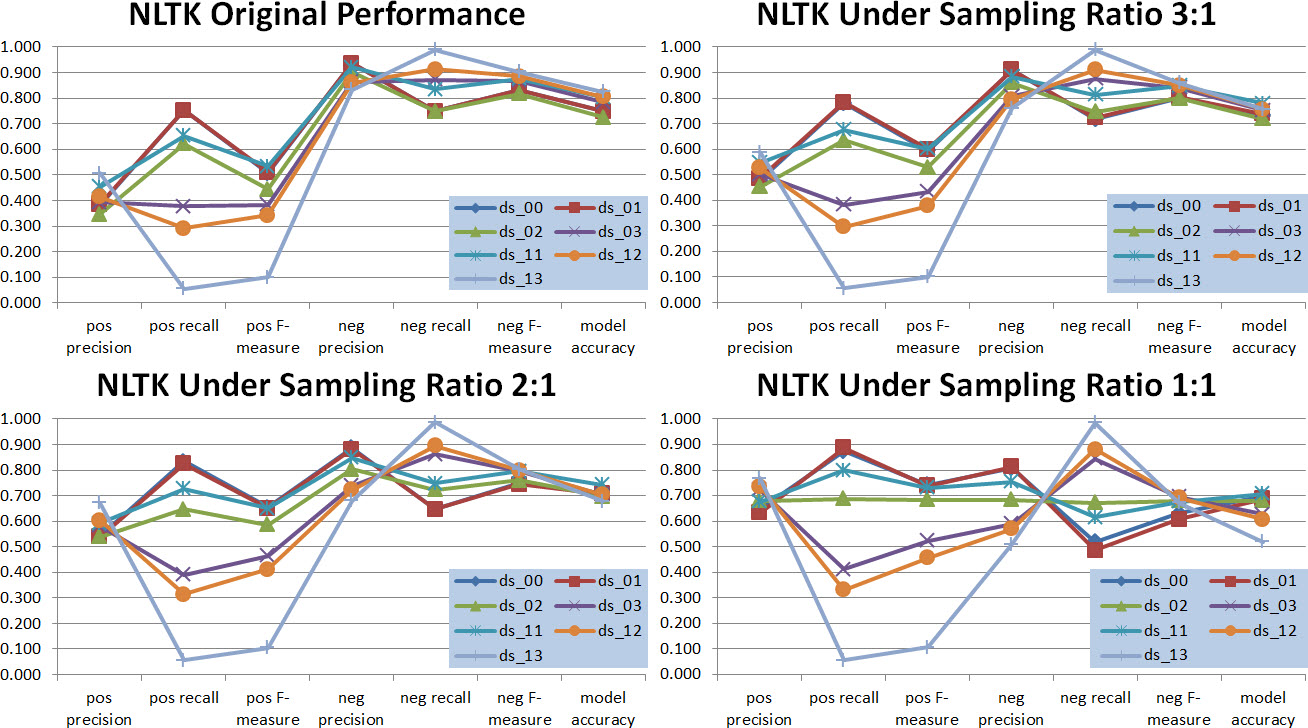
\includegraphics[width=1\textwidth]{Figures/Chapter5/nltk_process_chart_03.jpg}
	\caption[NLTK model performance using under sampling]{Graph showing the performance of the NLTK Naive Bayes model for ratios 3:1, 2:1, 1:1 and the original baseline performance measures}
	\label{fig:nltk_process_chart_03}
\end{figure}

It is clear that the performance of the positive class prediction is increasing as the ratio of samples approaches 1:1. The positive recall values for some of the datasets also show modest improvement, however, the values do not show the same improvement for \verb|dataset_03| tri-grams, \verb|dataset_12| bi-grams no stop words and \verb|dataset_13| tri-grams no stop words. This lack of improvement could be attributed to the uniqueness of the bi-grams and tri-grams in the datasets. It was seen in Section \ref{section:data_exploration} that the average frequency of n-grams in these datasets were very close to 1. Also of note is that as the ratio of classes approaches 1:1 the negative class precision and recall values are decreasing. 

At a ratio of 1:1 the overall performance of \verb|dataset_02|, bi-grams including stop words, could, at this early stage of development, be considered very satisfactory. With performance values in all categories of just under 70\% the model is equally accurate predicting both positive and negative classes. If the ability to solely predict the positive class was the main driving force, than both uni-grams models, with a sample ratio of 1:1, offer a better solution but at the cost of over predicting samples as positive. It must be kept in mind that one of the major drawbacks of under sampling in this manner is the risk of discarding samples that may, in fact, be very representative of the general population.

\subsection{Minority Class Over Sampling}
Over sampling of the positive minority class was explored next. Ratios of 3:1, 2:1 and 1:1 were again simulated, but this time, instead of reducing the number of negative samples in order to achieve these ratios the number of positive samples was increased. In line with all testing to this point the method used to increase the number of positive samples was as simple as possible. The implementation, in Python, is shown in Listing \ref{lst:chapter5.2:snipet_02} where a ratio of 2:1 is created.

\begin{lstlisting}[caption={Adjust the postive to negative class ratio}, label=lst:chapter5.2:snipet_02]
# The questions containing bullying are the positive tests
all_pos_ids = reader.fileids('bullying')
random.shuffle(all_pos_ids)

# Ratio 2:1 required
multi = (len(neg_ids)/2) / len(all_pos_ids)
modul = (len(neg_ids)/2) % len(all_pos_ids)

pos_ids = []

for n in range(multi):
    pos_ids = pos_ids + all_pos_ids

pos_ids = pos_ids + all_pos_ids[:modul]
\end{lstlisting}

When under sampling the negative class was randomly shuffled. This time the positive class is shuffled and the number of times the positive samples need to be replicated, to achieve the desired ratio, is calculated in lines 6 and 7. Taking \verb|dataset_13|, 1049 positive sample and 4915 negative, as an example, the number of times the full set of negative samples need to be replicated is $ ((4915/2) / 1049) = 2$. Then using the modulo operator the number of additional samples required is calculated $ ((4915/2) \% 1049) = 359$. So to create the test dataset two complete copies of the positive samples are required and additional 359 samples. As before, the model was generated five time to ensure that an average performance was achieved. Figure \ref{fig:nltk_process_chart_04} compares the performance results from the models generated using under sampling of the majority class with the models generated using over sampling.

\begin{figure}[htbp]
	\centering
	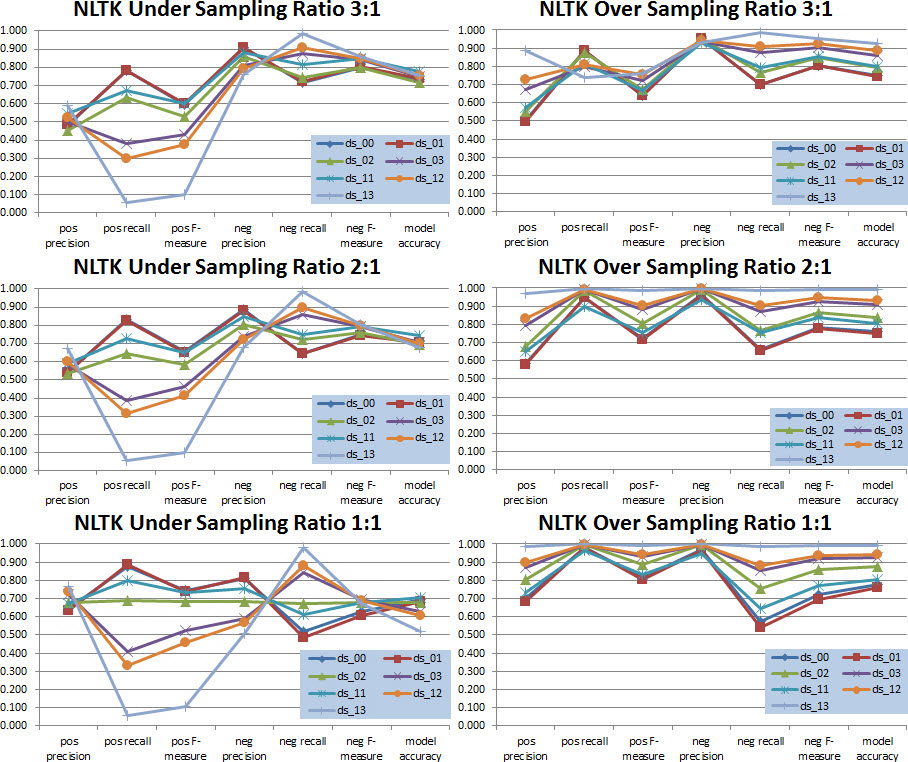
\includegraphics[width=1\textwidth]{Figures/Chapter5/nltk_process_chart_04.jpg}
	\caption[NLTK model performance using over sampling]{Graph showing the performance of the NLTK Naive Bayes model for over sampling ratios of 3:1, 2:1, 1:1 and the original baseline performance measures}
	\label{fig:nltk_process_chart_04}
\end{figure}

It is clear that over sampling of the minority positive class has significantly improved the performance of all models. Bi-gram and tri-gram tokens, with stop words removed, nearly achieving perfection with 99.8\% and 100\% positive sample recall and 88.4\% and 98.4\% negative sample recall respectively. Inversely though, it was also observed that as the ratio of the classes approaches 1:1 that the recall performance of the model predicting the negative class decreased significantly, particularly for all the uni-gram datasets.

Overall though, the results achieved using over sampling of the minority class outperform the models developed using under sampling of the majority class. It must be questioned though whether this gain in performance has been achieved by over fitting the models to the repeated samples? This over fitting to replicated data is a known issue when over sampling is applied.

\subsection{Hybrid Approach}
The third option used to tackle the imbalance of the positive and negative classes was a hybrid approach that uses both under sampling of the majority class and over sampling of the minority class. In this hybrid method, the normal approach is to take the total number of examples and then divide by the number of classes to get the target sample number. For example, in a two class scenario with 800 positive and 400 negative samples, the target number of samples for each class would be 600 if a ratio of 50:50 was the desired ratio. In this section, both classes are over or under sampled to half the total number of examples as just described. However, as the negative class is significantly superior to the negative sample, ratios of 60:40 and 70:30 are also explored. The additional python to achieve the required ratio of samples is shown in Listing \ref{lst:chapter5.2:snipet_03}.

\begin{lstlisting}[caption={Hybrid approach using both over and under sampling}, label=lst:chapter5.2:snipet_03]
# Calculate the number of pos and neg samples
pos_sample = int(float((len(all_neg_ids) + len(all_pos_ids)))
                 * 0.4)
neg_sample = int(float((len(all_neg_ids) + len(all_pos_ids)))
                 * 0.6)
# Ratio 50:50 required
multi_pos = pos_sample / len(all_pos_ids)
modul_pos = pos_sample % len(all_pos_ids)

modul_neg = neg_sample % len(all_neg_ids)
\end{lstlisting}

In this model both the positive file ids and the negative file ids are shuffled, not shown, and Listing \ref{lst:chapter5.2:snipet_03} lines 2 to 4 shows how the total number of positive and negative samples are calculated, in this case to a ratio of 60:40. The same sampling technique using \verb|modul| and \verb|multi|, as used in the over sampling model, is used to generate the sample datasets. As the negative class will never be over sampled only the \verb|modul| value needs to be calculated. Figure \ref{fig:nltk_process_chart_05} shows the result of the model execution using the hybrid sampling ratios.

\begin{figure}[htbp]
	\centering
	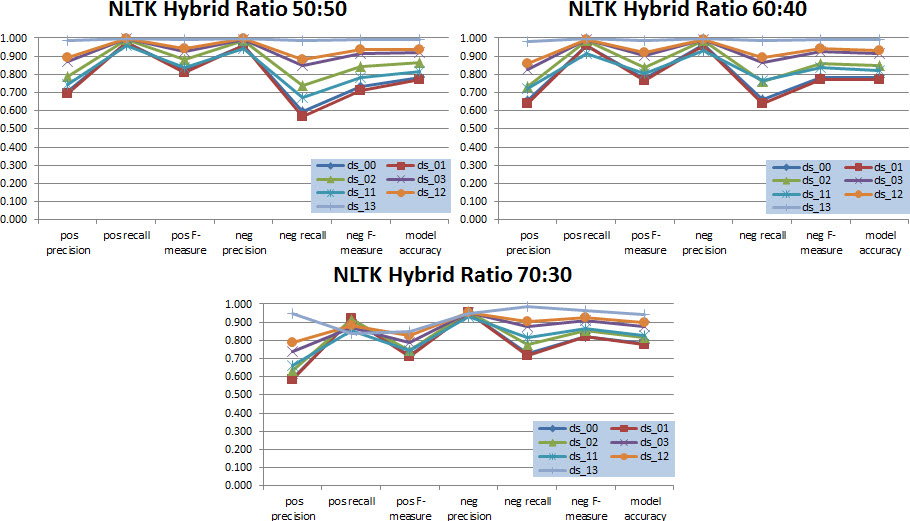
\includegraphics[width=1\textwidth]{Figures/Chapter5/nltk_process_chart_05.jpg}
	\caption[NLTK model performance using hybrid sampling]{Graph showing the performance of the NLTK Naive Bayes model for hybrid sampling ratios of 50:50, 60:40 and 70:30}
	\label{fig:nltk_process_chart_05}
\end{figure}

Comparing Figures \ref{fig:nltk_process_chart_04} and \ref{fig:nltk_process_chart_05} it is clear that the results achieved by over sampling to ratios of 1:1 and 2:1 are very similar to the results achieved by the 50:50 and 60:40 hybrid approach. This fact is highlighted by Table \ref{tab:chapter5:performance_comparison}. The top part of this table gives the results for the over sampling model where a ratio of 1:1 was used. The middle part of the table gives the performance results for the model where hybrid sampling with a ratio of 50:50 was used. The bottom part of the table gives the percentage change between the oversampling model and the hybrid sampling model. Excluding run time measurement, the majority of all performance measures between the two models are within 1\% of each other. Considering all performance measures, again excluding run time, then the total average performance difference between all the models of each type is just 0.18\%. Although the difference between the 2:1 over sampling model and the 60:40 hybrid model is slightly more obvious again the total average difference between the two models is just 1.78\%.

The final thing to consider is the run time. On average, the hybrid model is approximately 35\% faster. This is a significant time saving considering that the performance of the models are so similar. This variance in run time can be explained by the difference in the dataset sizes used. The over sampling dataset had, on average, just over 14,000 samples whereas the hybrid sampling dataset had an average size of just over 8,500. In this direct comparison of two models the obvious choice would be the hybrid approach. This difference in execution time could be pivotal is selecting the best models.

\begin{table}[h]
\centering
\caption[Performance comparison of over sampling and hybrid sampling]{Table giving the performance measured for over sampling at ratio 1:1 and hybrid sampling at 50:50 and the percentage differences}
\label{tab:chapter5:performance_comparison}
\begin{tabular}{rccccccc}
	\toprule
	\multicolumn{4}{c}{\textbf{Over Sampling Ratio 1:1}} \\
	\cmidrule(r){1-4}
     & \textbf{ds\_00}  & \textbf{ds\_01} & \textbf{ds\_02} & \textbf{ds\_03} & \textbf{ds\_11} & \textbf{ds\_12} & \textbf{ds\_13}   \\
    \midrule
	pos precision & 0.698 & 0.682 & 0.804 & 0.872 & 0.733 & 0.896 & 0.984\\
	pos recall & 0.981 & 0.981 & 0.997 & 0.998 & 0.965 & 0.998 & 1.000\\
	pos F-measure & 0.815 & 0.804 & 0.890 & 0.930 & 0.833 & 0.944 & 0.992\\
	neg precision & 0.968 & 0.966 & 0.996 & 0.998 & 0.949 & 0.997 & 1.000\\
	neg recall & 0.574 & 0.542 & 0.756 & 0.853 & 0.647 & 0.884 & 0.984\\
	neg F-measure & 0.720 & 0.693 & 0.859 & 0.919 & 0.769 & 0.937 & 0.992\\
	model accuracy & 0.777 & 0.761 & 0.876 & 0.925 & 0.806 & 0.941 & 0.992\\
	run time & 17.538 & 16.376 & 24.878 & 27.112 & 14.181 & 18.385 & 14.658\\
    \bottomrule
\end{tabular}
\begin{tabular}{rccccccc}
	\multicolumn{4}{c}{\textbf{Hybrid Sampling Ratio 50:50}} \\
	\cmidrule(r){1-4}
     & \textbf{ds\_00}  & \textbf{ds\_01} & \textbf{ds\_02} & \textbf{ds\_03} & \textbf{ds\_11} & \textbf{ds\_12} & \textbf{ds\_13}   \\
	\midrule
	pos precision & 0.707 & 0.692 & 0.791 & 0.870 & 0.744 & 0.894 & 0.984 \\
	pos recall & 0.975 & 0.975 & 0.992 & 0.995 & 0.957 & 0.996 & 1.000 \\
	pos F-measure & 0.819 & 0.809 & 0.880 & 0.928 & 0.837 & 0.942 & 0.992 \\
	neg precision & 0.959 & 0.957 & 0.989 & 0.994 & 0.940 & 0.996 & 1.000 \\
	neg recall & 0.595 & 0.566 & 0.737 & 0.850 & 0.670 & 0.881 & 0.984 \\
	neg F-measure & 0.734 & 0.711 & 0.844 & 0.917 & 0.782 & 0.935 & 0.992 \\
	model accuracy & 0.785 & 0.770 & 0.864 & 0.923 & 0.813 & 0.939 & 0.992 \\
	run time & 11.036 & 10.405 & 16.327 & 18.245 & 9.040 & 11.817 & 9.325 \\
	\bottomrule
\end{tabular}
\begin{tabular}{rccccccc}
	\multicolumn{4}{c}{\textbf{Percentage Difference}} \\
	\cmidrule(r){1-4}
     & \textbf{ds\_00}  & \textbf{ds\_01} & \textbf{ds\_02} & \textbf{ds\_03} & \textbf{ds\_11} & \textbf{ds\_12} & \textbf{ds\_13}   \\
	\midrule
	pos precision & 1.28 & 1.49 & -1.64 & -0.23 & 1.51 & -0.24 & 0 \\
	pos recall & -0.64 & -0.64 & -0.51 & -0.30 & -0.83 & -0.13 & 0 \\
	pos F-measure & 0.49 & 0.61 & -1.14 & -0.26 & 0.49 & -0.19 & 0 \\
	neg precision & -0.89 & -0.90 & -0.69 & -0.34 & -0.93 & -0.15 & 0 \\
	neg recall & 3.71 & 4.47 & -2.55 & -0.26 & 3.51 & -0.31 & 0 \\
	neg F-measure & 2.04 & 2.53 & -1.76 & -0.30 & 1.69 & -0.24 & 0 \\
	model accuracy & 0.96 & 1.18 & -1.39 & -0.28 & 0.91 & -0.21 & 0 \\
	run time & -37.07 & -36.46 & -34.37 & -32.70 & -36.25 & -35.72 & -36.38 \\
	\bottomrule
\end{tabular}
\end{table}

\subsection{Most Frequently Occurring Features}
Where over and under sampling tackles the class imbalance problem by attempting to equalise the number of positive and negative samples, another approach that was explored was to determine if the class imbalance problem could be solved by feature selection. Using a frequency distribution of all positive and negative tokens, the top \textit{x\%} most frequently occurring tokens in each class are chosen. Alternatively, choosing the same top \textit{n} positive and negative samples is also an option.

To achieve this feature sampling required significant changes to the original NLTK Python script described in Section \ref{subsection:nltk-initial_modelling}. A partial listing of the Python Script, where it is different from the original script, is given in Appendix \ref{app:nltk_feature_selection}. The highlights are shown in Listing \ref{lst:chapter5.2:snipet_04} where the additional functionality required to extract to most frequently tokens for the positive class is shown.

The first difference is that the list of all words for the positive class is generated, lines 5 to 8. Next the frequency distribution is created and the top percentage is extracted. In line 12 the top 25\% most frequently occurring tokens are chosen and the comment in line 13 shows how the top 500 tokens would be chosen. Finally, the dictionary describing whether the top features are present or not in the samples is created. As shown in lines 1 to 3 this function is slightly different in that it is checked whether each token is one of the top tokens and, if it is, only then is it included as a feature.

\begin{lstlisting}[caption={Selecting the most frequently occuring tokens}, label=lst:chapter5.2:snipet_04]
def pos_word_feats(words):
    return dict([(word, True) for word in words
                 if word in top_pw])

pos_words = []

for fileid in pos_ids:
    pos_words += [word for word in (reader.words(fileid))]

pw_dist =  nltk.FreqDist(pos_words)

top_pw = pw_dist.keys()[:int(len(pw_dist.keys())*.25)]
# top_pw = pw_dist.keys()[:500]

pos_feat = [(pos_word_feats(reader.words(fileids=[f])),
             'bullying')
            for f in pos_ids]
\end{lstlisting}

The performance measures returned using the most frequently occurring tokens was very disappointing and they did not show any improvement over the baseline from Section \ref{subsection:nltk-initial_modelling}. Feature selection combined with over, under and hybrid sampling actually returned worse performance measures than the sampling techniques did on their own.  
\section{Scikit-learn Modelling}
\label{subsection:scikit-learn}

The Natural Language Toolkit produced some promising models and was quite easy to use. It did not, however, offer much choice or scope for different lines of investigation during model development. Although additional functionality is made available to the developer through a wrapper for Scikit-Learn \cite{scikit-learn}, in this section the NLTK is left behind and focus, instead, turns to the use of Scikit-Learn. Initially, some simple models are quickly developed and explored before attention is given to the more advanced fine tuning operations that are available.

\subsection{Model Development}
Whilst the development of the Scikit-Learn model follows a very similar flow to that utilised for the NLTK model, Scikit-Learn could be considered as a much more advanced toolkit where built-in methods provide a lot of the required data manipulation functionality. As well as this data manipulation functionality Scikit-Learn also provides a better selection of learner algorithms. For the initial investigation, a Naive Bayes and a Support Vertor Machine learner were considered.

The first step in the process is to access the data. Whilst the data could have been accessed directly from the NLTK corpora location, it was decided to pre-process the dataset such that each corpus was consolidated into a single comma separated file with two attributes. The first attribute was the class where \verb|0| was used to represent a bullying sample and \verb|1| not bullying sample. The second attribute was the text of the question. For example:

\verb|    1,"your really cute"| \\
\verb|    0,"could you just like not breathe"|

A comma separated versions reader was then used to load the data. The class attribute was loaded into an array call target, class is a reserved word in Python, and the text of the question was loaded into an array named data.

Previously, when using the NLTK, the models developed were not evaluated using unseen data. However, as the performance of the models developed using Scikit-Learn will be evaluated against unseen data, the next step was to separate the data into a training dataset and a testing dataset. Rather than having to manually split the data, and ensure that the division is representative, Scikit-Learn provides a \verb|cross_validation.train_test_split| operator that will automatically split the dataset into random training and testing subsets. The code snippet in Listing \ref{lst:chapter5.3:snipet_01} shows how this function is used.

\begin{lstlisting}[caption={Using the cross validation train test split function}, label=lst:chapter5.3:snipet_01]
X_train, X_test, y_train, y_test = \
     cross_validation.train_test_split(
         data, target, test_size=0.2,
         random_state=(random.randrange(1,100)))
\end{lstlisting}

The data and target arrays are the first two parameters passed. The third parameter passed is the proportion of the dataset to include in the test set. In this case 20\% of the data will be held back for the test dataset. The final parameter is the pseudo-random number generator state used for random sampling. A random number in the range 1 to 100 is used for each invocation. By convention the returned arrays are named \verb|X_train, X_test, y_train, y_test| where \verb|X_train, X_test| are the datasets representing the split data array and \verb|y_train, y_test| are the datasets representing the split target array.

The next step is to create an instance of a \verb|TfidfVectorizer| which performs two main tasks. The first is to convert a collection of text documents, in this case the array of training questions, into a matrix that is a sparse representation of token counts. The second tasks transforms the count matrix into a term frequency inverse document frequency (TF-IDF) representation. There are many options that can be specified when creating the \verb|td-idf| object which will be explored later. Whereas the training data is transformed into a document / token matrix and the TD-IDF of each token is calculated, the test data is only transformed into the sparse matrix format for use later.

\begin{lstlisting}[caption={Create TfidfVectorizer and transform training and test data}, label=lst:chapter5.3:snipet_02]
tfidf   = TfidfVectorizer()
X_train = tfidf.fit_transform(X_train)
X_test  = tfidf.transform(X_test)
\end{lstlisting}

The final step, before evaluating the model, is to fit the model to the training data and then predict the class of testing data. Listing \ref{lst:chapter5.3:snipet_03} shows the creation of a Multinomial Naive Bayes model and its fitting to the training data, followed by the class prediction for the training dataset. Also shown in brackets is the generation of the second model that will be examined, the Linear Support Vector Classifier. As well as the performance measurements generated for the NLTK models scikit-learn also gives the resulting confusion matrix.

\begin{lstlisting}[caption={Create TfidfVectorizer and transform training and test data}, label=lst:chapter5.3:snipet_03]
model = MultinomialNB().fit(X_train, y_train)
# model = LinearSVC().fit(X_train, y_train)

y_pred = model.predict(X_test)
\end{lstlisting}

The complete listing for this simple Scikit-Learn learner is given in Appendix \ref{app:simple_scikit}.

\subsection{Model Execution and Performance}

Once developed, the model was executed for each of the seven datasets previously defined. It was also run for the Multinomial Naive Bayes learner and the Linear Support Vector learner using the default parameters (in both cases passing no parameters uses all default parameters options). Figure \ref{fig:scikit_process_chart_01} shows the performance of these two models.

\begin{figure}[htbp]
	\centering
	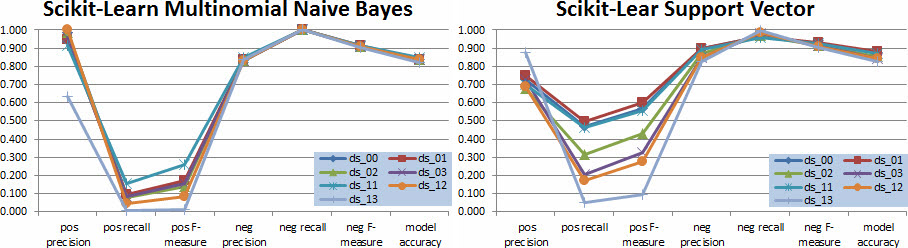
\includegraphics[width=1\textwidth]{Figures/Chapter5/scikit_process_chart_01.jpg}
	\caption[Scikit-Learn model performance using default parameters]{Graph showing the performance of the Scikit-Learn Multinomial Naive Bayes and Linear Support Vector learners using the default parameters}
	\label{fig:scikit_process_chart_01}
\end{figure}
 
It is immediately apparent that neither learner has performed well when predicting the positive class, but it is clear that the Naive Bayes classifier has performed particularly badly. Both models returned good results predicting the negative class with the Support Vector classifier performing the better of the two. However, with the use of Scikit-Learn it is also possible to dig deeper into these performances by analysing the confusion matrices for each of the datasets and models. Table \ref{tab:chapter5:nb_confusion_01} and Table \ref{tab:chapter5:sv_confusion_01} both give sample matrices, and it can be seen that the Naive Bayes model nearly exclusively predicted all samples as negative and although the Support Vector model managed to achieve better results it still favoured the negative class. The extreme examples are the performance of the models on dataset 13. In total, the Support Vector model only predicted 17 positive samples and the Naive Bayes model only predicted 3 positive samples or less than 1.5\% of the total possible number. It was assumed that the first simple NLTK models were also only predicting negative classes so Scikit-Learn providing this extra information is an advantage.

As five-fold cross validation was used this meant that five confusion matrices, one for each execution, were generated. It should be noted that the confusion matrices show in Tables \ref{tab:chapter5:nb_confusion_01} and Table \ref{tab:chapter5:sv_confusion_01} are actual numbers from one of the models and not averages as calculating averages would not make any sense.

\begin{table}[h]
	\centering
	\caption[Confusion matrices from the initial Scikit-Learn Naive Bayes model]{Table giving summary confusion matrix results for each test dataset from the initial Scikit-Learn Naive Bayes model}
	\label{tab:chapter5:nb_confusion_01}
	\begin{tabular}{lrrrrrrr}
		\toprule
		& \textbf{ds\_00}  & \textbf{ds\_01} & \textbf{ds\_02} & \textbf{ds\_03} & \textbf{ds\_11} & \textbf{ds\_12} & \textbf{ds\_13}   \\
		\midrule
		Pos Samples & 335 & 328 & 320 & 309 & 352 & 276 & 211 \\
		Neg Samples & 1580 & 1581 & 1466 & 1327 & 1536 & 1333 & 982 \\
		\midrule
		Pred Pos True Pos & 35 & 34 & 30 & 28 & 59 & 21 & 2 \\
		Pred Pos True Neg & 0 & 5 & 0 & 0 & 7 & 0 & 1 \\
		Pred Neg True Neg & 1580 & 1576 & 1466 & 1327 & 1529 & 1333 & 981 \\
		Pred Neg True Pos & 310 & 294 & 290 & 281 & 293 & 255 & 209 \\
		
		\bottomrule
    \end{tabular}
\end{table}

\begin{table}[h]
	\centering
	\caption[Confusion matrices from the initial Scikit Support Vector model]{Table giving summary confusion matrix results for each test dataset from the initial Scikit Support Vector model}
	\label{tab:chapter5:sv_confusion_01}
	\begin{tabular}{lrrrrrrr}
		\toprule
		& \textbf{ds\_00}  & \textbf{ds\_01} & \textbf{ds\_02} & \textbf{ds\_03} & \textbf{ds\_11} & \textbf{ds\_12} & \textbf{ds\_13}   \\
		\midrule
		Pos Samples & 353 & 335 & 306 & 295 & 361 & 292 & 212 \\
		Neg Samples & 1562 & 1574 & 1471 & 1341 & 1527 & 1317 & 981 \\
		\midrule
		Pred Pos True Pos & 172 & 173 & 104 & 64 & 163 & 61 & 12 \\
		Pred Pos True Neg & 67 & 49 & 66 & 22 & 56 & 19 & 5 \\
		Pred Neg True Neg & 1495 & 1525 & 1405 & 1319 & 1471 & 1298 & 976 \\
		Pred Neg True Pos & 181 & 162 & 202 & 231 & 198 & 231 & 200 \\
		
		\bottomrule
    \end{tabular}
\end{table}

A very interesting performance measure, that has only been briefly mentioned thus far, is the length of time each model takes to run. An examination of the run times for the first NLTK model and these first Scikit-Learn models showed that the Scikit-Learn models were between 87.5\% and 90.5\% faster with executions times around 1 second compared to 10 seconds for the NLTK models. This is a significant discovery. Given a choice between two models that have similar performance measurements, but one is ten times faster, the model chosen would always be the faster model. Hopefully this runtime advantage is maintained as more complexity is added to the Scikit-Learn models and the other performance measures are on a par with or better than the NLTK models. The time comparisons are shown in Figure \ref{fig:runtime_comp}.

\begin{figure}[htbp]
	\centering
	\includegraphics[width=.75\textwidth]{Figures/Chapter5/runtime_comp.jpg}
	\caption[NLTK - Scikit-Learn runtime comparison]{Graph showing the difference in runtime performance between the NLTK and Scikit-Learn}
	\label{fig:runtime_comp}
\end{figure}

\subsection{Further Exploration}
As with the NLTK model it is important to now examine some of the additional options offered by the Scikit-Learn TF-IDF implementation and also the Naive Bayes and Support Vector classifiers to determine if the model performance can be further improved before addressing the class imbalance. First the TF-IDF implementation will be examined.

The \verb|TfidfVectorizer| object performs two main tasks. The first is to convert a collection of text documents, in this case the array of training questions, into a matrix that is a sparse representation of token counts. It then transforms this count matrix into a term frequency inverse document frequency (TF-IDF) representation. In all, there are over twenty parameters that can be used to customise and fine tune the performance of this operator but for this research project only the following will be examined \cite{scikit-learn}:

\begin{enumerate}

	\item \textbf{ngram\_range}: tuple (min\_n, max\_n) \\
	The lower and upper boundary of the range of n-values for different n-grams to be extracted. All values of n such that $min_n <= n <= max_n$ are used.
	
	\item \textbf{stop\_words}: string {'english'}, list, or None (default) \\
	\verb|english| is currently the only supported string value and this has the affect of removing English stop words.
	
	\item \textbf{max\_df}: float in range [0.0, 1.0] or int, optional, 1.0 by default \\
	When building the vocabulary ignore terms that have a term frequency strictly higher than the given threshold.
	
	\item \textbf{norm}: 'l1', 'l2' or None, optional \\
	Norm used to normalize term vectors where \verb|l1| is the Manhattan Norm, $\lVert{x}\rVert = \sum_i \lvert x_i \rvert$, and \verb|l2| is the Euclidean Norm, $\lVert{x}\rVert = \sqrt{\sum_i \lvert x_i^2 \rvert}$. None is for no normalization.
	

\end{enumerate}

Other parameters allow preprocessing of the corpus, similar to that described in Chapter \ref{chapter4}, and more advanced control of the TF-IDF calculation, but these were not considered.

In total six models of interest were examined, all of which were based on \verb|dataset_01|, uni-grams without stop words removed. Three were based on the Naive Bayes classifier and three on the Support Vector classifier. The first model of each classifier type used the \verb|stop_words| parameter to remove frequently occurring tokens and these execution runs were called \verb|run_01| and \verb|run_04|. The second and third iteration of each model used the \verb|ngram_range| parameter to specify the use of bi-grams,\verb|run_02| and \verb|run_03|, and tri-grams \verb|run_05| and \verb|run_06|. What is different with the Scikit-Learn N-Gram parameter, when compared with the NLTK version, is that the Scikit-Learn retains all the n-grams in the range specified. For example, when \verb|ngram_range(1, 3)| is specified, this means that all uni-grams, bi-grams and tri-grams will be returned. The performance results from the execution of these six models is shown in Figure \ref{fig:scikit_process_chart_02}.

\begin{figure}[htbp]
	\centering
	\includegraphics[width=.6\textwidth]{Figures/Chapter5/scikit_process_chart_02.jpg}
	\caption[Scikit-Learn model performance with default parameters]{Graph showing the performance of the Scikit-Learn Multinomial Naive Bayes and Linear Support Vector learners using the default parameters}
	\label{fig:scikit_process_chart_02}
\end{figure}

Comparing Figures \ref{fig:scikit_process_chart_01} and \ref{fig:scikit_process_chart_02}, and from an analysis of the details of the results, it is clear that there was an overall improvement in the models. Though this improvement was especially seen in the models that utilised bi-grams and tri-grams, models \verb|run_02, 03, 05 & 06|, the improvement was attributed to the inclusion of uni-grams. This fact was borne out by testing these models again without including uni-grams, \verb|ngram_range(2, 3)|. This yielded similarly disappointing performance results to the models utilising the original bi-grams and tri-grams only datasets. The inclusion or the \verb|norm| parameter did show a very slight improvement of less than 1\% in the performance of the models but the \verb|max_df| appeared to have little or no affect at all. The \verb|TfidfVectorizer| is now as shown in Listing \ref{lst:chapter5.3:snipet_04}.

\begin{lstlisting}[caption={TfidfVectorizer parameters}, label=lst:chapter5.3:snipet_04]
tfidf = TfidfVectorizer(
      stop_words='english'
    , ngram_range=(1, 3)
    , norm='l2'
)
\end{lstlisting}

Looking next at the Multinomial Naive Bayes classifier the only obvious parameter to consider at this stage is the \verb|alpha| parameter which is an additive Laplace smoothing parameter. Values of \verb|alpha| of 0.1, 0.01, 0.001 and 0.0001 were tested. Although all values returned improved results when compared with the default value of 1 it appeared that 0.001 gave slightly better results than the others. The performance measures returned when the value of \verb|alpha| was set to 0.001 is also shown in Figure \ref{fig:scikit_process_chart_02} as \verb|run_07|. It is clearly seen that introducing the \verb|alpha| parameter has significantly improved the predictive performance of the Naive Bayes classifier bringing its results in line with the Support Vector learner. Whilst there are Support Vector parameters that could be modified to possibly improve the performance of the model they are more associated with addressing class imbalance so they have been left to the next section where this topic is addressed.

It should be pointed out at this stage that the analysis of the parameters in this section is very much based on observation and manual analysis of the performance results returned. In the next section, a more scientific grid based approach will be used in order to fine tune the parameter values.


\section{Scikit-learn - Class Imbalance}
\label{subsection:scikit-class-imbalance}

In this section, similar to NLTK, the class imbalance issue is tackled and will use the same under sampling of the majority class, over sampling of the minority class and hybrid sampling techniques that were initially explored in Section \ref{subsection:nltk-class_imbalance}.

However, before addressing the class imbalance, two other very useful features of Scikit-Learn, the pipeline and grid based searches, are utilised to fine turn the classifiers from the previous section.

\subsection{Pipeline and Grid Search}

The Scikit-Learn \verb|Pipeline| class, when used in conjunction with the \verb|GridSearchCV| class, can be used to assemble several transformation and estimator steps that can be executed together in sequence while setting different parameters for each transformer or estimator. In this tentative examining of these features the transformer that will be examined is the TF-IDF transformer and the estimators, or classifier, will be the Multinomial Naive Bayes. Later, when looking at cost based estimation, the Linear Support Vector classifier will also be examined. 

When using a grid search, an initial range of values for a set of parameters are defined that are then exhaustively examined such that all possible combinations of parameter values are tested. Where parameters are numeric the initial range of values are typically well spread out and then fine tuned over a number of searches until the optimal value is found. When applied to the Multinomial Naive Bayes estimator with the TF-IDF transformer, the initial parameter ranges applied were as shown in Listing \ref{lst:chapter5.4:snipet_01}. The data is then fitted and the best score achieved that can be obtained, as well as the parameter values that yielded the best score, are returned. Some knowledge of the transformers and estimator used in the grid search is assumed as blindly setting arbitrary values for random parameters could give unexpected results that on the surface appear good but on closer examination do not yield the desired results. When used with the Multinomial Naive Bayes estimator the default scoring value is the overall accuracy of the model. The scoring value could be set to score on recall or precision, but this could return a perfect recall score where all samples are given the same class. This would not be the desired result.

\begin{lstlisting}[caption={Using grid search to fine tune parameter values}, label=lst:chapter5.4:snipet_01]
# Create a pipeline with a transformer and a estimator
pipeline = Pipeline([
    ('tfidf', TfidfVectorizer()),
    ('clf',   MultinomialNB()),
])

# Define the parameter ranges
parameters = {
    'tfidf__stop_words': [None, 'english'],
    'tfidf__ngram_range': [(1, 1),
                           (1, 2),
                           (1, 3),
                           (2, 2),
                           (2, 3),
                           (3, 3)],
    'tfidf__norm': ['l1', 'l2'],
    'clf__alpha': [10, 1.0, 0.1, 0.01],
}
\end{lstlisting}

The results returned from the first running of the grid search object were:

\begin{spverbatim}
Done in 163.616s
Best score: 0.873
Best Parameters:
    clf__alpha:         0.1
    tfidf__ngram_range: (1, 3)
    tfidf__norm:        'l2'
    tfidf__stop_words:  None
\end{spverbatim}
 
Although further fine tuning of the \verb|alpha| parameter was performed, no further gains were made. When these parameter values were fed back into the Scikit-Learn Python script as it existed at the end of the previous section it can be seen, as shown in Figure \ref{fig:scikit_process_chart_03} and Table \ref{tab:chapter5:grid_search_01}, that whilst the overall accuracy of the model has indeed improved, this improvement was mostly achieved by a significant improvement in the precision of the positive class at the cost of a small reduction in the positive class recall. It could be argued, depending on the final production use of the model, that this reduction in positive class recall is an acceptable sacrifice given that the maximum model accuracy has been achieved. Balancing this trade off between gains in one area over losses in another will, in the final model, be determined by whether it is more important to correctly predict the most amount of bullying samples as bullying, a high recall value, while accepting that a significant proportion of not bullying sample will incorrectly be classified as bullying or is it better to maximise the precision of each class.

In Figure \ref{fig:scikit_process_chart_03} and Table \ref{tab:chapter5:grid_search_01} \verb|run_01| represents the previous manually tuned parameters and \verb|run_02| the results obtained using the parameters from the grid search.

\begin{figure}[htbp]
	\centering
	\includegraphics[width=0.6\textwidth]{Figures/Chapter5/scikit_process_chart_03.jpg}
	\caption[Scikit-Learn comparing best manual results with grid search results]{Graph showing a comparison of the results from the best manually tuned parameters against the best grid search parameters for a Multinomial Naive Bayes classifier}
	\label{fig:scikit_process_chart_03}
\end{figure}

\begin{table}[h]
	\centering
	\caption[Grid search performance and confusion matrix comparison]{Table showing a comparison of the results from best manually tuned parameters against the best grid search parameters for a Multinomial Naive Bayes classifier}
	\label{tab:chapter5:grid_search_01}
	\begin{tabular}{lrr}
		\toprule
		\textbf{Performance}& \textbf{run\_01}  & \textbf{run\_02}   \\
		\midrule
		pos precision & 0.648 & 0.816  \\
		pos recall & 0.456 & 0.342  \\
		pos F-measure & 0.534 & 0.480  \\
		neg precision & 0.898 & 0.882  \\
		neg recall & 0.950 & 0.984  \\
		neg F-measure & 0.922 & 0.930  \\
		model accuracy & 0.868 & 0.875  \\
		run time & 2.370 & 3.519  \\
		\midrule
		\textbf{Confusion} &  &   \\
		\textbf{Martix} & \textbf{run\_01} & \textbf{run\_02}  \\
		\midrule
		pos samples & 344 & 345  \\
		neg samples & 1565 & 1564  \\
		Pred Pos True Pos & 157 & 117  \\
		Pred Pos True Neg & 77 & 21  \\
		Pred Neg True Neg & 1488 & 1543  \\
		Pred Neg True Pos & 187 & 228  \\		
		\bottomrule
    \end{tabular}
\end{table}

From this point on, as class imbalance options are investigated, the pipeline and grid search classes will continue to be used. The approach is to run the pipeline grid search on the various datasets and then use the parameters returned to get the complete set of performance measures from the model.

A sample Python grid search script is given in Appendix \ref{app:grid_scikit}.

\subsection{Class Sampling}
In this section, the sampling logic previously used with the NLTK models are now applied to the pipeline grid search using Scikit-Learn Multinomial Naive Bayes and Linear Support Vector classifiers with a TF-IDF transformer. Datasets with ratios of 3:1, 2:1 and 1:1, are generated for under sampling of the majority class and over sampling of the minority class and for the hybrid approach the negative class and positive class are sampled to ratios of 70:30, 60:40 and 50:50 respectively. The results from these model executions are shown in Figure \ref{fig:scikit_process_chart_04}. 

\begin{figure}[htbp]
	\centering
	\includegraphics[width=1.0\textwidth]{Figures/Chapter5/scikit_process_chart_04.jpg}
	\caption[Scikit-Learn sampling with grid search results]{Graphs showing the performance results for grid searches using under, over and hybrid sampling with Multinomial Naive Bayes and Linear Support Vector classifiers}
	\label{fig:scikit_process_chart_04}
\end{figure}

In Figure \ref{fig:scikit_process_chart_04} \verb|run_01, 02 & 03| are the results from the Multinomial Naive Bayes classifier and reflect ratios \verb|3:1, 2:1 1:1 or 70:30, 60:40 & 50:50| respectively while \verb|run_04, 05 & 06| are the results from the Linear Support Vector classifier and are representative of the same sample ratios. With just a cursory look at these charts, it is quite clear that over sampling of the minority class and hybrid sampling both significantly out perform under sampling of the majority class. Because of these results, under sampling will not be analysed further. The actual performance values achieved for over sampling and hybrid sampling are given in Table \ref{tab:chapter5:grid_search_performance_comparison}.


\begin{table}[h]
\centering
\caption[Performance comparison of over sampling and hybrid sampling]{Table comparing the grid search performance of over sampling and hybrid sampling using Multinomial Naive Bayes and Linear Support Vector classifiers}
\label{tab:chapter5:grid_search_performance_comparison}

\begin{tabular}{rccccccc}
	\toprule
	\multicolumn{4}{c}{\textbf{Over Sampling}} \\
	\cmidrule(r){1-4}
	 & \textbf{run\_01} & \textbf{run\_02} & \textbf{run\_03} & \textbf{run\_04} & \textbf{run\_05} & \textbf{run\_06} \\
	\midrule
	pos precision & 0.874 & 0.920 & 0.864 & 0.832 & 0.868 & 0.912 \\
	pos recall & 0.776 & 0.914 & 0.994 & 0.826 & 0.952 & 1.000 \\
	pos F-measure & 0.822 & 0.916 & 0.926 & 0.830 & 0.908 & 0.954 \\
	neg precision & 0.928 & 0.958 & 0.992 & 0.942 & 0.974 & 1.000 \\
	neg recall & 0.962 & 0.958 & 0.846 & 0.942 & 0.928 & 0.904 \\
	neg F-measure & 0.944 & 0.958 & 0.916 & 0.942 & 0.948 & 0.950 \\
	model accuracy & 0.916 & 0.945 & 0.919 & 0.915 & 0.935 & 0.952 \\
	run time & 4.056 & 4.765 & 6.871 & 5.274 & 6.312 & 4.017 \\
	\bottomrule
\end{tabular}

\begin{tabular}{rccccccc}
	\multicolumn{4}{c}{\textbf{Hybrid Sampling}} \\
	\cmidrule(r){1-4}
	 & \textbf{run\_01} & \textbf{run\_02} & \textbf{run\_03} & \textbf{run\_04} & \textbf{run\_}05 & \textbf{run\_06} \\
    \midrule
	pos precision & 0.904 & 0.894 & 0.830 & 0.830 & 0.854 & 0.890 \\
	pos recall & 0.812 & 0.922 & 0.978 & 0.866 & 0.948 & 0.964 \\
	pos F-measure & 0.856 & 0.908 & 0.898 & 0.848 & 0.898 & 0.926 \\
	neg precision & 0.924 & 0.948 & 0.978 & 0.940 & 0.964 & 0.962 \\
	neg recall & 0.964 & 0.926 & 0.798 & 0.924 & 0.892 & 0.880 \\
	neg F-measure & 0.942 & 0.936 & 0.878 & 0.930 & 0.926 & 0.920 \\
	model accuracy & 0.917 & 0.925 & 0.889 & 0.904 & 0.915 & 0.924 \\
	run time & 3.784 & 3.521 & 3.579 & 3.964 & 2.467 & 2.374 \\
    \bottomrule
\end{tabular}

\begin{tabular}{rccccccc}
	\multicolumn{4}{c}{\textbf{Percentage Difference}} \\
	\cmidrule(r){1-4}
	 & \textbf{run\_01} & \textbf{run\_02} & \textbf{run\_03} & \textbf{run\_04} & \textbf{run\_05} & \textbf{run\_06} \\
	\midrule
	pos precision & 3.43\% & -2.83\% & -3.94\% & -0.24\% & -1.61\% & -2.41\% \\
	pos recall & 4.64\% & 0.88\% & -1.61\% & 4.84\% & -0.42\% & -3.60\% \\
	pos F-measure & 4.14\% & -0.87\% & -3.02\% & 2.17\% & -1.10\% & -2.94\% \\
	neg precision & -0.43\% & -1.04\% & -1.41\% & -0.21\% & -1.03\% & -3.80\% \\
	neg recall & 0.21\% & -3.34\% & -5.67\% & -1.91\% & -3.88\% & -2.65\% \\
	neg F-measure & -0.21\% & -2.30\% & -4.15\% & -1.27\% & -2.32\% & -3.16\% \\
	model accuracy & 0.14\% & -2.14\% & -3.28\% & -1.15\% & -2.08\% & -2.93\% \\
	run time & -6.71\% & -26.11\% & -47.91\% & -24.84\% & -60.92\% & -40.90\% \\
	\bottomrule
\end{tabular}
\end{table}

When analysing each models performance results, the nature of the research in hand, and its objectives, are the steering force giving guidance to determine which model best meets the criteria. The main objective of this research is to identify bullying questions such that they could potentially be flagged either before posting or before being read. The perfect solution would be one where all questions identified as bullying, the positive class, and all not bullying questions, the negative class, are correctly identified all of the time. Failing this, because of the potential harm that could be caused by a vulnerable teen reading a bullying question, the most important criterion is that as many bullying questions as possible are identified. This implies that maximising positive class recall is the number one criteria when classifying samples. However, simply over predicting samples as bullying would not be an acceptable solution. Consider an analogy to spam detection in emails. If ham emails are continuously quarantined because they are incorrectly labelled as spam, confidence in the filter would quickly be lost leading to it being un-installed. So the second criterion, when evaluating these models, is to also maximise negative class recall.

It is worth remembering the performance measurements achieved are the average results from five-fold cross validation where 80\% of the samples were used to train the model and 20\% used for testing. Examining first the over sampling models, the top three positive recall values are from the linear support vector model with ratio of 1:1, the Naive Bayes model with ratio 1:1 and linear support vector model with ratio 2:1. Although positive recall for the first two models are 100\% and 99.4\% respectively, the negative recall for the linear support vector 2:1 ratio model is actually the highest. Given the known risk of over fitting when over sampling is used, and the possible inability of the model to generalise to the entire population, the most likely best candidate model from the over sampling experiments would be \verb|run_05|. This is the linear support vector classifier using a negative to positive sample ratio of 2:1 and a n-gram seting of (1, 3). The results from the hybrid experiments were very similar with both classifiers using 50:50 sample ratios having the best positive recall. Once again \verb|run_05| with the middle sample ratio, in this case 60:40 negative to positive, and the Linear SV classifier with a (1, 2) n-gram parameter had probably the best overall balanced performance. Comparing the top two models in each sampling experiment directly there is very little difference in the positive recall values with over sampling having the edge by just over 0.5\% though the advantage was wider at 2.5\% on negative recall. However, given that hybrid sampling was nearly 61\% faster, as a smaller dataset was used, it would be difficult to choose between the two without performing some more detailed testing.

Also of note, and important to highlight, was the different parameter values returned from the grid search for each model execution, shown in Table \ref{tab:chapter5:grid_search_parameters}. It is no surprise that the most popular n-gram range scheme, especially with over sampling and hybrid sampling, is the (1, 3) scheme which includes uni-grams, bi-grams and tri-grams. The inclusion of all n-grams, coupled with the fact that all but one model also included stop words, must have aided greatly in the identification of each class. L2 was also the most popular normalisation parameter setting with five out of every six models using this setting.   

\begin{table}[h]
\centering
\caption[Sampling parameter values returned by grid search]{Table showing the parameter values returned for each sampling technique by a grid search}
\label{tab:chapter5:grid_search_parameters}

\begin{tabular}{rccccccc}
	\toprule
	\multicolumn{4}{c}{\textbf{Under Sampling Parameters}} \\
	\cmidrule(r){1-4}
	 & \textbf{run\_01} & \textbf{run\_02} & \textbf{run\_03} & \textbf{run\_04} & \textbf{run\_05} & \textbf{run\_06} \\
	\midrule
	tfidf\_\_ngram\_range: & (1, 2) & (1, 2) & (1, 1) & (1, 3) & (1, 1) & (1, 2) \\
	tfidf\_\_norm & l2 & l2 & l1 & l2 & l2 & l2 \\
	tfidf\_\_stop\_words & None & None & None & None & None & None \\
	clf\_\_alpha & 0.1 & 0.2 & 0.2 &  &  &  \\
	\bottomrule
\end{tabular}

\begin{tabular}{rccccccc}
	\multicolumn{4}{c}{\textbf{Over Sampling Parameters}} \\
	\cmidrule(r){1-4}
	 & \textbf{run\_01} & \textbf{run\_02} & \textbf{run\_03} & \textbf{run\_04} & \textbf{run\_}05 & \textbf{run\_06} \\
    \midrule
	tfidf\_\_ngram\_range & (1, 3) & (1, 3) & (1, 3) & (1, 3) & (1, 3) & (1, 2) \\
	tfidf\_\_norm & l2 & l2 & l1 & l2 & l2 & l2 \\
	tfidf\_\_stop\_words & None & None & None & None & None & None \\
	clf\_\_alpha & 0.1 & 0.3 & 0.08 &  &  &  \\    \bottomrule
\end{tabular}

\begin{tabular}{rccccccc}
	\multicolumn{4}{c}{\textbf{Hybrid Sampling Parameters}} \\
	\cmidrule(r){1-4}
	 & \textbf{run\_01} & \textbf{run\_02} & \textbf{run\_03} & \textbf{run\_04} & \textbf{run\_05} & \textbf{run\_06} \\
	\midrule
	tfidf\_\_ngram\_range & (1, 3) & (1, 3) & (1, 3) & (1, 3) & (1, 2) & (1, 3) \\
	tfidf\_\_norm & l2 & l2 & l1 & l2 & l2 & l2 \\
	tfidf\_\_stop\_words & None & None & None & None & None & english \\
	clf\_\_alpha & 0.2 & 0.4 & 0.0075 &  &  &  \\	\bottomrule
\end{tabular}
\end{table}

A sample Python script showing how over sampling was implemented is given in Appendix \ref{app:over_scikit}.


\section{Scikit-learn - Cost Sensitive Learning}
\label{subsection:scikit-learn-cost}

Having looked at under, over and hybrid sampling methods attention now turns towards a cost sensitive learning approach. Cost sensitive learning is considered an algorithmic solution to class imbalance where there is a cost involved in predicting either a false positive or false negative, with no cost for predicting a true positive or true negative. False positives and false negatives can also be treated, costed, differently as well. Consider a cancer diagnoses, for example. It is better to predict a false positive and have the patient undergo further testing to discover they are free from cancer rather than predict a false negative where the patient receives no further tests or treatment which could have grave implications.

Unfortunately, Scikit-Learn does not have a true cost sensitive implementation analogous to the MetaCost algorithm implemented in Weka though some classifiers do offer \verb|class_weight| and \verb|C| parameters, which are optimized implementations of over sampling and under sampling \cite{scikit-learn}. 

\begin{enumerate}

	\item \textbf{C}: float, optional (default=1.0) \\
	Parameter that tells the learner how much to avoid misclassifying each training example. Larger values of \verb|C| will cause a smaller margin hyperplane to be chosen while a small value will increase the size of the hyperplane thus increasing the risk of misclassification.
	
	\item \textbf{class\_weight}: \{dict, ‘auto’\}, optional \\
	Set the parameter C of class i to class\_weight[i]*C for SVC. If not given, all classes are supposed to have weight one. The ‘auto’ mode uses the values of y to automatically adjust weights inversely proportional to class frequencies.
	
\end{enumerate}

It was hoped to evaluate the C Support Vector Classification learner in addition to the Linear Support Vector classifier already examined. However, the results returned were either disappointing or the learner proved impossible to fine tune either returning all positive or all negative predictions when training. 
\section{Choosing the Best Classifiers}
\label{subsection:best-classifiers}

Having completed all NLTK and Scikit-Learn modelling, the next task was to identify which models performed the best to be further evaluated using simulation and which models, even though their performance measures are good, are to be discarded. As previously discussed, the criteria to determine the best model was that it should first maximise recall for the positive bullying class and secondly that it must also maximise recall for the negative not bullying class. As discovered in the literature review in Section \ref{section:3.3}, \citet{kubat_addressing_1997} referred to this measure as the geometric mean of the accuracies measured separately on each class or as $g =\sqrt{\frac{TP}{TP + FN} \cdot \frac{TN}{TN + FP}}$, from now on referred to as the \textit{g-performance}. This measure is essentially the square root of the positive class recall multiplied by the negative class recall. The top classifiers will be further evaluated in the next section by way of a simulation of live data.

\subsection{G-Performance}

The measure used to determine which models were the best was g-performance. The value for each model was calculated and a heat map generated from the results is shown in Figure \ref{fig:best_model_01}. It can clearly be seen that there are six clusters of results that are very similar and that all these clusters represent either over sampling of the minority class or a hybrid sampling approach.

\begin{figure}[htbp]
	\centering
	\includegraphics[width=1\textwidth]{Figures/Chapter5/best_model_01.jpg}
	\caption[Best Model - G-Performance heat map]{Heat map showing the g-performance measurement for all models}
	\label{fig:best_model_01}
\end{figure}

\subsection{Best Models}

Though the NLTK models developed using tri-grams have the best g-performance values, it was felt that it would be remiss to restrict further testing only to this model type and not to also test other model types as well. Testing will be performed in three phases. First, the top NLTK over sampling models will be analysed, followed by the top NLTK hybrid sampling model, before finally the top SciKit-Learn models are investigated.

\subsection{Initial Models}

In total 8 NLTK over sampling models were identified for further analysis. These models, listed in best g-performance order, are shown in Table \ref{tab:chapter5:top_nltk_os_models}. The first column provides a reference name for each model that will be used later for identification.

\begin{table}[h]
	\centering
	\caption[Top performing NLTK over sampling models]{Table listing the top performing NLTK over sampling models listed in order of their g-performance.}
	\label{tab:chapter5:top_nltk_os_models}
	\begin{tabular}{llrrrr}
		\toprule
		\textbf{Ref:} & \textbf{Model Type} & \textbf{Sampling} & \textbf{Stop}   & \textbf{N-Grams} & \textbf{G-Performance}  \\
		                    & \textbf{Ratio}    & \textbf{Words}  &                  &   \\
		\midrule
		1  & NLTK Over Sampling & 1:1 & Removed & Tri-grams & 0.9920  \\
		2  & NLTK Over Sampling & 2:1 & Removed & Tri-grams & 0.9918  \\
		3  & NLTK Over Sampling & 2:1 & Removed & Bi-grams  & 0.9448  \\
		4  & NLTK Over Sampling & 1:1 & Removed & Bi-grams  & 0.9390  \\
		5  & NLTK Over Sampling & 2:1 & Included & Tri-grams & 0.9288  \\
		6  & NLTK Over Sampling & 1:1 & Included & Tri-grams & 0.9225  \\
		7  & NLTK Over Sampling & 2:1 & Included & Bi-grams & 0.8687  \\
		8  & NLTK Over Sampling & 1:1 & Included & Bi-grams & 0.8681  \\
		\bottomrule
    \end{tabular}
\end{table}

Considering Table \ref{tab:chapter5:top_nltk_os_models} it is seen that training data with stop words removed produced better models than those developed using training data that included stop words. It was also seen that tri-grams have returned better results than bi-grams. However, there is not a clear sampling ratio that performs better. A Naive Bayes learner was used in all models.

In addition to the NLTK over sampling models, 8 NLTK hybrid sampling models were identified for further analysis. These models, listed in best g-performance order, are shown in Table \ref{tab:chapter5:top_nltk_hs_models}.

\begin{table}[h]
	\centering
	\caption[Top performing NLTK hybrid sampling models]{Table listing the top performing NLTK hybrid sampling models listed in order of their g-performance.}
	\label{tab:chapter5:top_nltk_hs_models}
	\begin{tabular}{llrrrr}
		\toprule
		\textbf{Ref:}  & \textbf{Model Type} & \textbf{Sampling} & \textbf{Stop}   & \textbf{N-Grams} & \textbf{G-Performance}  \\
		                    & \textbf{Ratio}    & \textbf{Words}  &                  &   \\
		\midrule
		9  & NLTK Hybrid Sampling & 50:50 & Removed & Tri-grams & 0.9918  \\
		10  & NLTK Hybrid Sampling & 60:40 & Removed & Tri-grams & 0.9916  \\
		11  & NLTK Hybrid Sampling & 60:40 & Removed & Bi-grams  & 0.9418  \\
		12  & NLTK Hybrid Sampling & 50:50 & Removed & Bi-grams  & 0.9369  \\
		13  & NLTK Hybrid Sampling & 60:40 & Included & Tri-grams & 0.9256  \\
		14  & NLTK Hybrid Sampling & 50:50 & Included & Tri-grams & 0.9199  \\
		15  & NLTK Hybrid Sampling & 60:40 & Included & Bi-grams & 0.8649  \\
		16  & NLTK Hybrid Sampling & 50:50 & Included & Bi-grams & 0.8547  \\
		\bottomrule
    \end{tabular}
\end{table}

Considering Table \ref{tab:chapter5:top_nltk_hs_models} it is seen, once again, that training data with stop words removed produced better models than those developed using training data that included stop words. It was also seen that tri-grams have returned better results than bi-grams but there is not a clear sampling ratio that performs better. A Naive Bayes learner was used in all models.

The final 8 models to consider are all Scikit-Learn models and are shown in Table \ref{tab:chapter5:top_scikit_models}

\begin{table}[h]
	\centering
	\caption[Top performing Scikit-Learn models]{Table listing the top performing Scikit-Learn models listed in order of their g-performance.}
	\label{tab:chapter5:top_scikit_models}
	\begin{tabular}{llrrrr}
		\toprule
		\textbf{Ref:}  & \textbf{Model Type} & \textbf{Samp}  & \textbf{Stop}   & \textbf{N-Grams} & \textbf{G-Perf}  \\
		                    & \textbf{Ratio} & \textbf{Words}  &                  &   \\
		\midrule
		17  & Support Vector Over Sampling & 1:1 & Included & 1, 2 & 0.9508  \\
		18  & Support Vector Over Sampling & 2:1 & Included & 1, 2, 3 & 0.9399  \\
		19  & Naive Bayes Over Sampling & 2:1 & Included & 1, 2, 3  & 0.9357  \\
		20  & Naive Bayes Hybrid Samplingng & 60:40 & Included & 1, 2, 3  & 0.9240  \\
		21  & Support Vector Hybrid Sampling & 50:50 & Removed & 1, 2, 3 & 0.9210  \\
		22  & Support Vector Hybrid Sampling & 60:40 & Included & 1, 2 & 0.9196  \\
		23  & Naive Bayes Over Sampling & 1:1 & Included & 1, 2, 3 & 0.9170  \\
		24  & Support Vector Hybrid Sampling & 70:30 & Included & 1, 2, 3 & 0.8945  \\
		\bottomrule
    \end{tabular}
\end{table}

From a quick analysis of Table \ref{tab:chapter5:top_scikit_models} the following observations can be made. It would appear that classifiers developed using the support vector learner performed slightly better than the Naive Bayes learner. It is also clear that the best model performances achieved, during training at least, was when stop words were included in the dataset and when uni-grams, bi-grams and tri-grams were utilised. There is no sampling ratio that is an obvious best performer.
\section{Applying the Best Classifiers}
\label{subsection:applying-classifiers}

A novel approach is now introduced to determine which of the top models perform best in a simulation of a real life scenario. 

\subsection{Scenario Overview}
A classifier will be used to batch process a corpus of previously unseen questions, called \verb|dataset_02|, to determine whether or not they are bullying in nature. The predictions, bullying or not bullying, from each batch of questions processed, are then fed back into the training dataset and a new model is generated. The next batch of questions is then classified. This process continues until all samples have been processed. 

A third test dataset, \verb|dataset_03|, never used at any point in the development of any of the classifiers, will be used to gauge the performance of each of the models before and after the batch processing, in order to determine which model produced the best classifier.

The steps to achieve this can be summarised as follows:

\begin{itemize}

	\item Prepare the two datasets put aside for this testing in Chapter \ref{chapter4} by generating NLTK or Scikit-Learn corpora as required.
	\item Classify both datasets using the three top models and record the performance results.
	\item Simulate the growth in each of the models using \verb|dataset_02|.
	\item Re-evaluate \verb|dataset_03| again using each of the final models and see if the models performance has increased or decreased. Also compare the complete set of before and after results from \verb|dataset_02|.

\end{itemize}

\subsection{Data Preparation}
At the end of Chapter \ref{chapter4} \verb|dataset_02| and \verb|dataset_03| had not been preprocessed or stored in the correct corpora format for NLTK or Scikit-Learn. In a real life scenario, the processing required to do this would all have to happen as the data is received. However, in this simulation, all preparatory work was performed upfront. Each dataset was first preprocessed and cleansed using the same Python script as described in Section \ref{section:data_prepatation}. Next, each dataset was saved in the basic NLTK corpus format and renamed as \verb|sim_01| and \verb|hb_01|. The NLTK models to be tested required the dataset in bi-gram and tri-gram format, and with and without stop words removed. This produced eight further NLTK corpora called \verb|sim_02|, \verb|sim_03|, \verb|sim_12|, \verb|sim_13|, \verb|hb_02|, \verb|hb_03|, \verb|hb_12| and \verb|hb_13|. Both of the Scikit-Learn models used the NLTK \verb|sim_01| and \verb|hb_01| corpora but with all the samples presented in a single comma separated file format as before.

\subsection{Initial Analysis}
It would not be feasible, at this stage, to fully evaluate all 24 models identified for further analysis. In order to reduce the number, an initial simple analysis was performed whereby all unseen samples in the simulation and hold-back datasets were classified, and the percentage of bullying questions predicted was calculated. In Table \ref{tab:chapter5:simple_initial_analysis} the 24 models being evaluated are listed. First, on the left-hand side, they are listed by g-performance and then, on the right-hand side, in the percentage of bullying questions each model found. When manually classifying the training data, the percentage of bullying questions identified was 15.17\%. This is also shown in the table. To proceed to the next phase, it was necessary to identify the models with the best potential to generalise to the population. 

\begin{table}[h]
\centering
\caption[Simple performance measurement of top 24 models]{Table showing the top 24 models sorted by g-performance, left-hand side, and percentage of unseen data predicted as bullying, right-hand side}
\label{tab:chapter5:simple_initial_analysis}
\begin{tabular}{rccrlrcc}
	\toprule
	\multicolumn{3}{c}{\textbf{Sort By G-Performance}} & \multicolumn{2}{c}{\textbf{ }} & \multicolumn{3}{c}{\textbf{Sort By Predicted Bullying}} \\
	\cmidrule(r){1-3}
	\cmidrule(r){6-8}
	\textbf{Ref:} & \textbf{Bullying} & \textbf{G-Perf} & \multicolumn{2}{c}{\textbf{ }} & \textbf{Ref:} & \textbf{Bullying} & \textbf{G-Perf} \\
    \midrule
	1 & 2.34\% & 0.9920 &  &  & 16 & 29.69\% & 0.8547 \\
	9 & 2.50\% & 0.9918 &  &  & 15 & 27.94\% & 0.8649 \\
	2 & 2.32\% & 0.9918 &  &  & 8 & 25.30\% & 0.8681 \\
	10 & 2.36\% & 0.9916 &  &  & 7 & 24.84\% & 0.8687 \\
	17 & 15.51\% & 0.9508 &  &  & 23 & 23.44\% & 0.9170 \\
	3 & 12.74\% & 0.9448 &  &  & 21 & 17.87\% & 0.9210 \\
	11 & 13.43\% & 0.9418 &  &  & 14 & 17.80\% & 0.9199 \\
	18 & 13.49\% & 0.9399 &  &  & 13 & 16.82\% & 0.9256 \\
	4 & 13.56\% & 0.9390 &  &  & 22 & 16.65\% & 0.9196 \\
	12 & 14.98\% & 0.9369 &  &  & 6 & 16.03\% & 0.9225 \\
    \midrule
	\rowcolor{LightCyan}
	19 & 10.04\% & 0.9357 &  &  & 17 & 15.51\% & 0.9508 \\
	\rowcolor{LightCyan}
	5 & 15.32\% & 0.9288 &  &  & 5 & 15.32\% & 0.9288 \\
	\rowcolor{LightCyan}
	&&&&&&\textbf{15.17}\%& \\
	\rowcolor{LightCyan}
	13 & 16.82\% & 0.9256 &  &  & 12 & 14.98\% & 0.9369 \\
	\rowcolor{LightCyan}
	20 & 14.30\% & 0.9240 &  &  & 20 & 14.30\% & 0.9240 \\
	\rowcolor{LightCyan}
	6 & 16.03\% & 0.9225 &  &  & 24 & 13.58\% & 0.8945 \\
    \midrule
	21 & 17.87\% & 0.9210 &  &  & 4 & 13.56\% & 0.9390 \\
	14 & 17.80\% & 0.9199 &  &  & 18 & 13.49\% & 0.9399 \\
	22 & 16.65\% & 0.9196 &  &  & 11 & 13.43\% & 0.9418 \\
	23 & 23.44\% & 0.9170 &  &  & 3 & 12.74\% & 0.9448 \\
	24 & 13.58\% & 0.8945 &  &  & 19 & 10.04\% & 0.9357 \\
	7 & 24.84\% & 0.8687 &  &  & 9 & 2.50\% & 0.9918 \\
	8 & 25.30\% & 0.8681 &  &  & 10 & 2.36\% & 0.9916 \\
	15 & 27.94\% & 0.8649 &  &  & 1 & 2.34\% & 0.9920 \\
	16 & 29.69\% & 0.8547 &  &  & 2 & 2.32\% & 0.9918 \\    
	\bottomrule
    \end{tabular}
\end{table}

There are several conclusions that can be made by reviewing the percentage of the unseen samples that were predicted as bullying. Looking first at the top 5 performing models, models 16, 15, 8, 7 and 23, each has classified over 20\% of the questions as bullying. As the manually classified samples only had 15.17\% cyberbullying content, it is highly probable that these classifiers are predicting a large number of false positives. It would not be expected that such a classifier would predict a higher percentage of a minority class in this manner. A cursory examination of the questions classified as bullying confirmed this to be the case so these models were not considered further. In general, when classifying unseen data in this manner, a prediction rate similar to, or lower than, the training data is what would be expected. For this reason, and the need to reduce the number of models to be considered further, the next 5 models, 21, 14, 13, 22 and 6, were also ruled out of consideration.

At the bottom of the table it can be seen that four models performed really poorly on the unseen data. Models 9, 10, 1 and 2, all only managed to identify approximately 2.5\% of the unseen data as cyberbullying. This number appears to be unrealistically low and it was noticed that these, in fact, were the top four models when ordered by g-performance value. Further examination revealed that these were all NLTK models utilising tri-grams and the highest ratios of over sampling and hybrid sampling. This led to the conclusion that these models had been over fitted to the training data. A detailed examination was not feasible in the time available. However, the distribution of the tri-gram tokens seen in Section \ref{section:data_exploration}, where the overwhelming majority of the tokens only appeared once in the dataset, does support this conclusion that the models were over fitted. These four models were immediately rejected.

Of the remaining ten models the five with the lowest cyberbullying percentages, models 4, 18, 11, 3, 19 were also discarded leaving five models to be further examined. These models are highlighted in Table \ref{tab:chapter5:simple_initial_analysis} and are:

\begin{itemize}

	\item Scikit-Learn Support Vector with 1:1 over sampling, stop words included and uni-grams and bi-grams
	\item NLTK 1:1 Naive Bayes over sampling, stop words removed and tri-grams
	\item NLTK 50:50 Naive Bayes hybrid sampling, stop words removed and bi-grams
	\item Scikit-Learn Naive Bayes with 60:40 hybrid sampling, stop words included and uni-grams, bi-grams and tri-grams
	\item Scikit-Learn Support Vector with 70:30 hybrid sampling, stop words included and uni-grams, bi-grams and tri-grams

\end{itemize}

It was reassuring to see the variety of model types, sampling types and even stop word and n-gram differences across the five models selected. The next step is to perform the simulation of the evolution of each of these models as unseen samples are classified and then fed back into the model.

One final observation, from the analysis of Table \ref{tab:chapter5:simple_initial_analysis}, is that the top four models, sorted by g-performance, were the worst four when sorted by percentage of unseen samples classified as bullying. It was also noted that the worst four models, again when sorted by g-performance, yielded the models that gave the highest percentage of bullying samples in the unseen data. Expanding these observations further, seven out of the top ten by g-performance were in the bottom 10 by percentage predicted, and nine of the bottom ten by g-performance appeared in the top ten sorted by bullying percentage predicted. It was noted earlier that NTLK with tri-grams and stop words removed did not generalise well to the unseen data. Further examination showed that the top 4 models, when sorted by bullying percentage predicted, were all NLTK models using bi-grams and with stop words included. This may just be a coincidence, given the selection of the models and how they were sorted, but it could well be that a combination of there two types of models could prove very accurate if developed.

\subsection{Batch Processing of Samples}

Each of the five models identified were then further examined using the simulation dataset as follows:

\begin{itemize}

	\item The simulation dataset of 87,205 samples was divided into twenty distinct datasets.
	\item Then, for each of these datasets:
	
	\begin{itemize}
	
		\item The initial manually classified training dataset was loaded
		\item The training dataset was sampled as required by the model, either hybrid sampling or over sampling
		\item The model under test was recreated initially using the original training data for the first iteration. Subsequent iterations use the original training data and all simulation samples classified in the previous iterations
		\item The simulation dataset portion is classified using this model
		\item The classified simulation samples were appended to the training dataset for the next iteration
		\item Process repeated until there were no further simulation datasets 
	
	\end{itemize}
	
	\item Once all the simulation samples are included in the final model, the hold back dataset was classified and the results were written to a file.

\end{itemize}

This simple process was repeated for all models. In addition to writing the hold back classification results to file, each of the results for the classification of the simulation samples were also written to file. The results of this batch processing and classification of the hold back data was then analysed.

The goal of this exercise was to determine if the model, without any further manual intervention, would continue to correctly identify cyberbullying. There are three possible outcomes to be considered:

\begin{itemize}

	\item The model starts to under-predict cyberbullying \\
	In this case the percentage of cyberbullying samples seen in the hold-back will be significantly less than before the simulation. 
	\item The predictions from the model remain constant \\
	The percentage of hold-back cyberbullying samples predicted after the simulation is similar to what was seen before when only the manually classified samples were used to train the model.
	\item The model starts to over-predict cyberbullying \\
	Here the number of hold-back samples predicted as cyberbullying, after the simulation dataset has been processed, will greatly exceed the original number predicted.

\end{itemize}

Ideally only a small variance, when compared to the number originally predicted by each model, and to the percentage seen in the manually classified training data, will be seen.

A Python script, giving a sample implementation of this simulation, is given in Appendix \ref{app:simulation}.

\subsection{Analysis of Batch Processing Results}

Once the simulation had been run for each model the results were analysed. It was immediately obvious that both of the NLTK models appear to have over-predicted samples as cyberbullying. The NLTK Naive Bayes model using 1:1 over sampling, stop words removed and tri-grams predicted 37.2\% of the hold-back samples as bullying. The NLTK Naive Bayes model using 50:50 hybrid sampling, stop words removed and bi-grams predicted that 40.1\% of the hold-back samples were bullying. These numbers are representative of a potential significant increase in the number of false positive predictions made by the model. Taking a closer look at the number of samples predicted as bullying and not bullying, for each of the NLTK Naive Bayes models we get the figures in Table \ref{tab:chapter5:nltk_model_analysis}. The column labelled \verb|Model 02| represent the over sampling model, with \verb|Model 03| representing the hybrid sampling model.

\begin{table}[h]
\centering
\caption[NLTK Models, analysis of samples predicted]{Table showing the number of bullying, not bullying, changed and unchanged sample predictions for each of the NLTK models}
\label{tab:chapter5:nltk_model_analysis}
\begin{tabular}{llrcr}
	\multicolumn{5}{c}{\textbf{NLTK Model Analysis}}  \\
    \toprule
	\multicolumn{2}{l}{\textbf{Description }} & \textbf{Model 02} &  &  \textbf{Model 03} \\
    \midrule
	\multicolumn{2}{l}{\textbf{Total Samples}} & 9464 &  & 9331  \\
	\multicolumn{2}{l}{\textbf{Before simulation}} &  &  &   \\
	 & Bullying     & 1474 &  & 1425  \\
	 & Not Bullying & 7990 &  & 7906  \\
	\multicolumn{2}{l}{\textbf{After simulation}} &  &  &   \\
	 & Bullying     & 3519 &  & 3792  \\
	 & Not Bullying & 5945 &  & 5539  \\
	\multicolumn{2}{l}{\textbf{Unchanged}} &  &  &   \\
	 & Bullying     & 1401 &  & 1364  \\
	 & Not Bullying & 5872 &  & 5478  \\
	\multicolumn{2}{l}{\textbf{Changed}} &  &  &   \\
	 & Bullying to Not Bullying  & 73 &  & 61  \\
	 & Not Bullying  to Bullying & 2118 &  & 2428  \\
	\bottomrule
	\end{tabular}
\end{table}

Only 73 samples in \verb|Model 02|, and 61 samples in \verb|Model 03|, changed classification from bullying to not bullying. However, 2118 and 2428 samples respectively changed from not bullying to bullying. This confirms that samples reclassified as bullying, after the simulation was run, caused the increase in the percentage of bullying samples. Unless the cause of this large increase in bullying predictions can be fully explained, the use of these NLTK models, in the unsupervised scenario described here, would not be recommended. Further investigation is beyond the scope of this research but would be prime material for future work.

In contrast to the extremely high bullying percentages seen from the NLTK model, the Scikit-Learn models returned values more in-line with the expected value. The first model, Scikit-Learn support vector with 1:1 sampling returned a bullying percentage of 19.25\%. Approximately 4\% more bullying questions were predicted in the hold-back samples after the simulation was run, and this value does appear to be on the high side. The second scikit-learn model, Naive Bayes learner with 60:40 hybrid sampling, returned 15.78\% as the percentage of questions classified as bullying. This value, considered in isolation from all further analysis, appears to be the most realistic result achieved. So if the best model was to be chosen at this point, based solely on the percentage of questions classified as bullying, this model would be the one. The final scikit-learn model, support vector with 70:30 hybrid sampling identified 8.03\% of the hold back samples as bullying. This value appears on the low side. All three models were further examined similar to the NLTK models. The results of this analysis is shown in Table \ref{tab:chapter5:scikit_model_analysis}.

\begin{table}[h]
\centering
\caption[Scikit-Learn Models, analysis of samples predicted]{Table showing the number of bullying, not bullying, changed and unchanged sample predictions for each of the Scikit-Learn models}
\label{tab:chapter5:scikit_model_analysis}
\begin{tabular}{llrcrcr}
	\multicolumn{7}{c}{\textbf{Scikit-Learn Model Analysis}}  \\
    \toprule
	\multicolumn{2}{l}{\textbf{Description }} & \textbf{Model 01} &  &  \textbf{Model 04}  &  &  \textbf{Model 05} \\
    \midrule
	\multicolumn{2}{l}{\textbf{Total Samples}} & 11193 &  & 11193   &  & 11193  \\
	\multicolumn{2}{l}{\textbf{Before simulation}} &  &  &  & &  \\
	 & Bullying     & 1750 &  & 1614   &  & 1594  \\
	 & Not Bullying & 9443 &  & 9579  &  & 9599   \\
	\multicolumn{2}{l}{\textbf{After simulation}} &  &  &  & & \\
	 & Bullying     & 2155 &  & 1766  &  & 899   \\
	 & Not Bullying & 9038 &  & 9427   &  & 10294  \\
	\multicolumn{2}{l}{\textbf{Unchanged}} &  &  &  &  & \\
	 & Bullying     & 1586 &  & 1251  &  & 732   \\
	 & Not Bullying & 8874 &  & 9064  &  & 9432   \\
	\multicolumn{2}{l}{\textbf{Changed}} &  &  & & &  \\
	 & Bullying to Not Bullying  & 164 &  & 363  &  & 862   \\
	 & Not Bullying  to Bullying & 569 &  & 515  &  & 167   \\
	\bottomrule
	\end{tabular}
\end{table}

With a 44\% reduction in the number of questions classified as bullying, between the first run and the second run after the simulation completed, the third scikit-learn model, \verb|model 05| was discarded and not considered further. To continue the analysis of \verb|model 01| and \verb|model 04|, the percentage of change of each measure was calculated from the data in Table \ref{tab:chapter5:scikit_model_analysis}. Figure \ref{fig:scikit_analysis_01} shows the results of these calculations.

\begin{figure}[htbp]
	\centering
	\includegraphics[width=0.75\textwidth]{Figures/Chapter5/scikit_analysis_01.jpg}
	\caption[Percentage change in hold back dataset classification]{Chart showing the percentage change in multiple measures between the two classifications performed on on the hold back data}
	\label{fig:scikit_analysis_01}
\end{figure}

Figure \ref{fig:scikit_analysis_01} can be broken into two parts for further examination. The first analysis considers the \verb|Increase: Bullying| and \verb|Decrease: Not Bullying| columns. These two columns are representative of the change in the number of bullying classifications, and the number of not bullying classifications. The number of samples classified as bullying using both models increased. However, the number of bullying classifications made by \verb|model 01| increased by over 23\%. This represents 150\% growth in excess of \verb|model 04|. Though the percentage decrease in the number of not bullying samples appears less significant, this is caused by an imbalance in the classes. The decrease in the number of not bullying classifications in both classes is reflective of the increase in numbers discussed.

The analysis of columns 3 to 6 in \ref{fig:scikit_analysis_01}, shows how stable the classifications made by each model are, or to look at it another way, by how much the classifications of each model changed between the two runs. Column 3, \verb|Unchanged: Bullying|, and column 5, \verb|Changed: Bullying|, show the number of samples predicted as bullying by \verb|model 01| in both executions. A value of 90.63\% unchanged bullying classifications, and 9.37\% changed, shows that this model is very consistent in the bullying predictions that it makes. On the other hand, \verb|model 04| shows a significantly lower value of 77.51\%. This means that 22.49\% of the bullying predictions \verb|model 04| made in the first run, changed to not bullying after the simulation exercise. Columns 4 and 6, \verb|Unchanged: Not Bullying| and \verb|Changed: Not Bullying| are similar percentages for the samples predicted as not bullying. There is not much to choose from between the two models, with unchanged values of 93.97\% and 94.26\% respectively for \verb|model 01| and \verb|model 04|.

To further analyse the performance of the two models, questions that changed classification were examined. Each question that changed classification was manually classified, in total over 1,600 samples, and then compared to the prediction made by the models. Figure \ref{fig:second_classification} shows the results of this analysis.

\begin{figure}[htbp]
	\centering
	\includegraphics[width=0.75\textwidth]{Figures/Chapter5/second_classification.jpg}
	\caption[Analysis of samples that changed classification]{Graphs showing the percentage of questions that changed classification from bullying to not bullying, and from not bullying to bullying, for the final two models}
	\label{fig:second_classification}
\end{figure}

The doughnut on the left-hand side represents the samples that changed classification from not bullying to bullying. The donut on the right is the samples that changed from bullying to not bullying. The inside ring of each doughnut is \verb|model 01|, the outside ring is \verb|model 04|. Considering the samples that changed from not bullying to bullying first. It is seen that, although neither model excelled, \verb|model 01| correctly reclassified 55\% of questions to bullying. At 59\% and 58\% neither model was very accurate when reclassifying bullying questions as not bullying. It should, however, be noted that \verb|model 01| only reclassified 164 bullying questions, or 1.46\% of all samples, which is a very low percentage. Of these 164 samples there were 67, or 41\%, correctly reclassified.

The final analysis performed on each model was a manual classification of bullying and not bullying samples that did not change classification between the two model executions. The results of this reclassification are shown in Figure \ref{fig:manual_classification}. Once again it is seen that \verb|model 01|, on the inside of each doughnut, has outperformed \verb|model 04| by correctly predicting 92\% of bullying questions, and 87\% of not bullying questions. This model, when originally developed is Section \ref{subsection:scikit-class-imbalance}, had a positive class recall value of 1.000, 100\%, and a negative class recall of 0.904, 90.4\%. So, although the models performance on unseen data was not as good when compared to the values achieved during training, they are still more than satisfactory. 

\begin{figure}[htbp]
	\centering
	\includegraphics[width=0.75\textwidth]{Figures/Chapter5/manual_classification.jpg}
	\caption[Sample analysis of samples that did not change classification]{Graphs showing the percentage of bullying questions and not bullying question that did not change classification and where the class was correctly predicted}
	\label{fig:manual_classification}
\end{figure}

Of the five models analysed, the model that appears to have performed the best is the scikit-learn support vector model using 1:1 over sampling, stop words included and uni-grams and bi-grams. This model was also considered the best performer of the five model before the automatic evolution of the model using the simulation dataset. This is far from a definitive declaration of the best model. There is significant potential here for future work as discussed in Chapter \ref{chapter6}.
\section{Summary and Conclusion}
\label{section:sec5:summary_conclusion}

This chapter focused on describing how Python, NLTK and Scikit-Learn were used in the development of a number of models that could be used to classify samples as either bullying or not bullying. The modelling processes used were broken into several sections where each section built on the ideas introduced, and results achieved, in the previous sections cumulating in Section \ref{subsection:applying-classifiers} where the five best models developed were analysed in detail.

In \ref{subsection:nltk-initial_modelling} the modelling techniques and required corpus structure were introduced. The datasets generated in Chapter \ref{chapter4} were read in and the features, or tokens, present in each of the corpora were extracted before being used to train a Naive Bayes classifier. Although the performance of these first classifiers were not great, especially on the positive bullying class, the necessary first steps to develop a better model had been successfully navigated. It was also examined whether the n-gram generation built into the NLTK performed any better than the pre-generated datasets. It was found that there was no performance improvement in the model and that generation took longer. 

In Section \ref{subsection:nltk-class_imbalance} the issue of class imbalance was addressed. The negative majority class, in this case not bullying samples, significantly outnumbered the positive bullying class. To address this under sampling of the majority class, over sampling of the minority class and hybrid sampling approaches were tested using the same model and datasets developed in the previous section. Although some of the approaches gave very promising results, it was highlighted that over sampling too much could lead to over fitting and under sampling can lead to data loss. In this section there was also an investigation into balancing the classes using the most frequently occurring features but this path did not yield results worth pursuing.

In Section \ref{subsection:scikit-learn} the Scikit-Learn Python package was introduced, and an initial suite of models were developed. Rather than using feature based learning, introduced in the development of the NLTK models, the Scikit-Learn models instead used a Term Frequency, Inverse Document Frequency  (TF-IDF) approach. In addition to using TF-IDF, only one dataset was used as it was found that the n-gram generation included with Scikit-Learn gave better results then the manually generated n-gram datasets. A Naive Bayes learner was again used, but a Linear Support Vector Classifier was introduced. Although there was no significant performance improvement using Scikit-Learn there was a noted decrease in execution time for model generation and samples classification.

In Section \ref{subsection:scikit-class-imbalance}, in addition to tackling class imbalance using the same sampling techniques described in Section \ref{subsection:nltk-class_imbalance}, the Pipeline and Grid Search packages were introduced that allowed an automated approach to determining the best parameter values for the TF-IDF, Naive Bayes and Linear SV operators. Similar promising results to those achieved using sampling and the NLTK were achieved but again the faster total run time of the Scikit-Learn models were highlighted.

Cost sensitive Learning using Scikit-Learn was attempted in Section 
\ref{subsection:scikit-learn-cost} but the results were either disappointing or the models proved difficult to train either predicting all samples as positive or negative. 

The criteria to be used to determine the best models was described in Section \ref{subsection:best-classifiers}. The g-performance value of every model developed, $g =\sqrt{\frac{TP}{TP + FN} \cdot \frac{TN}{TN + FP}}$, was calculated and a heat map of the results was used to identify the top 24 models. In these 24 models there were eight NLTK over sampling models, eight NLTK hybrid sampling models and eight assorted scikit-learn models.

Section \ref{subsection:applying-classifiers} began by providing a description of the scenario to be used to evaluate the models identified in Section \ref{subsection:best-classifiers}. The simulation and hold back datasets were introduced, and preprocessing required discussed. Each of the 24 models then classified the hold back dataset and the five best candidates were identified. In the top models there were three scikit-learn models and two NLTK models. These top models were further analysed by simulating the evolution of each as new, unseen samples, were classified and then fed back into the training data for the next iteration. A control dataset was labelled as the hold back dataset and the second dataset, the simulation dataset, was used to evolve the models. The NLTK models were quickly discarded as both were found to be over predicting samples as bullying. Following further analysis of the Scikit-Learn models it was determined that the Linear Support Vector classifier using 1:1 over sampling, stop words included, uni-grams and bi-grams was deemed the best solution developed.

% Chapter Template

\chapter{Conclusions} % Main chapter title

\label{chapter6} 

\lhead{Chapter 6. \emph{Conclusions}} 

The application of text mining tools, techniques and processes to the automatic detection of cyberbullying text is still a relatively new research area \cite{xu_fast_2012} \cite{xu_learning_2012}. This dissertation was undertaken in the hope that the findings of this research would add to the subject body of knowledge, and foster further research interest in the area. In this chapter, the objectives of the thesis are reviewed, and the findings of the research are discussed. Consideration is given to the conclusions that can be drawn from the results achieved before making suggestions for possible future work. 

In Chapter \ref{chapter3} it was seen that children and teenagers are using the internet and social media applications to bully each other and that this bullying is known as cyberbullying \cite{dadvar_improved_2012} \cite{kontostathis_detecting_2013}. Cyberbullying was defined as an electronic act, such as images, text or videos, posted to a social media site, that are aggressive in nature against a victim who is typically unable to defend themselves. These postings are made with the sole intent of hurting or embarrassing the victim \cite{nahar_effective_2013} \cite{dadvar_improving_2013}  \cite{dinakar_modeling_2011}. These posts can be sexual or racial in nature, or a direct attack against a persons intelligence or physical appearance \cite{dinakar_common_2012}.

The effects of cyberbullying on its victims can sometimes have tragic consequences. The daily torment and abuse suffered by the victims of cyberbullying can have a dire psychological and emotional toll. The negative affects of posts that contain cyberbullying, of a personal or sensitive nature, can be internalised by children and young adults leading to significant and emotional psychological suffering \cite{dinakar_modeling_2011}. Other effects of cyberbullying can include loneliness, anxiety, low self worth, depression, intra-personal problems, school absence, violent and aggressive behaviour and even suicidal thoughts \cite{xu_fast_2012} \cite{xu_learning_2012}. 

When training a classifier to identify documents of different types, a ``bag of words'' approach is commonly used, sometimes supplemented with other techniques such as examining the role of each party in a bullying incident, or by analysis of the social network graphs of the bully and of the victim. When solely focusing on the documents, or posts, to be classified, the detection of on-line harassment or bullying can consider the content, sentiment and contextual features of the post including such features as N-Grams, foul or curse words and TF-IDF word vectors \cite{yin_detection_2009}. Preprocessing steps can also be applied to the content of the post including stemming, stop word removal and the removal of repeated characters that may have been added by the user that made the post for additional emphasis \cite{dinakar_modeling_2011}. Many classifiers were seen to be used including support vector machines, Naive Bayes and decision trees.

Some common obstacles to the development of classifiers to identify cyberbullying text include anonymity, the lack of suitable datasets, the classification of data and class imbalance. Social media sites that permit the anonymous posting of content are prone to cyberbullying \cite{kontostathis_detecting_2013} \cite{reynolds_using_2011}. When users can post anonymously there is a perception that they are safe and free to bully without fear of discovery \cite{yin_detection_2009}.  It was also suggested that anonymous cyberbullying posts can create a heightened sense of fear in the victim as they are confronted with the unknown, with anonymity giving the bully a feeling of power and control over their victim \cite{nahar_effective_2013}. Anonymous posting also prevents a pattern of abuse being discovered as each anonymous comment on a social media site has to be considered in complete isolation without the possibility of building up a profile of a bully and their social network.

Nearly every major paper reviewed expressed frustration at the lack of a standard labelled dataset that could be used in the research of cyberbullying detection. MySpace, Kongragate and Slashdot datasets provided by Fundación Barcelona Media for the CAW 2.0 Workshop \cite{fundacion_barcelona_media_fbm_caw_2009} was used \cite{nahar_effective_2013} \cite{yin_detection_2009} as well as  YouTube video comments \cite{dadvar_improving_2013} \cite{dinakar_modeling_2011}, Twitter tweets \cite{xu_fast_2012} \cite{xu_learning_2012} and data scraped from the www.formspring.me website \cite{kontostathis_detecting_2013} \cite{reynolds_using_2011}. In most cases, the data was manually classified using a simple binary label by the authors, or annotators known to the authors \cite{dadvar_towards_2012} \cite{dadvar_improving_2013} \cite{dinakar_modeling_2011} \cite{yin_detection_2009}, but the Mechanical Turk service offered by Amazon was also used on occasion \cite{kontostathis_detecting_2013} \cite{reynolds_using_2011}.

\section{Summary of research activities}

The primary objective of this thesis was to develop a model, using the Python programming language, that could be used to determine if samples from an unseen dataset should be classified as bullying in nature or classified as not bullying. To meet the objective of this dissertation the following activities were undertaken:

\begin{itemize}

	\item \textbf{Construct a new cyberbullying dataset} \\
	A dataset of over 110,000 samples was created from data scraped from the Ask.fm website. Each sample was in the form of a question of up to 300 characters. A number of preprocessing steps were performed on the samples including converting all characters to lower case, removing non ASCII characters, URLs, punctuation, digits and repeating characters and also replacing some common abbreviations with the complete word. 
	
	\item \textbf{Classify the new cyberbullying dataset} \\
	In order to train a classifier a sample of the complete dataset was manually classified. The criteria used to classify a question as bullying or not was defined resulting in a classified dataset of approximately 9,500 samples of which 1,644 were classified as bullying and 7,899 were classified as not bullying.
	
	\item \textbf{Develop multiple classifiers} \\
	Multiple different classifiers were developed using standard text mining techniques such as n-grams, stop word removal, feature selection and TF-IDF word vectors. These models were developed using Python, the Natural Language Toolkit and the Scikit-Learn suite of libraries.
	
	\item \textbf{Address class imbalance} \\
	Several different techniques were used to address the class imbalance between the positive bullying class and negative not bullying class. Under sampling of the majority negative class, over sampling of the minority positive class and hybrid sampling which used a combination of under and over sampling were all tested. Some cost based testing was also attempted.
	
	\item \textbf{Identify the top classifiers} \\
	All of the models developed were analysed to identify the top classifiers. The models were evaluated against their g-performance, the square root of the positive class recall multiplied by the negative class recall.
	
	\item \textbf{Evaluate top classifiers to determine the best} \\
	Once the top models had been identified, each in turn was further evaluated with previously unseen samples in order to determine which classifier generalises best. This testing, in an attempt to simulate a real life scenario, used an iterative process with previously unseen samples being classified and then appended to the models training data. The model was then regenerated, including these newly classified samples, before additional unseen samples are classified. This process of classify, append and regenerate was repeated multiple times. The results from this testing were then examined in order to determine which classifier could be considered the best.

\end{itemize}

\section{Discussion}

The research question was to determine whether it would be possible to develop a supervised classifier, using Python and standard text mining techniques, that could be used to predict whether an unseen sample should be considered as bullying or not bullying.

The first significant artefact produced as a result of this research is the Ask.fm dataset. The lack of a recognised dataset for use in the research of automated cyberbullying detection is a noted barrier to work in this area. Also, the unsuitability or the unavailability of the datasets used in similar research projects led to the sourcing and construction of a dataset specifically for use in this dissertation from the Ask.fm social networking site. Ask.fm had been successfully used in a similar project \cite{colton:2014}, not to mention that it has recently been in the news headlines as been associated with cyberbullying activity. Over 100,000 sample records, as described in Chapter \ref{chapter4}, were scraped from the Ask.fm site and then a sample set of approximately 9,500 were manually classified. Before classification of the training dataset could begin, the criteria used to identify bullying content was documented and explained. If others wished to build on the work in this thesis, or contest its findings, then the rational behind the decisions made are transparent and understandable. It is very important not to underestimate the consideration given to defining the cyberbullying criteria, the classification effort or the potential future uses of this dataset.

In reviewing and discussing the modelling process, it is worth breaking this large body of work down into smaller parts that can more easily be examined. 

The use of Python and the NLTK and Scikit-Learn packages is a distinguishing feature of this research. Python was chosen for use in this project because of it cross platform support, its ease of use and the ability to quickly see results. Python also has many community supported tools such as NLTK and Scikit-Learn. Python easily met and exceeded all expectations by providing more potential data research opportunities than possible to explore in the limited time available. As was shown, the models developed using both NLTK and Scikit-Learn were extremely feature rich with huge potential for further more detailed research. Especially noteworthy was the speed at which the models were generated and once the model had been created how quickly it could provide a predicted class for an unseen sample. Including some data processing, n-gram generation and file IO activity, the final models using the simulation data, approximately 100,000 samples, were generated in under 5.5 seconds. The classification of the hold back data, including reading the data from file, took only an average of approximately 0.38 seconds for 11,193 samples. This equates to \SI{3.4e-5} seconds for each sample. These are timings from a standard laptop and could be greatly improved upon by the use of faster hardware and also through an optimisation analysis of the python coding to identify bottle necks. Another exciting aspect of the use of Python is the possibility of deploying any potential cyberbullying filtering solutions on mobile devices using Android, iOS or the windows Mobile operating systems. This is explored further in future work.

With 84\% of all sample questions being asked anonymously the use of some of supplemental techniques discovered in the literature review, such as gender analysis, social network evaluation and role determination, were not possible in this research. Other approaches, such as a foul word dictionary, were also discarded in favour or a purely statistical bag of words approach. Word features, TF-IDF word vectors, n-gram combinations and including and removing stop words were all utilised. In line with other research, the data was cleansed before using it for model generation and sample prediction. 

As is common in other related research papers in this field, it was found that there was a positive class imbalance that affected the performance of the learner algorithms utilised. The use of over sampling of the positive minority class, under sampling of the majority negative class and a hybrid sampling approach is not a new concept. It was shown that over sampling can lead to over fitting to the training data resulting in a model that did not generalise to the population. However, over sampling and hybrid sampling were chosen as the most effective sampling techniques ahead of under sampling.

In the literature, there are many suggestions of how best evaluate the performance of a classifier model like those generated in this dissertation. The method chosen was to maximise the recall of both the positive and negative class by using the g-performance measurement. Although a bag of words approach has been used multiple times in previous text mining research, even papers directly related to the cyberbullying issue, none of these, to the knowledge of the author, have attempted an evaluation of the built models as described in Chapter \ref{chapter5} Section \ref{subsection:applying-classifiers}. The availability, and use, of a large dataset of unseen samples that could be used to simulate the evolution of a model and subsequent analysis of the performance of the newly evolved model is novel.


\section{Future Work}

The work performed in this research effort has only scratched the surface of the possibilities offered by the use of Python in the automated detection of cyberbullying content.

When the classifier models were generated, only Naive Bayes and Linear Support Vector learner algorithms were used. There are many other types of supervised and unsupervised learners that were not investigated including the use of ensemble methods. It should also be possible to develop multiple classifiers that each individually specialise on identifying very specific bullying content attributes and then use a majority vote to classify each sample. The confidence of the prediction might also be utilised. 

There is great scope for further investigation into methods to handle the class imbalance problem. For example, identifying a true cost based classifier that is available in Python or, if one don't exist, then the development of a classifier similar to the Weka MetaCost learner. Another avenue of investigation is the use of Synthetic Minority Over-sampling Technique (SMOTE), or the adaptation of this technique for use in a sparse TF-IDF word vector. A weighted approach to hybrid sampling, where the predictive power of each training sample is taken into account, is another possible research opportunity. Rather than randomly choosing samples, the positive and negative samples that are most predictive could be chosen ahead of other more generic samples. Though not directly related to class imbalance the inclusion of a cost for over or under sampling data at the model evaluation stage could prove both novel and enlightening. Further investigation into formalising such an approach is warranted.

Part of speech tagging (POS), is the process of identifying the types of each word in a corpus. For example, to tag all words in the corpus as being a noun, verb, article, or adjective, for example, based on its definition and relationship or adjacency with others in the sentence or paragraph. POS was not used in this research project, but an investigation to determine if its inclusion would positively impact the performance and stability of the models is warranted.

The models developed in this paper were simple binary classifiers where the sample was either bullying or not. It would be interesting to examine if the different types of bullying, for example sexual, racial, threatening, stalking, grooming, could be used to develop a multiclass classifier, maybe utilising Latent Dirichlet allocation for topic identification

The majority of children and teens can now access social media networking sites using mobile devices. Given that Python is available on most of these devices, it would be a challenging software engineering project to develop a tool that integrated the work in this paper with common social networking applications to provide instant filtering, and maybe censorship, to allow parents prevent the delivery of harmful content.

Towards the end of this project, a potential option to allow the inclusion of uni-grams, bi-grams and tri-grams in the same NLTK model was discovered. It would be interesting to repeat this research using n-grams and NLTK in this manner to see if any improvement in the model performance can be achieved. Alternatively investigate if manually generating these n-grams up-front, during initial data exploration, is a viable option.

Finally, this research only used the questions from the Ask.fm dataset. With each question there is an associated answer. Could an analysis of the answers assist in the identification of bullying content. For example, is bullying met with bullying? It would also be revealing to perform sentiment analysis of the answers to determine from the responses given if a user was maybe at risk from self-harm or even having suicidal thoughts.

Appendix \ref{AppendixB} describes a novel approach that could be used to identify the best models without having to evaluate all models individually. The ideas presented, though interesting, need more work in order to determine a more robust and predictable solution. It would, however, be very desirable to develop such a formula for use in any similar future research.

\section{Conclusion}
To conclude, the research question was:

\begin{quote}
The research question of this thesis is whether standard data mining techniques, for example n-grams, stop word removal, feature selection, term frequency inverse document frequency word vectors, can be used to develop a classifier in Python which can be used to predict whether or not unseen samples are bullying in nature.
\end{quote}

From the literature review, modelling and analysis activities performed it was shown that it is possible to develop a cyberbullying classifier using Python and that this dissertation contributes an extensive investigation into the area and is a valuable addition to the subject matter body of knowledge.
 

% \input{Chapters/Chapter7} 

%----------------------------------------------------------------------------------------
%	THESIS CONTENT - APPENDICES
%----------------------------------------------------------------------------------------

% Add a gap in the Contents, for aesthetics
\addtocontents{toc}{\vspace{2em}} 

% Cue to tell LaTeX that the following 'chapters' are Appendices
\appendix 

% Include the appendices of the thesis as separate files from the Appendices folder
% Uncomment the lines as you write the Appendices

% Appendix A

\chapter{Selected Python Scripts} % Main appendix title

\label{AppendixA} % For referencing this appendix elsewhere, use \ref{AppendixA}

\lhead{Appendix A. \emph{Selected Python Scripts}} % This is for the header on each page - perhaps a shortened title

Selected Python scripts that are important to this research effort are shown in full here.

\section{Parse Raw HTML Files from Ask.fm}
\label{app:parse_raw_data}

\lstinputlisting[frame=single]{Python/parse-raw-data.py}


\section{Clean data}
\label{app:baseline}

\lstinputlisting[frame=single]{Python/baseline.py}


\section{Replacer helper class}
\label{app:replacer}

\lstinputlisting[frame=single]{Python/replacers.py}


\section{Simple NLTK Naive Bayes Classifier}
\label{app:simple_nltk}

\lstinputlisting[frame=single]{Python/nltkbayes-01.py}


\section{NLTK Naive Bayes Classifier with Feature Selection}
\label{app:nltk_feature_selection}

\lstinputlisting[frame=single]{Python/nltkbayes-06-partial.py}

From this point on the script is identical to Section \ref{app:simple_nltk}

\section{Simple Scikit-Learn Classifier}
\label{app:simple_scikit}

\lstinputlisting[frame=single]{Python/sklearn-01a.py}

\section{Scikit-Learn Grid Search Example}
\label{app:grid_scikit}

\lstinputlisting[frame=single]{Python/sklearn-05a.py}

\section{Scikit-Learn Over Sampling Classifier}
\label{app:over_scikit}

\lstinputlisting[frame=single]{Python/sklearn-05b.py}

\section{Scikit-Learn Simulation Sample Script}
\label{app:simulation}

\lstinputlisting[frame=single]{Python/sim-01.py}
% Appendix B

\chapter{Novel Method to Choose the Best Classifiers} % Main appendix title

\label{AppendixB} % For referencing this appendix elsewhere, use \ref{AppendixA}

\lhead{Appendix B. \emph{Novel Method to Choose the Best Classifiers}} % This is for the header on each page - perhaps a shortened title

It was mentioned in future work, in Chapter \ref{chapter6}, that it would be beneficial if it was possible to identify the top \textit{n} models without having to manually evaluate each separately. The ideas presented here are not necessarily a complete solution. They do, however, represent a possible future line of investigation. Were the ideas suggested here a proven methodology, the model evaluation sections of \ref{chapter5} would have read something like this.

\section{Choosing the Best Classifiers}

Having completed all NLTK and Scikit-Learn modelling, the next task was to identify which models performed the best to be further evaluated using simulation and which models, even though their performance measures are good, are to be discarded. As previously discussed, the criteria to determine the best model was that it should first maximise recall for the positive bullying class and secondly that it must also maximise recall for the negative not bullying class. As discovered in the literature review in Section \ref{section:3.3}, \citet{kubat_addressing_1997} referred to this measure as the geometric mean of the accuracies measured separately on each class or as $g =\sqrt{\frac{TP}{TP + FN} \cdot \frac{TN}{TN + FP}}$, from now on referred to as the \textit{g-performance}. This measure is essentially the square root of the positive class recall multiplied by the negative class recall. Also to be taken into consideration is the nature of any manipulation performed on the data, for example, over sampling or under sampling, and also the run time. With all these factors taken into consideration the top classifiers will be further evaluated in the next section by way of a simulation of live data.

It was decided that the three best models across all evaluation criteria would go forward for further examination.

\subsection{G-Performance}

The first measure evaluated to determine which models were the best was g-performance. The value for each model was calculated and a heat map generated from the results is shown in Figure \ref{fig:best_model_01}. It can clearly be seen that there are six clusters of results that are very similar and that all these clusters represent either over sampling of the minority class or a hybrid sampling approach.

\begin{figure}[htbp]
	\centering
	\includegraphics[width=1\textwidth]{Figures/Chapter5/best_model_01.jpg}
	\caption[Best Model - G-Performance heat map]{Heat map showing the g-performance measurement for all models}
	\label{fig:best_model_01}
\end{figure}

\subsection{Execution Time}

The second evaluation criterion was the execution run time of each model. The longest run time was 27.1118 seconds whilst the fastest was 0.727 seconds. Clearly, in their raw format, these numbers are out of proportion with the g-performance measures. To resolve this all times were normalised between 0 and 1. The normalised times were then weighted to reflect, that whilst important, run time is not a deciding factor. A weighting of 0.2 was applied to reflect that the g-performance measurement was 5 times more important than the run time measure. Through examination it was found that below 5, run time was too influential, whilst above 10, it made little impact. Figure \ref{fig:best_model_02} shows the resulting heat map with the fastest and slowest times identified. 

It should be noted that low runtime was considered as positive  implying that 0.2 is representative of the fastest time and 0.0 was the slowest time recorded. What is very clear from the heat map is that Scikit-Learn significantly outperforms the NLTK.

\begin{figure}[htbp]
	\centering
	\includegraphics[width=1\textwidth]{Figures/Chapter5/best_model_02.jpg}
	\caption[Best Model - Normalised execution heat map]{Heat map showing the normalised execution run time for all models}
	\label{fig:best_model_02}
\end{figure}

It is unfortunate that the execution times used here include all data reading, data writing, data manipulation and model training times. It would have been ideal if the time taken to predict each sample was available for each model. The reason the prediction time is important, is that generating the model, and all that entails, could be done on a high specification back-end server. If the work described here was deployed on a smart phone, for example, the application would probably only have to predict single samples at a time, using a previously generated model deployed using Pickle. From work in Section \ref{subsection:applying-classifiers}, classification times for a single sample were in the region of 0.0013 seconds for an NLTK model, and 0.000034 seconds for a scikit-learn model. Both of these times are so fast as to suggest that the end user would not notice the difference, making this measurement redundant. However, these times were achieved on a high-end laptop with significantly more processing power than the average smart phone. If this measure was to be included in any novel model evaluation method, the values used would have to be based on actual times from the targeted platform.

\subsection{Data Manipulation}
 
The final evaluation criterion to be considered was the manipulation performed on the data. It was important to acknowledge the fact that the sampling applied directly affects the performance of the model and some counter balance, or penalty, should be applied. Having made the decision that the models where data manipulation was used would be penalised it was decided that the maximum penalty would be 0.1 or that the g-performance was 10 times more important than any data manipulation penalty. Using 0.1 as the maximum value, the different class ratios were penalised as shown in Table \ref{tab:chapter5:ratio_penalty}. The resulting heat map of penalties for all models run is shown in Figure \ref{fig:best_model_03}

\begin{table}[h]
	\centering
	\caption[Penalties assigned for sampling]{Table showing the penalties applied to the various ratios when sampling of data was used}
	\label{tab:chapter5:ratio_penalty}
	\begin{tabular}{ll}
		\toprule
		\textbf{Class Ratio}& \textbf{Penalty}    \\
		\midrule
		3:1 & 0.05   \\
		2:1 & 0.075   \\
		1:1 & 0.1   \\
		70:30 & 0.05   \\
		60:40 & 0.075   \\
		50:50 & 0.1   \\
		None & 0   \\
		\bottomrule
    \end{tabular}
\end{table}

\begin{figure}[htbp]
	\centering
	\includegraphics[width=1\textwidth]{Figures/Chapter5/best_model_03.jpg}
	\caption[Best Model - Data Manipulation Penalties]{Heat map showing the penalties applied to each model where sampling of data was involved}
	\label{fig:best_model_03}
\end{figure}

\subsection{Best Models}
The best models were then calculated as \textit{Best Model = Max(G-Performance + Run Time - Ratio Penalty)}. So models with high g-performance but with low run time weighting and low data manipulation penalties will be chosen. The final heat map, identifying the three best models is shown in Figure \ref{fig:best_model_04}. The three models are:

\begin{enumerate}

	\item NLTK Naive Bayes Hybrid Sampling with 60:40 ratio using tri-grams excluding stop words
	\item Scikit-Learn Support Vector Hybrid Sampling with 60:40 ratio using uni-grams and bi-grams including stop words
	\item Scikit-Learn Naive Bayes Over Sampling with 2:1 ratio using uni-grams, bi-grams and tri-grams including stop words

\end{enumerate}

\begin{figure}[htbp]
	\centering
	\includegraphics[width=1\textwidth]{Figures/Chapter5/best_model_04.jpg}
	\caption[Best Model - Three best models identified]{Heat map the final results and identifying the best models}
	\label{fig:best_model_04}
\end{figure}

It is clear that under sampling never approached the performance levels of over sampling and hybrid sampling and that the middle sampling ratios always appeared to give more balanced results then the other ratios.

These three models will now be further examined in the next section.

\section{Applying the Best Classifiers}
\label{subsection:applying-classifiers_app}

Now that the best three classifiers have been determined the final analysis task is to determine which of the three perform best in a simulation of a real life scenario. 

\subsection{Scenario Overview}
A classifier is to be developed that will batch process a corpus of previously unseen questions, called \verb|dataset_02|, to determine whether or not they are bullying in nature. The predictions, bullying or not bullying, from each batch of questions processed are then fed back into the training dataset and a new classifier model is generated. The next batch of questions is then classified. This process continues until all sample have been processed. 

A third test dataset, \verb|dataset_03|, never used at any point in the development of any of the classifiers will be used to gauge the performance of each of the models before and after the batch processing in order to determine which model produced the best classifier.

The steps to achieve this can be summarised as follows:

\begin{itemize}

	\item Prepare the two datasets put aside for this testing in Chapter \ref{chapter4} by generating NLTK or Scikit-Learn corpora as required.
	\item Classify both datasets using the three top models and record the performance results.
	\item Simulate the growth in each of the models using \verb|dataset_02|.
	\item Re-evaluate \verb|dataset_03| again using each of the final models and see if the models performance has increased or decreased. Also compare the complete set of before and after results from \verb|dataset_02|.

\end{itemize}

\subsection{Data Preparation}
At the end of Chapter \ref{chapter4} \verb|dataset_02| and \verb|dataset_03| had not been preprocessed or stored in the correct corpora format for NLTK or Scikit-Learn. In a real life scenario, the processing required to do this would all have to happen as the data is received. However, in this simulation all preparatory work was performed upfront. Each dataset was first preprocessed and cleansed using the same Python script as described in Section \ref{section:data_prepatation}. Next, each datasets was saved in the basic NLTK corpus format and renamed as \verb|simulation_01| and \verb|hold_back_01|. The NLTK model that was to be tested required the dataset in tri-gram format with stop words removed producing two further NLTK corpora called \verb|simulation_13| and \verb|hold_back_13|. Both of the Scikit-Learn models used the NLTK \verb|simulation_01| and \verb|hold_back_01| corpora but with all the samples presented in a single comma separated file format as before.


\subsection{Initial Analysis of Models}
Once each dataset had been prepared they were submitted to their respective model for analysis. The results from the two Scikit-Learn models will be discussed shortly but first the performance of the NLTK model is analysed. It was immediately noticed that the number of examples presented to the model was significantly fewer than expected. Also, the performance of the model was very poor in comparison to the performance achieved by the training model.

Originally there were 87,205 and 11,193 samples respectively in the simulation and hold back datasets. However, after processing was applied to these datasets to remove stop words and then convert them to tri-grams, it resulted in only 53,804 and 6,976 samples submitted to the NLTK model. A reduction in sample numbers of approximately 38\%. On analysis, it was clear that the cause of this was the conversion to tri-grams. When a sample question had less than three tokens a tri-gram could not be generated resulting in an empty sting. In a production environment the loss of 38\% of all samples because of a processing step would not be an acceptable  solution.

The other issue with the NLTK model was its predictive performance on the previously unseen data in the simulation and hold back datasets. After manual classification of the training dataset, approximately 17\% of the samples were identified as bullying. After training, the NLTK classifier could nearly identify 100\% of all positive, bullying, and negative, not bullying, samples. Although a classifier is never expected to perform as well on unseen data only 2.5\% of the hold back samples and 2.4\% of the simulation samples were identified as bullying. Although further more detailed analysis would be required to confirm this, a quick review of the tokens in the samples that were identified as bullying suggested that the NLTK model had been over fitted to the training data and did not generalise well to unseen data. 

Based on these finding the NLTK model was dismissed as a viable solution. No further testing using this model was performed.

Because the Scikit-Learn TF-IDF vectorise class also included uni-gram tokens when generating bi-grams of a sample and both uni-grams and bi-grams when generating tri-grams these models did not suffer the same loss of samples that the NLTK model did. The Scikit-Learn hybrid sampling model classified 1,878 of the hold back samples and 14,172 of the simulation samples, equivalent to 16.8\% and 16.3\% respectively, as bullying. These numbers are very consistent with the percentage of bullying samples seen in the training dataset. The over sampling model did not appear to have performed as well identifying 1,128, 10.1\% and 8,752, 10.0\% samples in hold back and simulation datasets. Although not appearing to have performed as well as the hybrid sampling model, it did still appear to have performed consistently across the two datasets.

\subsection{Batch Processing of Samples}

Each Scikit-Learn models was then further examined using the simulation dataset as follows:

\begin{itemize}

	\item The simulation dataset of 87,205 samples was divided into twenty distinct datasets.
	\item Then for each of these datasets:
	
	\begin{itemize}
	
		\item The training dataset was loaded
		\item The training dataset was sampled as required by the model, either hybrid sampling or over sampling
		\item A classifier model was created using the sampled training data
		\item The simulation dataset was classified using the model
		\item The classified simulation samples were appended to the training dataset
		\item Process repeated until there were no further simulation datasets 
	
	\end{itemize}
	
	\item Once all the simulation samples are included in the final model, the hold back dataset was classified and the results were written to a file.

\end{itemize}

This simple process was repeated for hybrid sampling and over sampling. In addition to writing the hold back classification results to file, each of the results for the classification of the simulation samples were also written to file. The results of this batch processing and classification of the hold back data was then analysed.

\subsection{Analysis of Batch Processing Results}
The first thing to note was that the increase in processing time as the size of the training set grew appeared linear. This linearity would make it possible to predict the time required for larger datasets. It was also observed that there was a significant difference between the two different types of sampling used with over sampling taking more time. This difference is probably down to the fact that uni-grams, bi-grams and tri-grams are used with over sampling opposed compared to just uni-grams and bi-grams with hybrid sampling. The processing time results can be seen in Figure \ref{fig:execution_time} starting with the original training dataset of 9,543 samples for the first iteration all the way to 96,748 samples for the last.

\begin{figure}[htbp]
	\centering
	\includegraphics[width=0.75\textwidth]{Figures/Chapter5/execution_time.jpg}
	\caption[Processing time for batch simulation]{Chart plotting the different processing time when batch processing using hybrid and over sampling}
	\label{fig:execution_time}
\end{figure}

The hybrid sampling model was the first to be examined. The initial model developed using only the training dataset predicted 1,878 of the hold back dataset samples as bullying. The model at the completion of the batch processing experiment predicted 2,449 bullying samples. This represents a 30.4\% increase in the number of samples classified as bullying. On closer examination it was seen that of the 1,878 original bullying predictions only 1,685 were again classified as bullying, 193 bullying samples were reclassified as not bullying and 764 not bullying samples were now classified as bullying. 

The over sampling model was then analysed. The initial model developed using only the training dataset predicted 1,128 of the hold back dataset samples as bullying. The model at the completion of the batch processing experiment predicted 1,218 bullying samples. This represents a 8.0\% increase in the number of samples classified as bullying, a much smaller increase than seen with the hybrid sampling classifier. On closer examination it was seen that of the 1,128 original bullying predictions 898 were again classified as bullying, 230 bullying samples were reclassified as not bullying and 320 not bullying samples were now classified as bullying.

As a percentage, just under 90\% of the samples using hybrid sampling were predicted as bullying before and after the batch processing but only 80\% of the over sampling predictions remained the same. Looking at the number of new bullying classifications, as a percentage of the original number, the hybrid sampling was again the better performer at an additional 40.6\% new bullying classifications compared to 28.4\%. Finally, only 10.3\% of samples initially classified as bullying using hybrid sampling were reclassified as not bullying compared to 20.4\%. These would all suggest that the hybrid sampling model performed better by maintaining the highest percentage of predicted bullying samples, by adding a higher percentage of new bullying samples and also by reclassifying fewer bullying samples as not bullying.

It would be impossible, time wise, to re-examine all 11,193 samples in the hold back dataset from both sampling methods so the samples that changed classification were all reviewed and manually classified to determine if any patterns existed in the way samples were reclassified.

Hybrid sampling was analysed first. In total 193 samples changed from bullying to not bullying and 764 changed from not bullying to bullying. Each of the 957 samples, which represents 8.5\% of the total amount, was manually classified as either bullying or not bullying using the criteria defined in Section \ref{section:data_classification}. The percentage of each class that was either correctly or incorrectly reclassified was calculated. The results are shown in Figure \ref{fig:sim_results_02}.

\begin{figure}[htbp]
	\centering
	\includegraphics[width=0.75\textwidth]{Figures/Chapter5/sim_results_02.jpg}
	\caption[Analysis of Hybrid Sampling on Hold Back Dataset]{Analysis of hybrid sampling prediction performance on the hold back dataset after batch processing of simulation data}
	\label{fig:sim_results_02}
\end{figure}

Of the 193 samples that were reclassified from bullying to not bullying, shown on the left hand side of Figure \ref{fig:sim_results_02}, it was determined that 136 or 70\% of the samples were incorrectly reclassified and were, in fact, originally correctly classified as bullying. Of the 764 samples that were reclassified as bullying it was seen that 425, 56\%, were correctly reclassified as bullying, but it was also shown that 339 or 44\% of the samples should not have been reclassified.

When the analysis of the over sampling was complete, a similar picture was seen as shown in Figure \ref{fig:sim_results_03}.

\begin{figure}[htbp]
	\centering
	\includegraphics[width=0.75\textwidth]{Figures/Chapter5/sim_results_03.jpg}
	\caption[Analysis of Over Sampling on Hold Back Dataset]{Analysis of over sampling prediction performance on the hold back dataset after batch processing of simulation data}
	\label{fig:sim_results_03}
\end{figure}

On examination of the numbers shown in Figures \ref{fig:sim_results_02} and \ref{fig:sim_results_03} it would appear, when looking past the initial earlier analysis which suggested that hybrid sampling was the better performing model, that neither model appears very stable with a high percentage of incorrect predictions. However, given that an acceptable number of false positives, samples incorrectly predicted as bullying, with a high positive class recall value is the primary criteria to which a model must perform, the hybrid sampling method is clearly the better model.

To complete the analysis of the Scikit-Learn hybrid sampling model, 100 of the 1686 samples predicted as bullying that did not change classification after the batch processing of the additional samples were manually classified. Of the 100 samples, 87\% were correctly classified as bullying. The original model had an positive recall value of 94.9\% so although this recall value is not as good, the overall performance of the Scikit-Learn hybrid sampling model is very satisfactory.

% \input{Appendices/AppendixC}

\addtocontents{toc}{\vspace{2em}} % Add a gap in the Contents, for aesthetics

\backmatter

%----------------------------------------------------------------------------------------
%	BIBLIOGRAPHY
%----------------------------------------------------------------------------------------

\label{Bibliography}

\lhead{\emph{Bibliography}} % Change the page header to say "Bibliography"

\bibliographystyle{unsrtnat} % Use the "unsrtnat" BibTeX style for formatting the Bibliography

\bibliography{Bibliography} % The references (bibliography) information are stored in the file named "Bibliography.bib"

\end{document}  
